% !TeX spellcheck = pl_PL
%%%%%%%%%%%%%%%%%%%%%%%%%%%%%%%%%%%%%%%%%%%
%                                        %
% Szablon pracy dyplomowej magisterskiej %
% zgodny  z aktualnymi  przepisami  SZJK %
%                                        %
%%%%%%%%%%%%%%%%%%%%%%%%%%%%%%%%%%%%%%%%%%
%                                        %
%  (c) Krzysztof Simiński, 2018-2023     %
%                                        %
%%%%%%%%%%%%%%%%%%%%%%%%%%%%%%%%%%%%%%%%%%
%                                        %
% Najnowsza wersja szablonów jest        %
% podstępna pod adresem                  %
% github.com/ksiminski/polsl-aei-theses  %
%                                        %
%%%%%%%%%%%%%%%%%%%%%%%%%%%%%%%%%%%%%%%%%%
%
%
% Projekt LaTeXowy zapewnia odpowiednie formatowanie pracy,
% zgodnie z wymaganiami Systemu zapewniania jakości kształcenia.
% Proszę nie zmieniać ustawień formatowania (np. fontu,
% marginesów, wytłuszczeń, kursywy itd. ).
%
% Projekt można kompilować na kilka sposobów.
%
% 1. kompilacja pdfLaTeX
%
% pdflatex main
% bibtex   main
% pdflatex main
% pdflatex main
%
%
% 2. kompilacja XeLaTeX
%
% Kompilatacja przy użyciu XeLaTeXa różni się tym, że na stronie
% tytułowej używany jest font Calibri. Wymaga to jego uprzedniego
% zainstalowania.
%
% xelatex main
% bibtex  main
% xelatex main
% xelatex main
%
%
%%%%%%%%%%%%%%%%%%%%%%%%%%%%%%%%%%%%%%%%%%%%%%%%%%%%%
% W przypadku pytań, uwag, proszę pisać na adres:   %
%      krzysztof.siminski(małpa)polsl.pl            %
%%%%%%%%%%%%%%%%%%%%%%%%%%%%%%%%%%%%%%%%%%%%%%%%%%%%%
%
% Chcemy ulepszać szablony LaTeXowe prac dyplomowych.
% Wypełniając ankietę spod poniższego adresu pomogą
% Państwo nam to zrobić. Ankieta jest całkowicie
% anonimowa. Dziękujemy!


% https://docs.google.com/forms/d/e/1FAIpQLScyllVxNKzKFHfILDfdbwC-jvT8YL0RSTFs-s27UGw9CKn-fQ/viewform?usp=sf_link
%
%%%%%%%%%%%%%%%%%%%%%%%%%%%%%%%%%%%%%%%%%%%%%%%%%%%%%%%%%%%%%%%%%%%%%%%%%

%%%%%%%%%%%%%%%%%%%%%%%%%%%%%%%%%%%%%%%%%%%%%%%
%                                             %
% PERSONALIZACJA PRACY – DANE PRACY           %
%                                             %
%%%%%%%%%%%%%%%%%%%%%%%%%%%%%%%%%%%%%%%%%%%%%%%

% Proszę wpisać swoje dane w poniższych definicjach.

% TODO
% dane autora
\newcommand{\FirstNameAuthor}{Tomasz}
\newcommand{\SurnameAuthor}{Sadawa}
\newcommand{\IdAuthor}{300840}   % numer albumu  (bez $\langle$ i $\rangle$)

% drugi autor:
%\newcommand{\FirstNameCoauthor}{Imię}   % Jeżeli jest drugi autor, to tutaj należy podać imię.
%\newcommand{\SurnameCoauthor}{Nazwisko} % Jeżeli jest drugi autor, to tutaj należy podać nazwisko.
%\newcommand{\IdCoauthor}{$\langle$wpisać właściwy$\rangle$}  % numer albumu drugiego autora (bez $\langle$ i $\rangle$)
% Gdy nie ma drugiego autora, należy zostawić poniższe definicje puste, jak poniżej. Gdy jest drugi autor, należy zakomentować te linie.
\newcommand{\FirstNameCoauthor}{} % Jeżeli praca ma tylko jednego autora, to dane drugiego autora zostają puste.
\newcommand{\SurnameCoauthor}{}   % Jeżeli praca ma tylko jednego autora, to dane drugiego autora zostają puste.
\newcommand{\IdCoauthor}{}  % Jeżeli praca ma tylko jednego autora, to dane drugiego autora zostają puste.
%%%%%%%%%%

\newcommand{\Supervisor}{$\langle$tytuł lub stopień naukowy oraz imię i nazwisko$\rangle$}     % dane promotora (bez $\langle$ i $\rangle$)
\newcommand{\Title}{Tytuł pracy dyplomowej magisterskiej}           % tytuł pracy po polsku
\newcommand{\TitleAlt}{Thesis title in English}                     % thesis title in English
\newcommand{\Program}{$\langle$wpisać właściwy$\rangle$}            % kierunek studiów  (bez $\langle$ i $\rangle$)
\newcommand{\Specialisation}{$\langle$wpisać właściwą$\rangle$}     % specjalność  (bez $\langle$ i $\rangle$)
\newcommand{\Departament}{$\langle$wpisać właściwą$\rangle$}        % katedra promotora  (bez $\langle$ i $\rangle$)

% Jeżeli został wyznaczony promotor pomocniczy lub opiekun, proszę go/ją wpisać ...
\newcommand{\Consultant}{$\langle$stopień naukowy imię i nazwisko$\rangle$} % dane promotora pomocniczego, opiekuna (bez $\langle$ i $\rangle$)
% ... w przeciwnym razie proszę zostawić puste miejsce jak poniżej:
%\newcommand{\Consultant}{} % brak promotowa pomocniczego / opiekuna

% koniec fragmentu do modyfikacji
%%%%%%%%%%%%%%%%%%%%%%%%%%%%%%%%%%%%%%%%%%


%%%%%%%%%%%%%%%%%%%%%%%%%%%%%%%%%%%%%%%%%%%%%%%
%                                             %
% KONIEC PERSONALIZACJI PRACY                 %
%                                             %
%%%%%%%%%%%%%%%%%%%%%%%%%%%%%%%%%%%%%%%%%%%%%%%

%%%%%%%%%%%%%%%%%%%%%%%%%%%%%%%%%%%%%%%%


%%%%%%%%%%%%%%%%%%%%%%%%%%%%%%%%%%%%%%%%%%%%%%%
%                                             %
% PROSZĘ NIE MODYFIKOWAĆ PONIŻSZYCH USTAWIEŃ! %
%                                             %
%%%%%%%%%%%%%%%%%%%%%%%%%%%%%%%%%%%%%%%%%%%%%%%



\documentclass[a4paper,twoside,12pt]{book}
\usepackage[utf8]{inputenc}                                      
\usepackage[T1]{fontenc}  
\usepackage{amsmath,amsfonts,amssymb,amsthm}
\usepackage[british,polish]{babel} 
\usepackage{indentfirst}
\usepackage{xurl}
\usepackage{xstring}
\usepackage{ifthen}



\usepackage{ifxetex}

\ifxetex
\usepackage{fontspec}
\defaultfontfeatures{Mapping=tex—text} % to support TeX conventions like ``——-''
\usepackage{xunicode} % Unicode support for LaTeX character names (accents, European chars, etc)
\usepackage{xltxtra} % Extra customizations for XeLaTeX
\else
\usepackage{lmodern}
\fi



\usepackage[margin=2.5cm]{geometry}
\usepackage{graphicx} 
\usepackage{float}
\usepackage{hyperref}
\usepackage{booktabs}
\usepackage{tikz}
\usepackage{pgfplots}
\usepackage{mathtools}
\usepackage{geometry}
\usepackage{subcaption}   % subfigures
\usepackage[page]{appendix} % toc,
\renewcommand{\appendixtocname}{Dodatki}
\renewcommand{\appendixpagename}{Dodatki}
\renewcommand{\appendixname}{Dodatek}

\usepackage{csquotes}
\usepackage[natbib=true,backend=bibtex,maxbibnames=99]{biblatex}  % kompilacja bibliografii BibTeXem
%\usepackage[natbib=true,backend=biber,maxbibnames=99]{biblatex}  % kompilacja bibliografii Biberem
\bibliography{biblio}

\usepackage{ifmtarg}   % empty commands  

\usepackage{setspace}
\onehalfspacing


\frenchspacing

%%%%%%%%%%%%%%%%%%%%%%%%%%%%%%%%%%
% środowiska dla definicji, twierdzenia, przykładu
\usepackage{amsthm}

\newtheorem{Definition}{Definicja}
\newtheorem{Example}{Przykład}
\newtheorem{Theorem}{Twierdzenie}
%%%%%%%%%%%%%%%%%%%%%%%%%%%%%%%%%%

%%%% TODO LIST GENERATOR %%%%%%%%%

\usepackage{color}
\definecolor{brickred}      {cmyk}{0   , 0.89, 0.94, 0.28}

\makeatletter \newcommand \kslistofremarks{\section*{Uwagi} \@starttoc{rks}}
\newcommand\l@uwagas[2]
{\par\noindent \textbf{#2:} %\parbox{10cm}
	{#1}\par} \makeatother


\newcommand{\ksremark}[1]{%
	{%\marginpar{\textdbend}
		{\color{brickred}{[#1]}}}%
	\addcontentsline{rks}{uwagas}{\protect{#1}}%
}

\newcommand{\comma}{\ksremark{przecinek}}
\newcommand{\nocomma}{\ksremark{bez przecinka}}
\newcommand{\styl}{\ksremark{styl}}
\newcommand{\ortografia}{\ksremark{ortografia}}
\newcommand{\fleksja}{\ksremark{fleksja}}
\newcommand{\pauza}{\ksremark{pauza `--', nie dywiz `-'}}
\newcommand{\kolokwializm}{\ksremark{kolokwializm}}
\newcommand{\cudzyslowy}{\ksremark{,,polskie cudzysłowy''}}

%%%%%%%%%%%%%% END OF TODO LIST GENERATOR %%%%%%%%%%%

\newcommand{\printCoauthor}{%		
	\StrLen{\FirstNameCoauthor}[\FNCoALen]
	\ifthenelse{\FNCoALen > 0}%
	{%
		{\large\bfseries\Coauthor\par}
		
		{\normalsize\bfseries \LeftId: \IdCoauthor\par}
	}%
	{}
} 

%%%%%%%%%%%%%%%%%%%%%
\newcommand{\autor}{%		
	\StrLen{\FirstNameCoauthor}[\FNCoALenXX]
	\ifthenelse{\FNCoALenXX > 0}%
	{\FirstNameAuthor\ \SurnameAuthor, \FirstNameCoauthor\ \SurnameCoauthor}%
	{\FirstNameAuthor\ \SurnameAuthor}%
}
%%%%%%%%%%%%%%%%%%%%%

\StrLen{\FirstNameCoauthor}[\FNCoALen]
\ifthenelse{\FNCoALen > 0}%
{%
	\author{\FirstNameAuthor\ \SurnameAuthor, \FirstNameCoauthor\ \SurnameCoauthor}
}%
{%
	\author{\FirstNameAuthor\ \SurnameAuthor}
}%

%%%%%%%%%%%% ZYWA PAGINA %%%%%%%%%%%%%%%
% brak kapitalizacji zywej paginy
\usepackage{fancyhdr}
\pagestyle{fancy}
\fancyhf{}
\fancyhead[LO]{\nouppercase{\it\rightmark}}
\fancyhead[RE]{\nouppercase{\it\leftmark}}
\fancyhead[LE,RO]{\it\thepage}


\fancypagestyle{tylkoNumeryStron}{%
	\fancyhf{} 
	\fancyhead[LE,RO]{\it\thepage}
}

\fancypagestyle{bezNumeracji}{%
	\fancyhf{} 
	\fancyhead[LE,RO]{}
}


\fancypagestyle{NumeryStronNazwyRozdzialow}{%
	\fancyhf{} 
	\fancyhead[LE]{\nouppercase{\autor}}
	\fancyhead[RO]{\nouppercase{\leftmark}} 
	\fancyfoot[CE, CO]{\thepage}
}


%%%%%%%%%%%%% OBCE WTRETY  
\newcommand{\obcy}[1]{\emph{#1}}
\newcommand{\english}[1]{{\selectlanguage{british}\obcy{#1}}}
%%%%%%%%%%%%%%%%%%%%%%%%%%%%%

% polskie oznaczenia funkcji matematycznych
\renewcommand{\tan}{\operatorname {tg}}
\renewcommand{\log}{\operatorname {lg}}

% jeszcze jakies drobiazgi

\newcounter{stronyPozaNumeracja}

%%%%%%%%%%%%%%%%%%%%%%%%%%% 
\newcommand{\printOpiekun}[1]{%		
	
	\StrLen{\Consultant}[\mystringlen]
	\ifthenelse{\mystringlen > 0}%
	{%
		{\large{\bfseries OPIEKUN, PROMOTOR POMOCNICZY}\par}
		
		{\large{\bfseries \Consultant}\par}
	}%
	{}
} 
%
%%%%%%%%%%%%%%%%%%%%%%%%%%%%%%%%%%%%%%%%%%%%%%

% Proszę nie modyfikować poniższych definicji!
\newcommand{\Author}{\FirstNameAuthor\ \MakeUppercase{\SurnameAuthor}} 
\newcommand{\Coauthor}{\FirstNameCoauthor\ \MakeUppercase{\SurnameCoauthor}}
\newcommand{\Type}{PRACA MAGISTERSKA}
\newcommand{\Faculty}{Wydział Automatyki, Elektroniki i Informatyki} 
\newcommand{\Polsl}{Politechnika Śląska}
\newcommand{\Logo}{politechnika_sl_logo_bw_pion_pl.pdf}
\newcommand{\LeftId}{Nr albumu}
\newcommand{\LeftProgram}{Kierunek}
\newcommand{\LeftSpecialisation}{Specjalność}
\newcommand{\LeftSUPERVISOR}{PROWADZĄCY PRACĘ}
\newcommand{\LeftDEPARTMENT}{KATEDRA}
%%%%%%%%%%%%%%%%%%%%%%%%%%%%%%%%%%%%%%%%%%%%%%

%%%%%%%%%%%%%%%%%%%%%%%%%%%%%%%%%%%%%%%%%%%%%%%
%                                             %
% KONIEC USTAWIEŃ                             %
%                                             %
%%%%%%%%%%%%%%%%%%%%%%%%%%%%%%%%%%%%%%%%%%%%%%%




%%%%%%%%%%%%%%%%%%%%%%%%%%%%%%%%%%%%%%%%%%%%%%%
%                                             %
% MOJE PAKIETY, USTAWIENIA ITD                %
%                                             %
%%%%%%%%%%%%%%%%%%%%%%%%%%%%%%%%%%%%%%%%%%%%%%%

% Tutaj proszę umieszczać swoje pakiety, makra, ustawienia itd.



%%%%%%%%%%%%%%%%%%%%%%%%%%%%%%%%%%%%%%%%%%%%%%%%%%%%%%%%%%%%%%%%%%%%%
% listingi i fragmentu kodu źródłowego 
% pakiet: listings lub minted
% % % % % % % % % % % % % % % % % % % % % % % % % % % % % % % % % % % 

% biblioteka listings
\usepackage{listings}
\lstset{%
	morekeywords={string,exception,std,vector},% słowa kluczowe rozpoznawane przez pakiet listings
	language=C++,% C, Matlab, Python, SQL, TeX, XML, bash, ... – vide https://www.ctan.org/pkg/listings
	commentstyle=\textit,%
	identifierstyle=\textsf,%
	keywordstyle=\sffamily\bfseries, %\texttt, %
	%captionpos=b,%
	tabsize=3,%
	frame=lines,%
	numbers=left,%
	numberstyle=\tiny,%
	numbersep=5pt,%
	breaklines=true,%
	escapeinside={@*}{*@},%
}

% % % % % % % % % % % % % % % % % % % % % % % % % % % % % % % % % % % 
% pakiet minted
%\usepackage{minted}

% pakiet wymaga specjalnego kompilowania:
% pdflatex -shell-escape main.tex
% xelatex  -shell-escape main.tex

%\usepackage[chapter]{minted} % [section]
%%\usemintedstyle{bw}   % czarno-białe kody 
%
%\setminted % https://ctan.org/pkg/minted
%{
	%%fontsize=\normalsize,%\footnotesize,
	%%captionpos=b,%
	%tabsize=3,%
	%frame=lines,%
	%framesep=2mm,
	%numbers=left,%
	%numbersep=5pt,%
	%breaklines=true,%
	%escapeinside=@@,%
	%}

%%%%%%%%%%%%%%%%%%%%%%%%%%%%%%%%%%%%%%%%%%%%%%%%%%%%%%%%%%%%%%%%%%%%%



%%%%%%%%%%%%%%%%%%%%%%%%%%%%%%%%%%%%%%%%%%%%%%%
%                                             %
% KONIEC MOICH USTAWIEŃ                       %
%                                             %
%%%%%%%%%%%%%%%%%%%%%%%%%%%%%%%%%%%%%%%%%%%%%%%



%%%%%%%%%%%%%%%%%%%%%%%%%%%%%%%%%%%%%%%%
\graphicspath{{gotowe_wykresy/}{results/eksp_00_prep/figures/}{results/eksp_01_window/figures/}{results/eksp_01b_large_windows/figures/}{results/eksp_01b_large_windows/}{results/eksp_02_stat/figures/}{results/eksp_02b_stat_tuned/figures/}{results/eksp_03_ml/figures/}{results/eksp_03b_ml_tuned/figures/}{results/eksp_04_dl/figures/}{results/eksp_04b_dl_tuned/figures/}{results/eksp_05_complexity/figures/}{results/wizualizacja_danych}}

\begin{document}
	%\kslistofremarks
	
	\frontmatter
	
	%%%%%%%%%%%%%%%%%%%%%%%%%%%%%%%%%%%%%%%%%%%%%%%
	%                                             %
	% PROSZĘ NIE MODYFIKOWAĆ STRONY TYTUŁOWEJ!    %
	%                                             %
	%%%%%%%%%%%%%%%%%%%%%%%%%%%%%%%%%%%%%%%%%%%%%%%
	
	
	%%%%%%%%%%%%%%%%%%  STRONA TYTUŁOWA %%%%%%%%%%%%%%%%%%%
	\pagestyle{empty}
	{
		\newgeometry{top=1.5cm,%
			bottom=2.5cm,%
			left=3cm,
			right=2.5cm}
		
		\ifxetex 
		\begingroup
		\setsansfont{Calibri}
		
		\fi 
		\sffamily
		\begin{center}
			\includegraphics[width=50mm]{\Logo}
			
			
			{\Large\bfseries\Type\par}
			
			\vfill  \vfill  
			
			{\large\Title\par}
			
			\vfill  
			
			{\large\bfseries\Author\par}
			
			{\normalsize\bfseries \LeftId: \IdAuthor}
			
			\printCoauthor
			
			\vfill  		
			
			{\large{\bfseries \LeftProgram:} \Program\par} 
			
			{\large{\bfseries \LeftSpecialisation:} \Specialisation\par} 
			
			\vfill  \vfill 	\vfill 	\vfill 	\vfill 	\vfill 	\vfill  
			
			{\large{\bfseries \LeftSUPERVISOR}\par}
			
			{\large{\bfseries \Supervisor}\par}
			
			{\large{\bfseries \LeftDEPARTMENT\ \Departament} \par}
			
			{\large{\bfseries \Faculty}\par}
			
			\vfill  \vfill  
			
			
			\printOpiekun{\Consultant}
			
			\vfill  \vfill  
			
			{\large\bfseries  Gliwice \the\year}
			
		\end{center}	
		\ifxetex 
		\endgroup
		\fi
		\restoregeometry
	}
	
	%%%%%%%%%%%%%%%%%%%%%%%%%%%%%%%%%%%%%%%%%%%%%%%
	%                                             %
	% KONIEC STRONY TYTUŁOWEJ                     %
	%                                             %
	%%%%%%%%%%%%%%%%%%%%%%%%%%%%%%%%%%%%%%%%%%%%%%%  
	
	
	\cleardoublepage
	
	\rmfamily\normalfont
	\pagestyle{empty}
	
	
	%%% No to zaczynamy pisać pracę :-) %%%%
	
	% TODO
	\subsubsection*{Tytuł pracy} 
	\Title
	
	\subsubsection*{Streszcz\label{key}enie}  
	(Streszczenie pracy – odpowiednie pole w systemie APD powinno zawierać kopię tego streszczenia.)
	
	\subsubsection*{Słowa kluczowe} 
	(2-5 slow (fraz) kluczowych, oddzielonych przecinkami)
	
	\subsubsection*{Thesis title} 
	\begin{otherlanguage}{british}
		\TitleAlt
	\end{otherlanguage}
	
	\subsubsection*{Abstract} 
	\begin{otherlanguage}{british}
		(Thesis abstract – to be copied into an appropriate field during an electronic submission – in English.)
	\end{otherlanguage}
	\subsubsection*{Key words}  
	\begin{otherlanguage}{british}
		(2-5 keywords, separated by commas)
	\end{otherlanguage}
	
	
	
	
	%%%%%%%%%%%%%%%%%% SPIS TRESCI %%%%%%%%%%%%%%%%%%%%%%
	% Add \thispagestyle{empty} to the toc file (main.toc), because \pagestyle{empty} doesn't work if the TOC has multiple pages
	\addtocontents{toc}{\protect\thispagestyle{empty}}
	\tableofcontents
	
	%%%%%%%%%%%%%%%%%%%%%%%%%%%%%%%%%%%%%%%%%%%%%%%%%%%%%
	\setcounter{stronyPozaNumeracja}{\value{page}}
	\mainmatter
	\pagestyle{empty}
	
	\cleardoublepage
	
	\pagestyle{NumeryStronNazwyRozdzialow}
	
	%%%%%%%%%%%%%% wlasciwa tresc pracy %%%%%%%%%%%%%%%%%
	
	% TODO
	\chapter{Wstęp}
	
	%\begin{itemize}
	%\item wprowadzenie w problem/zagadnienie 
	%\item osadzenie problemu w dziedzinie 
	%\item cel pracy 
	%\item zakres pracy 
	%\item zwięzła charakterystyka rozdziałów 
	%\end{itemize}
	
	
	
	\chapter{Zagadnienia teoretyczne}
	
	\section{Szeregi czasowe i anomalie}
	Szereg czasowy jest strukturą punktów zależnych od czasu. Podstawowy schemat dekompozycji sygnału wyraża się wzorem:
	\begin{equation}
		Y_t = T_t + S_t + R_t
	\end{equation}
	
	Anomalia to wzorzec w danych niepasujący do zdefiniowanego pojęcia normalnego zachowania. Wyróżnia się następujące typy usterek w sygnale: punktowa i sekwencyjna.
	\subsection{Definicja szeregu czasowego}
	\subsection{Rodzaje anomalii}
	
	\section{Metody Statystyczne}
	\subsection{IQR Baseline}
	\subsection{Z-Score}
	\subsection{CUSUM}
	\subsection{EWMA}
	
	\section{Metody uczenia maszynowego}
	\subsection{Isolation Forest}
	\subsection{Local Outlier Factor (LOF)}
	\subsection{One-Class SVM}
	\subsection{K-Means jako detektor anomalii}
	
	\section{Metody głębokiego uczenia}
	
	\subsection{Autoenkoder gęsty}
	\subsection{Autoenkoder splotowy (CNN-1D)}
	\subsection{LSTM}
	
	
	
	\section{Miary oceny jakości detekcji}
	
	W celu ocenienia skuteczności algorytmów detekcji anomalii w trakcie badań wykorzystuje się standardowe miary oceny jakości wywodzące się z macierzy błędów (zwana też macierzą pomyłek)(ang. \english{Confusion Matrix}) \cite{yang2024confusion}. Jest to dwukolumnowa i dwuwierszowa tabela. Wiersze oznaczają właściwe wartości oznaczone jako pozytywne i negatywne. Kolumny, natomiast reprezentują wartości prognozowane przez testowany model. Umiejscowienie typów danych nie jest ustandaryzowane. Wartości wyznaczone przez model mogą być w wierszach tabeli, a właściwe jako kolumny \cite{yang2024confusion}. Macierz błędów składa się z 4 kluczowych wartości będących kombinacją wartości w tabeli:
	\begin{itemize}
		\item \textbf{TP (True Positive)} - prawidłowa wykryta anomalia,
		\item \textbf{FP (False  Positive)} - fałszywy alarm (normalna wartość sklasyfikowana jako anomalia),
		\item \textbf{FN (False Negative)} - wartość przeoczona przez model (anomalia niewykryta),
		\item \textbf{TN (True Negative)} - prawidłowy wykryty stan normalny.
	\end{itemize}
	
	\subsection{Precyzja (Precision)}
	Precyzja określa, jak wiele z danych sklasyfikowanych jako pozytywne, są faktycznie pozytywne. W przypadku wykrywania anomalii, analogicznie, jest to stosunek faktycznych wykrytych wartości, które model klasyfikuje jako wartość niezgodna z normą, do wszystkich alarmów, jaki model podnosi. Określa się ją wzorem:
	\begin{equation}
		Precision = \frac{TP}{TP + FP}
		\label{eq:precision}
	\end{equation} 
	Im większa wartość precyzji, tym mniej fałszywych alarmów model podnosi, co w sytuacji nadzoru jest kluczowe, gdyż pomaga ograniczać koszty, a w przypadku wykonywania pomiarów i badań wpływa na jakość uzyskanych wyników i użytek w warunkach klinicznych \cite{yang2024confusion}.
	
	\subsection{Czułość (Recall)}
	
	
	\begin{equation}
		Recall = \frac{TP}{TP + FN}
		\label{eq:recall}
	\end{equation} 
	\cite{sathyanarayanan2024confusion}
	
	\subsection{F1-Score}
	
	\begin{equation}
		F1 = 2 \cdot \frac{Precision \cdot Recall}{Precision + Recall}
		\label{eq:f1score}
	\end{equation}
	
	\cite{sathyanarayanan2024confusion}
	
	
	\chapter{Metodyka eksperymentów} 
	
	W tym rozdziale szczegółowo omówiono metodykę badawczą przyjętą w procesie waluacji algorytmów detekcji anomalii. W inżynierii danych i uczeniu maszynowym od nałożonego rygoru na proces eksperymentalny zależy wiarygodność, obiektywizm i jakość uzyskanych wyników, czyli wyłonienie optymalnego algorytmu do ciągłej analizy danych telemetrycznych. Koniecznym działaniem było zaprojektowanie klarownego i powtarzalnego rurociągu badawczego (ang. \english{research pipeline}).
	Proces eksperymentalny składa się z czterech głównych faz:
	\begin{enumerate}
		\item \textbf{Akwizycja i przygotowanie danych :} W tym kroku zakłada się pozyskanie rzeczywistego zbioru danych telemetrycznych(ESA-ADB), jego analiza, dobór odpowiednich kanałów oraz inżynieria cech z wykorzystaniem techniki okna kroczącego/
		\item \textbf {Punkt odniesienia:} Implementacja i optymalizacja jednej z metod statystycznych, stanowiącej odniesienie do badania innych, bardziej złożonych metod.
		\item \textbf{Właściwe badanie:} Trening i optymalizacja dobranych algorytmów z trzech różnych klas: metod statystycznych, uczenia maszynowego i głębokiego uczenia opartego na sieciach neuronowych w warunkach pełnej kontroli.
		\item \textbf {Ewaluacja i weryfikacja:} Zestawienie uzyskanych wyników przy pomocy głównych miar (Precyzja, Czułość, F1-Score) oraz sprawdzenie ich rzetelności za pomocą testów statystycznych.
	\end{enumerate}
	
	\newpage
	
	\section{Zbiór danych}
	Do przeprowadzenia badań wykorzystano zbiór Anomaly Detection Benchmark autorstwa Europejskiej Agencji Kosmicznej. Jest to otwarty zbiór służący do oceny zdolności algorytmów wykrywających anomalie w szeregach czasowych. Obejmuje on setki miliony próbek danych zebranych w trakcie misji satelitarnych w przeciągu 14 lat. Benchmark udostępnia 76 kanałów danych o różnych odsetkach zawartości anomalii. Zostały także poddane procesowi etykietowania, aby ułatwić pracę osobom przeprowadzającym badania, a także normalizacji do zakresu od 0 do 1, przez inżynierów Agencji. Wszystkie anomalie oznaczone w zbiorze.
	W pracy skupiono się głównie na 6 kanałach oznaczonych  numerami od 41 do 46, wskazanych, jako najbardziej reprezentatywne przez autorów, aby nie przetwarzać całości zbioru.  Łącznie posiadają one niecałe 15 mln próbek, co przy całości zbioru, który posiada ponad 700 milionów danych. 
	
	\subsection{Charakterystyka i podział 80/20}
	Wszystkie kanały zbioru, które zostały poddane badaniom, tak jak wspomniano wcześniej, posiadają łącznie 14.7 mln próbek. W przypadku ewaluacji pod kątem wykrywania anomalii, podstawową praktyką jest podzielenie zbioru na dwie części. Pierwsze 80 procent danych będzie służyć do trenowania modelu, natomiast na pozostałych 20 procent będzie przeprowadzany test.  Jest to podzielenie chronologicznie, co zapewnia zachowanie trendów i zapobieganie znikaniom informacji z przeszłości modelu. Ta praktyka symuluje ocenienie skuteczności algorytmów w warunkach realistycznej implementacji w dowolnej gałęzi przemysłu, która wymaga ewaluacji danych, które będą świadczyć o skali reprezentatywności próbek we właściwym procesie badania, gdzie modele są trenowane na historycznych danych i testowane na wartościach dopiero nadchodzących, nieznanych.
	
	\begin{figure}[H]
		\centering
		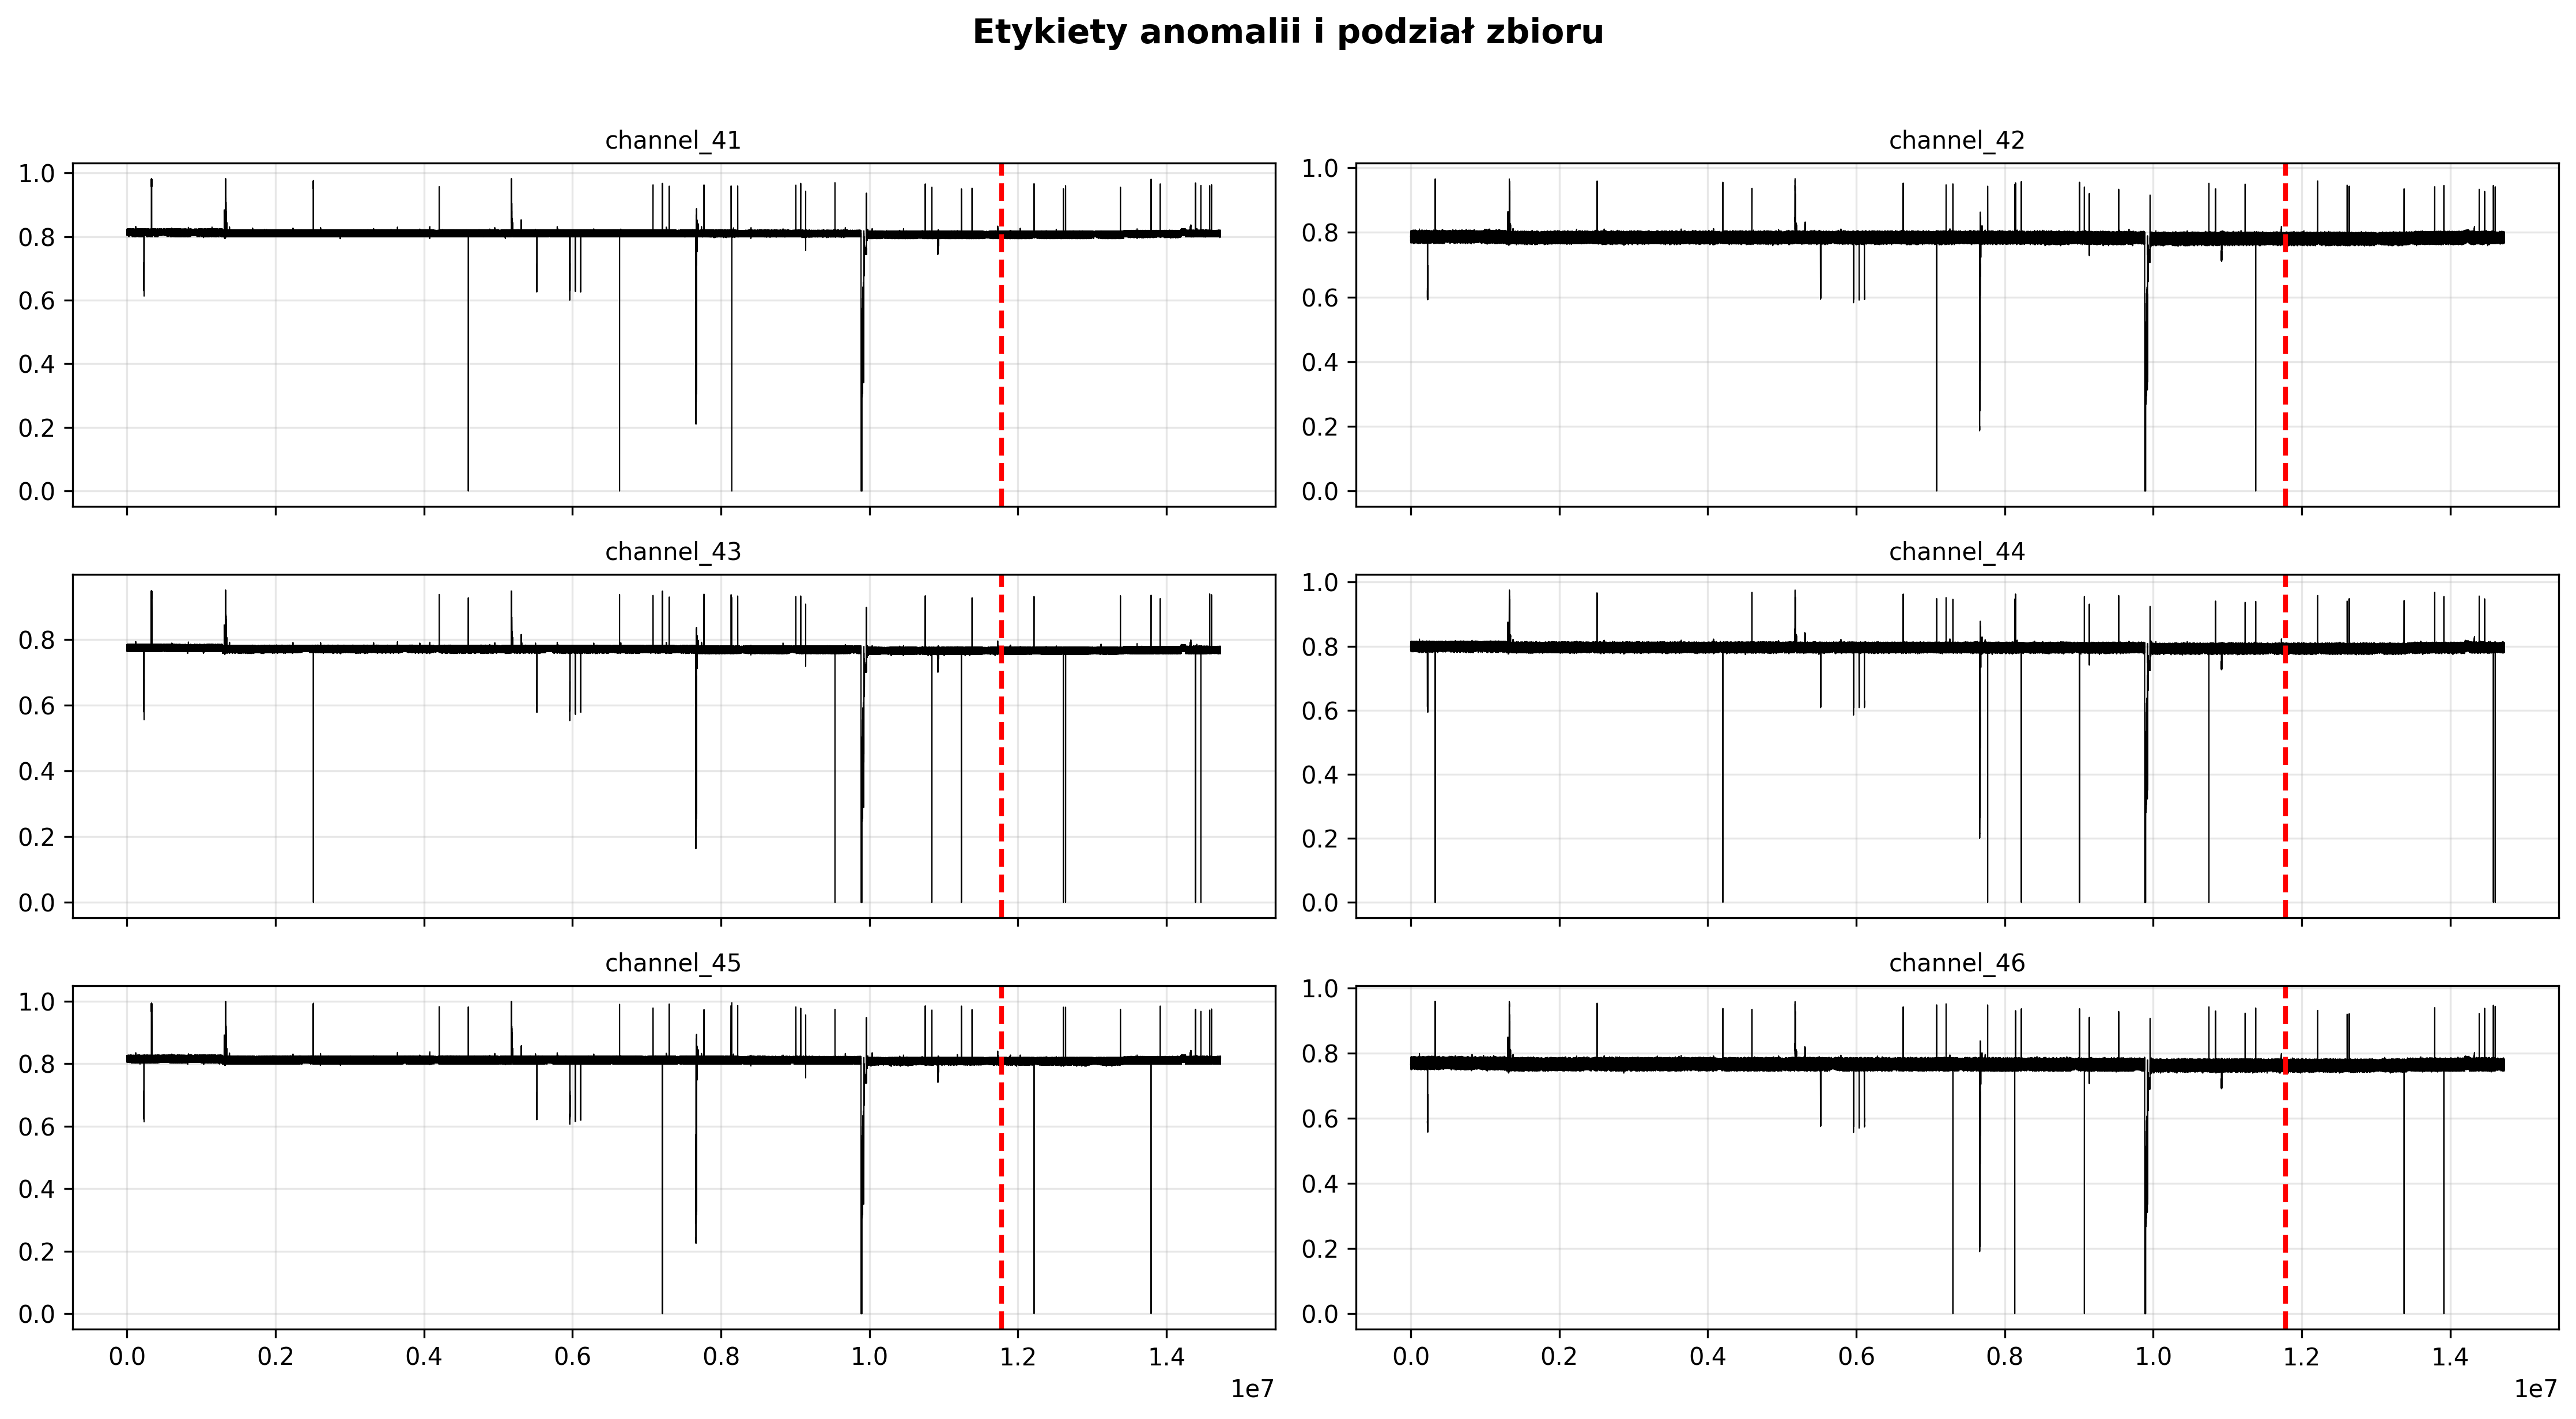
\includegraphics[width=0.9\textwidth]{fig_00_sig_overview.png}
		\caption{Przegląd sygnałów z podziałem chronologicznym 80/20.}
		\label{fig:00-sig-overview}
	\end{figure}
	Rysunek ~\ref{fig:00-sig-overview} przedstawia... umieszczony powyżej przedstawia przegląd rozkładu wartości danych we wszystkich badanych kanałach. Można zauważyć, że czerwona, przerywana linia oznacza linię podziału danych we wszystkich kanałach na zbiory uczące i testując
	\begin{figure}[H]
		\centering
		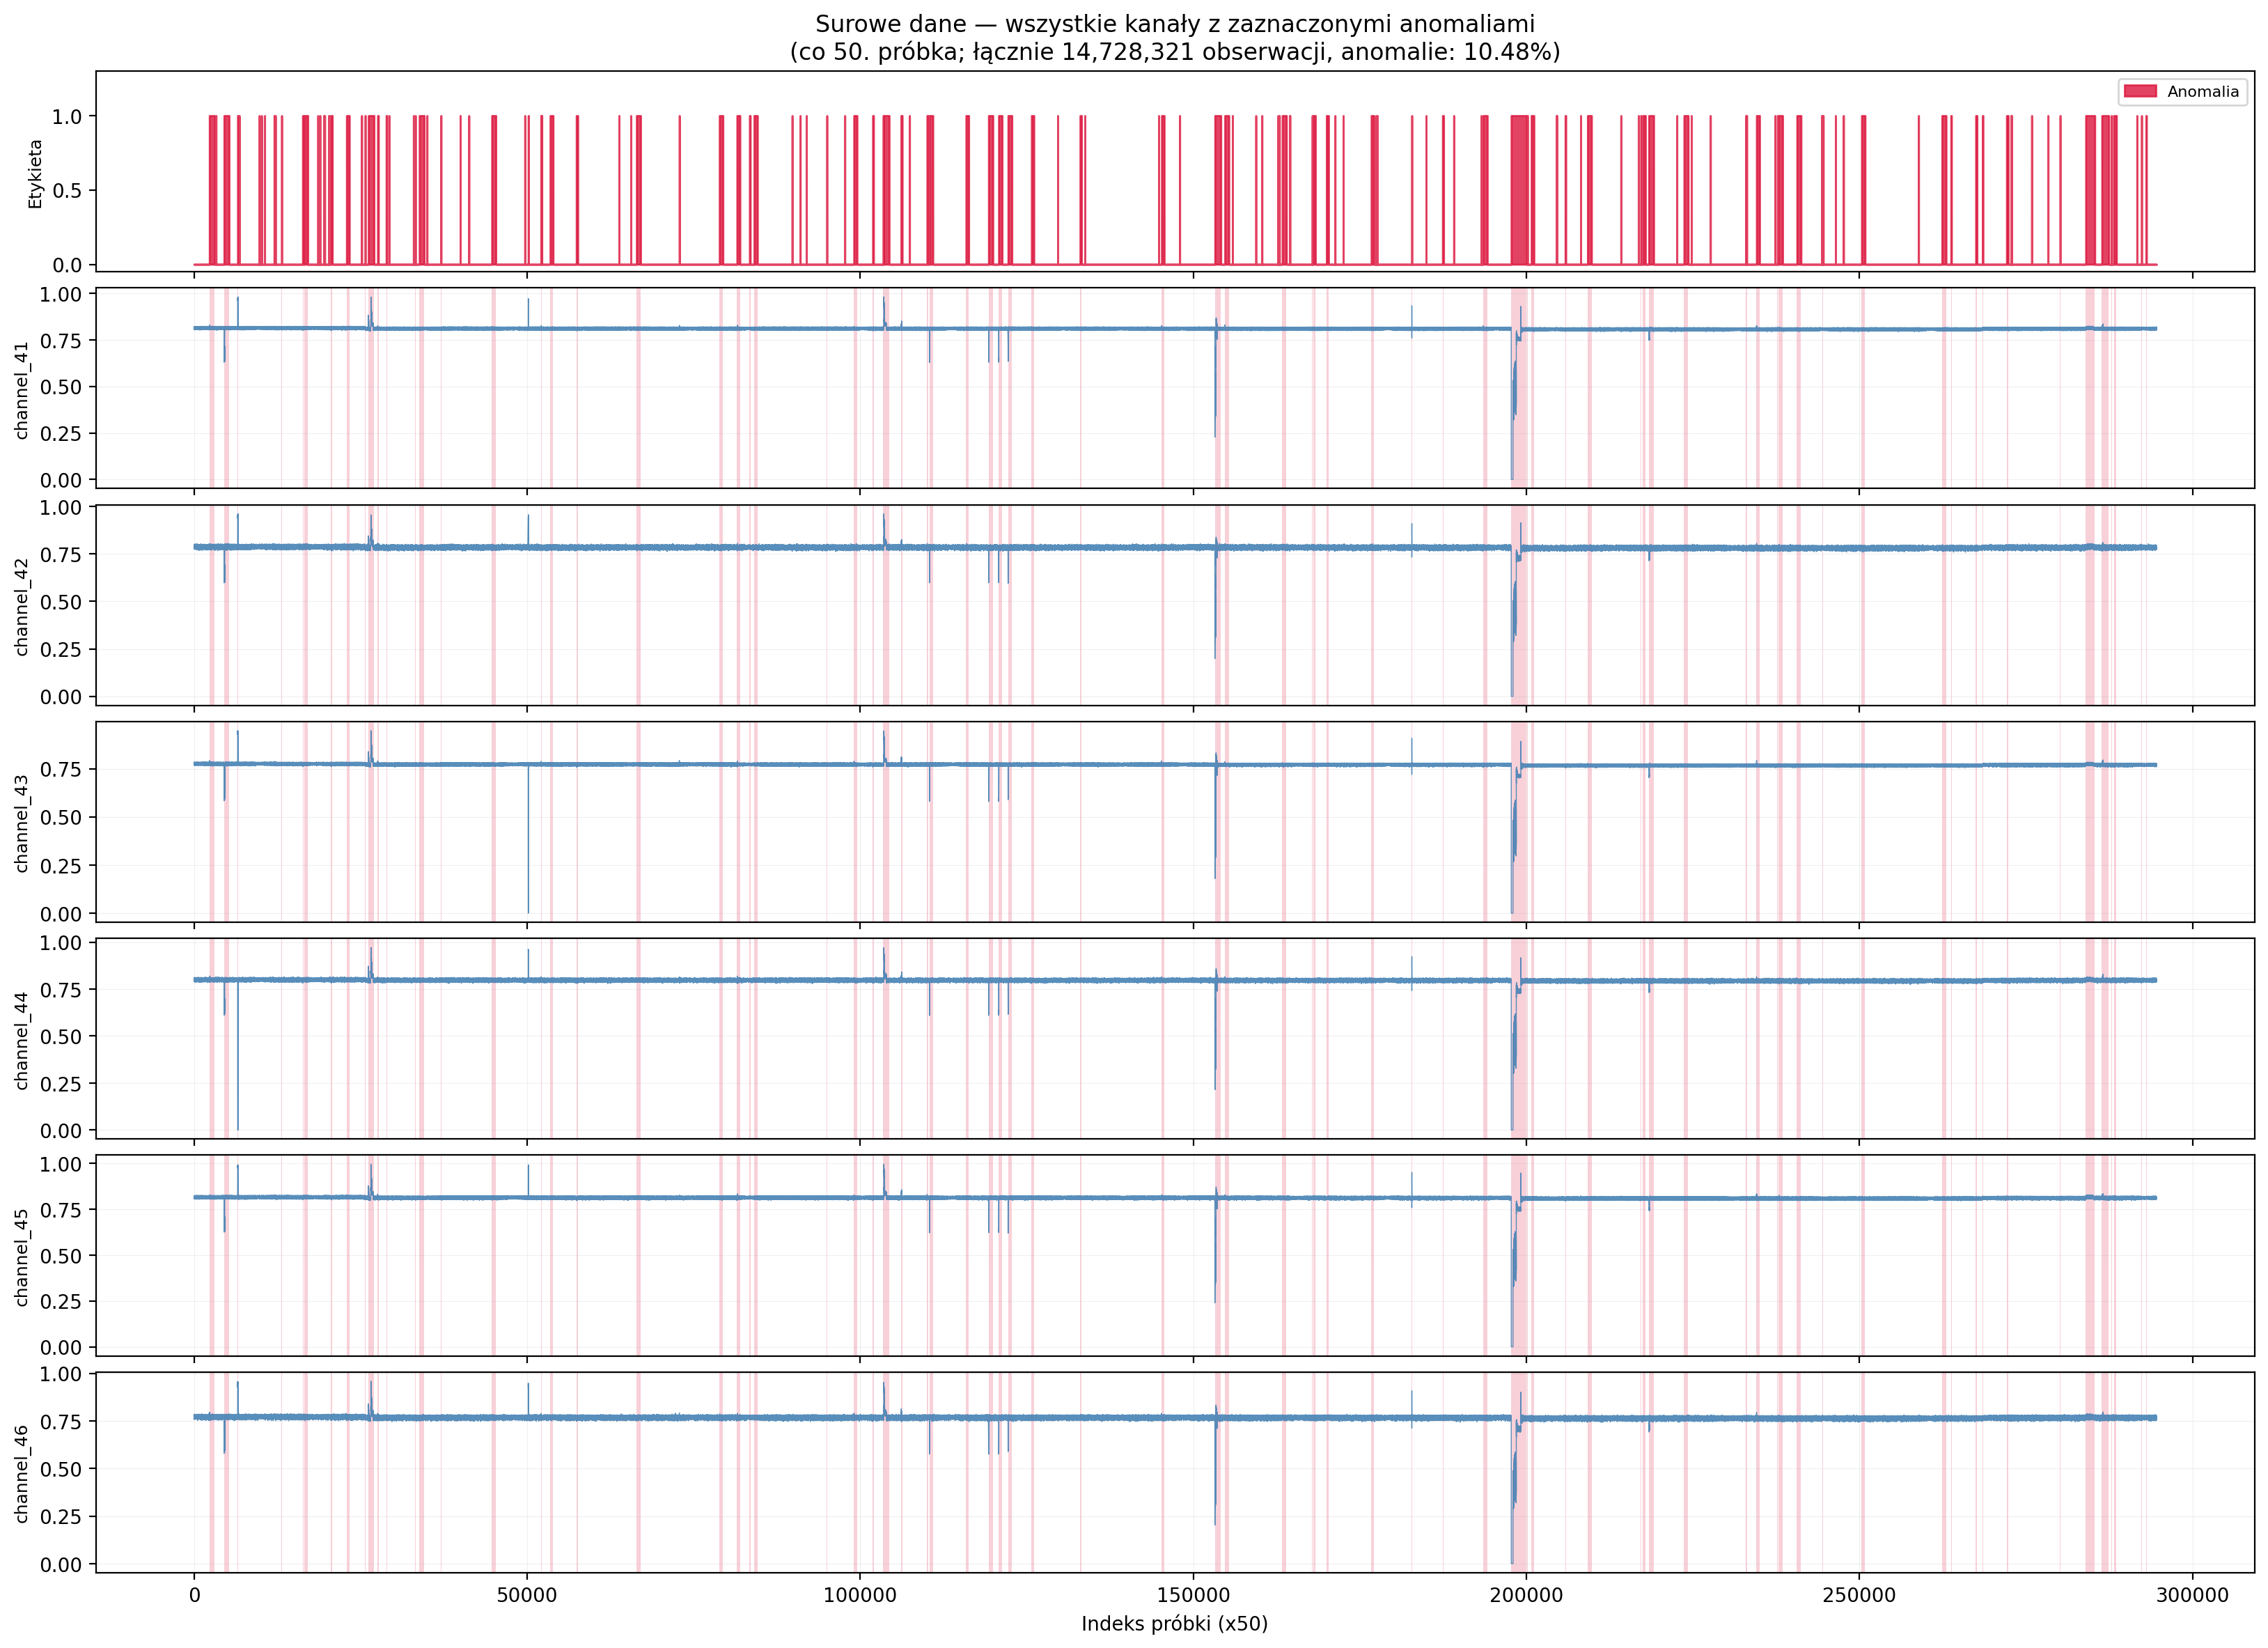
\includegraphics[width=0.9\textwidth]{fig_raw_01_overview.png}
		\caption{Wykres kanałów z występującymi anomaliami}
		\label{fig:raw:01-overview}
	\end{figure}
	
	\begin{figure}[H]
		\centering
		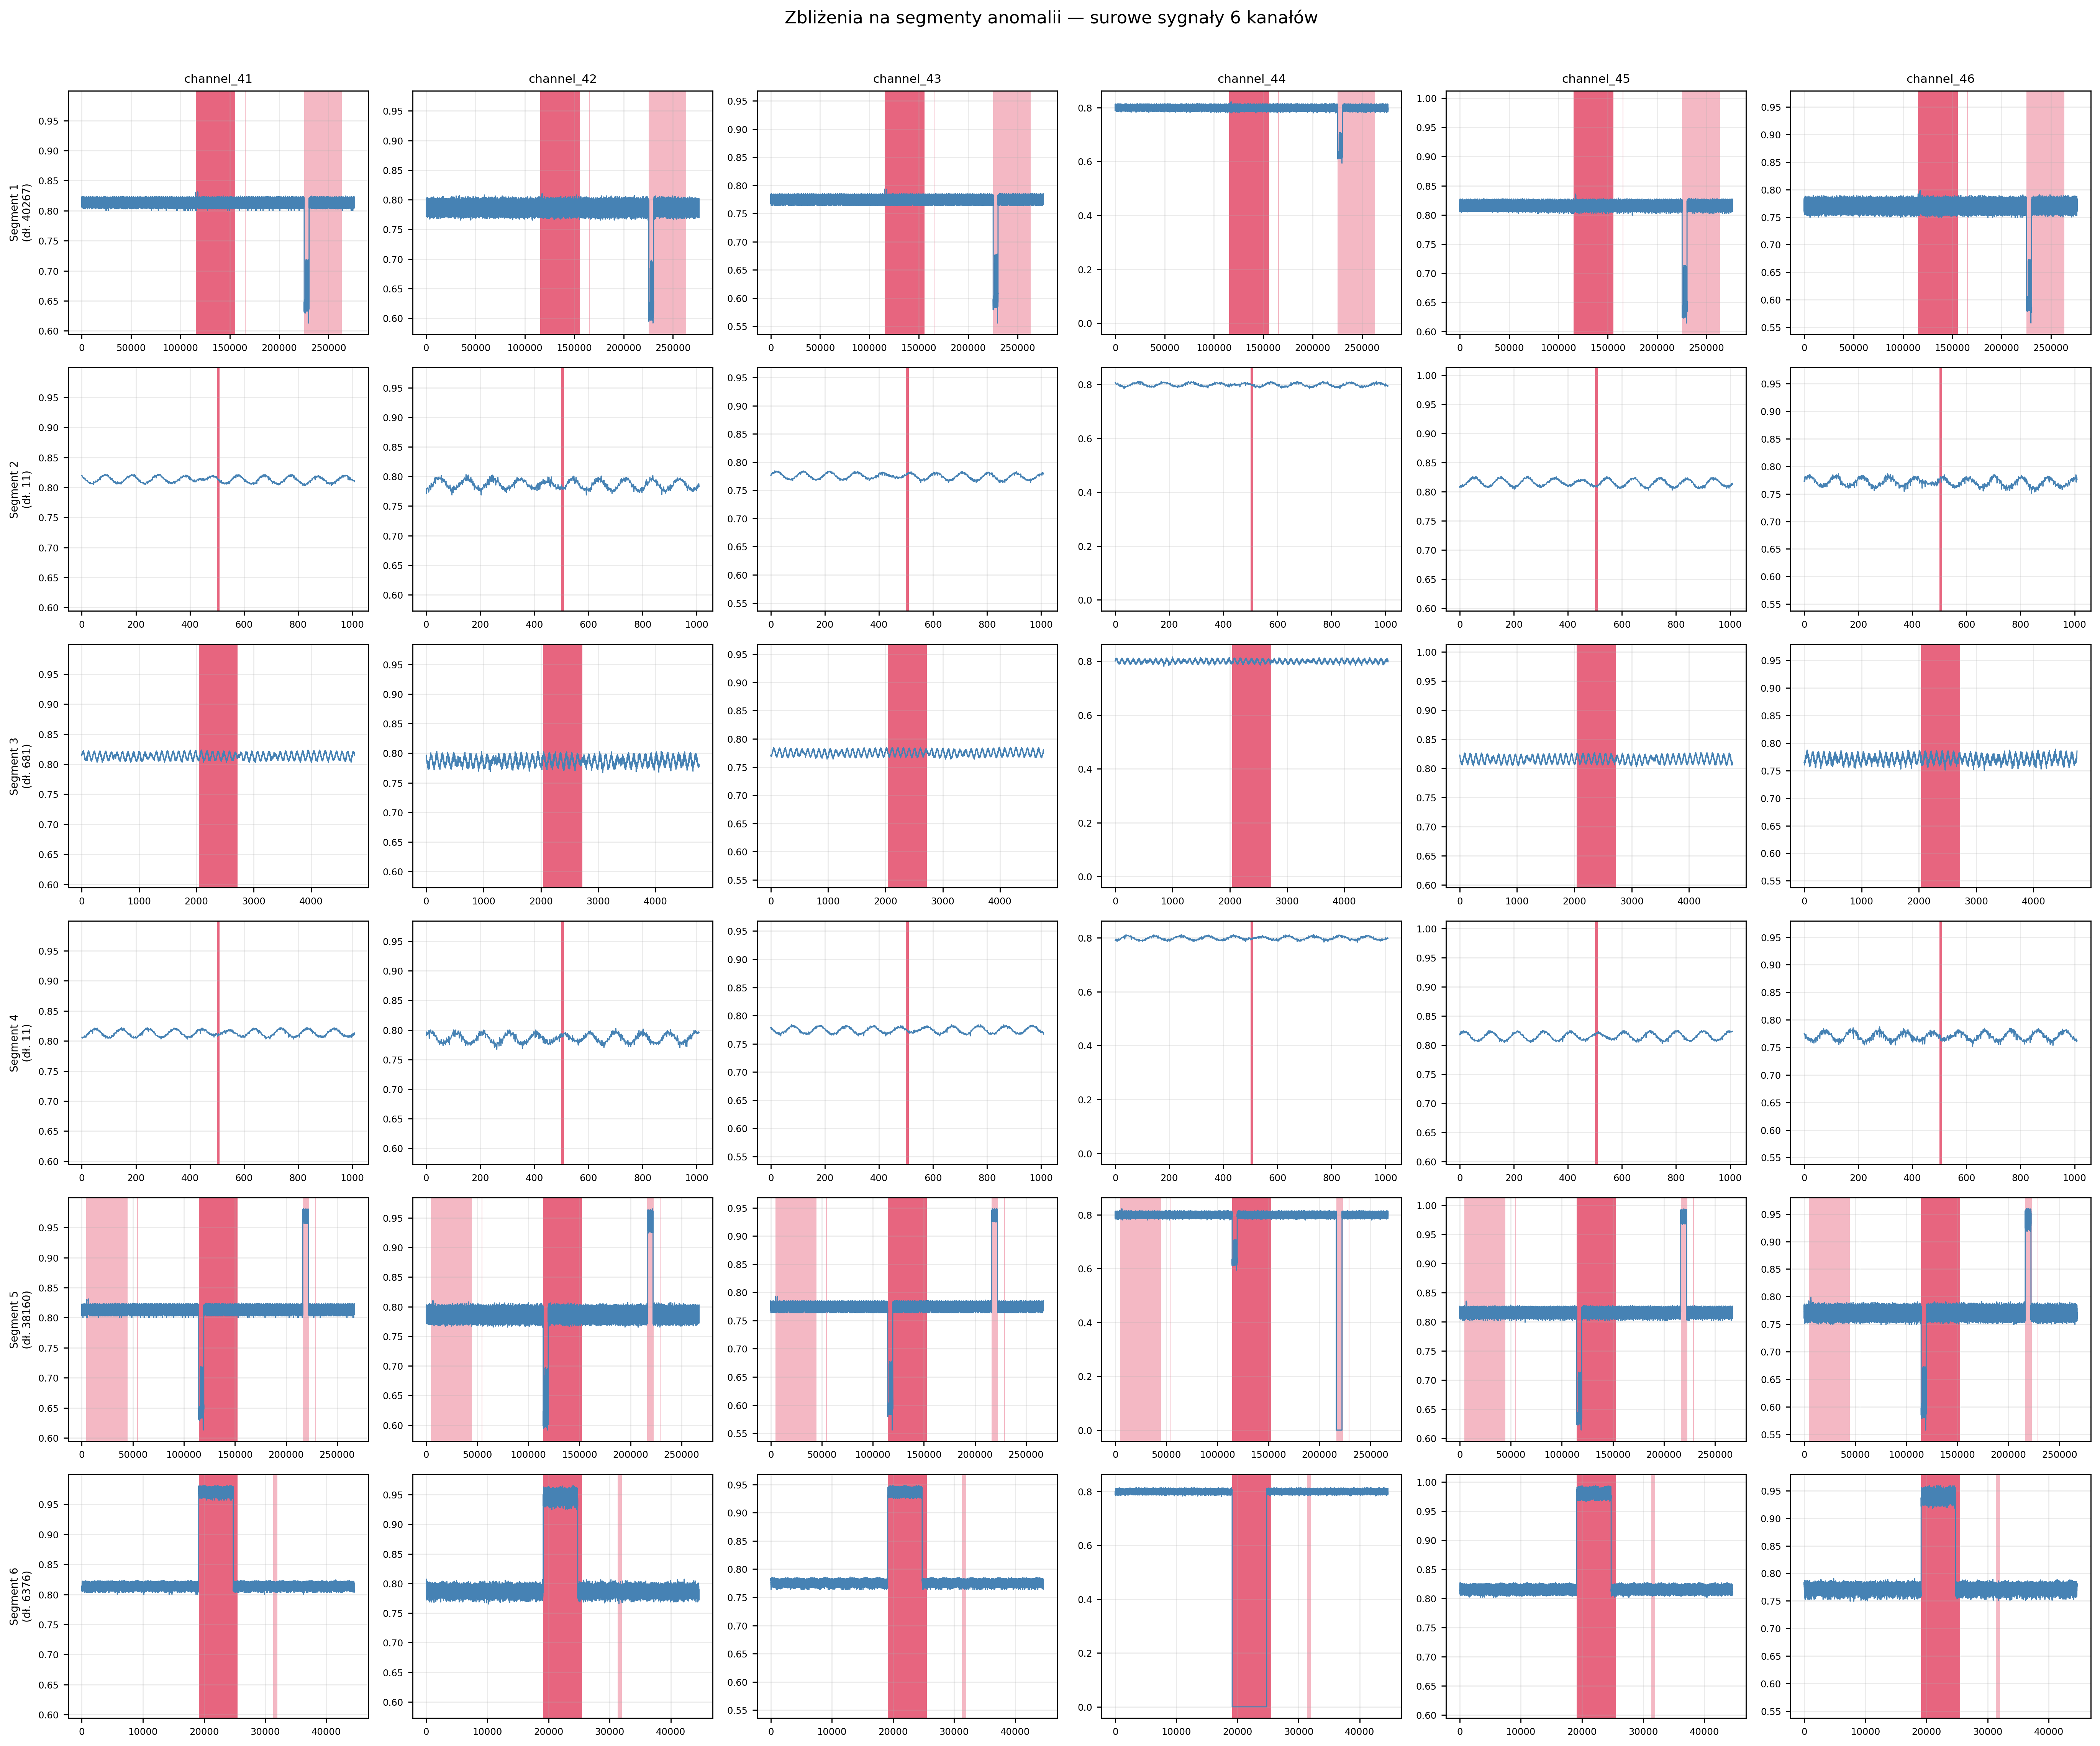
\includegraphics[width=0.9\textwidth]{fig_raw_02_zoom_segments.png}
		\caption{Przybliżone wykresy przedstawiające segmenty z anomaliami}
		\label{fig:raw:02-zoom-segments}
	\end{figure}
	
	Z kolei na rysunku ~\ref{fig:raw:01-overview} ukazano rozkład anomalii w zbiorze, aby pokazać, gdzie się skupiają. W celu ukazania skali pokazano tylko co pięćdziesiątą próbkę, aby pokazać skalę danych na których ewaluowano model. Aby jednak wskazać konkretniej jak wyglądają segmenty anomalii na tle danych normalnych zdecydowano dać przybliżenie na poszczególne segmenty, które zostały ukazane na rysunku ~\ref{fig:raw:02-zoom-segments}. Na obu tych rysunkach anomalie zostały oznaczone na czerwono, a intensywność barwy jest wprost proporcjonalna do gęstości tych danych na obszarze. 
	
	\subsection{Balans klas i rozkład anomalii}
	Na rysunku ~\ref{fig:00-class-balance} umieszczonym poniżej widać jak rozłożenie danych na treningowe i testowe wpływa na odsetek anomalii. W analizowanej próbce, opartej na kanałach od 41 do 46 pierwsza część, czyli 11,7 mln danych zawiera 1,2 mln próbek oznaczonych jako anomalie, co przekłada się na 10,47 procent anomalii. W dalszych częściach badania ta część będzie służyć do uczenia modeli. Pozostała część zbioru, obejmująca pozostałą  część danych, posiada 310 tysięcy anomalii w sobie. Daje to łączenie 10,48 procent anomalii w całości. Oznacza to, że jest to wartość zdecydowanie większa niż w reszcie benchmarku, gdyż średnia danych całości wynosi ledwie 1,8 procent dla danych Mission-1\cite{kotowski2024esaadb}, co czyni badaną część skrajnie niezbilansowaną, co może mieć wpływ na końcowy wynik.
	\begin{figure}[H]
		\centering
		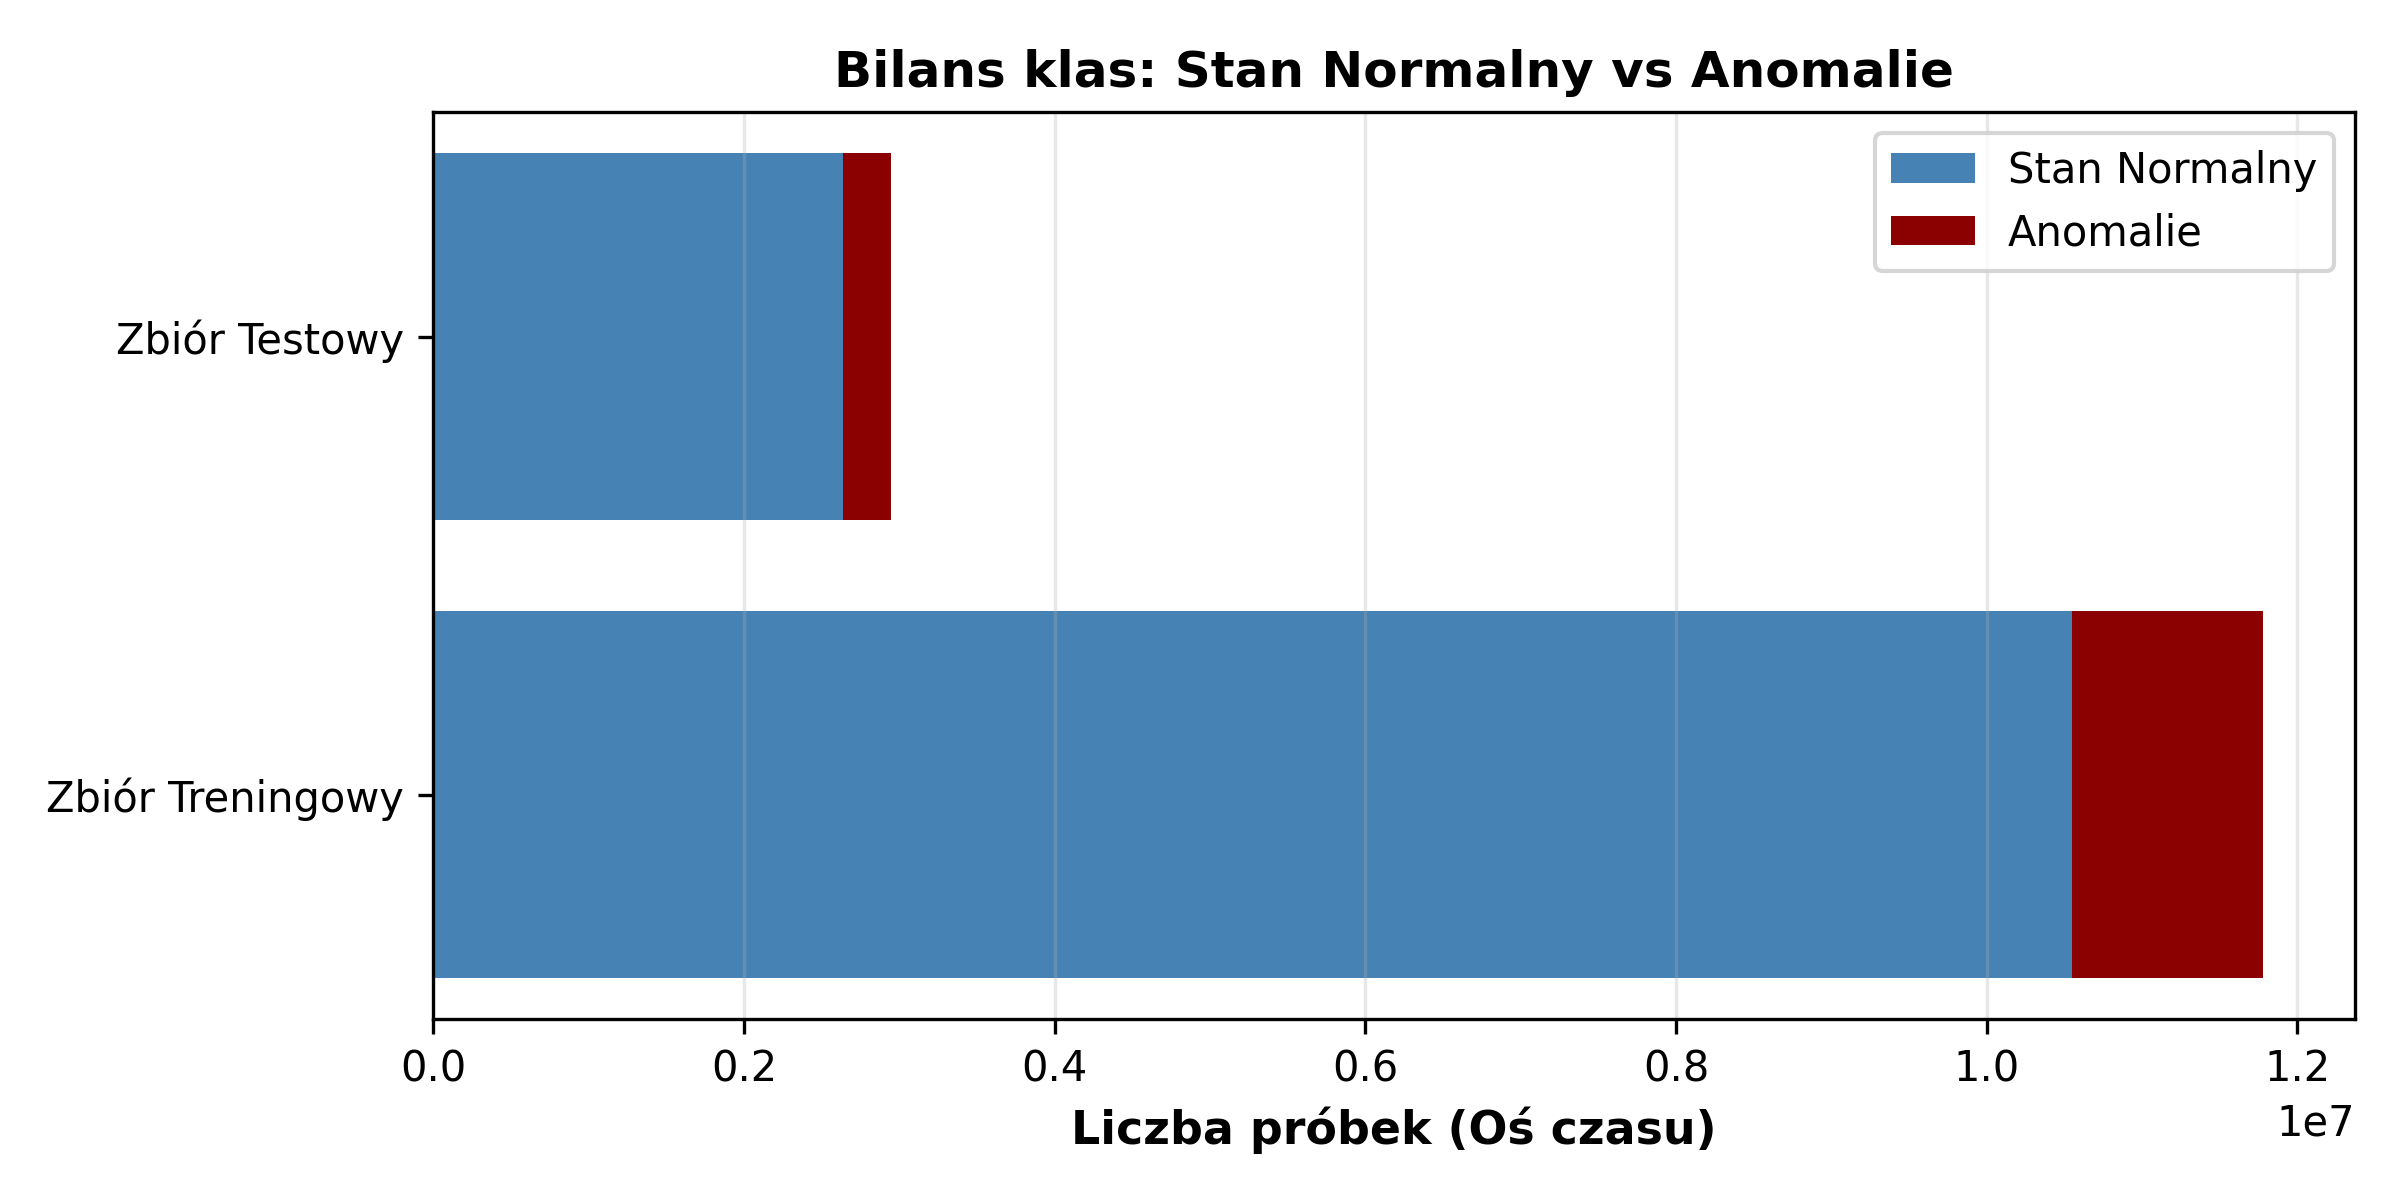
\includegraphics[width=0.9\textwidth]{fig_00_class_balance.png}
		\caption{Bilans klas oraz rozkład występowania anomalii w zbiorach danych.}
		\label{fig:00-class-balance}
	\end{figure}
	Na poniższym rysunku ~\ref{fig:00-anomaly-dist} widać z kolei jak anomalie rozkładają się w poszczególnych zbiorach. Z kolei rysunek ~\ref{fig:raw:03-distributions} przedstawia rozkład wartości surowych dla wszystkich 6 analizowanych kanałów, z wyróżnionym rozróżnieniem na dane normalne i anomalie, w formie histogramu, jakie wartości najczęściej były klasyfikowane. 
	\begin{figure}[H]
		\centering
		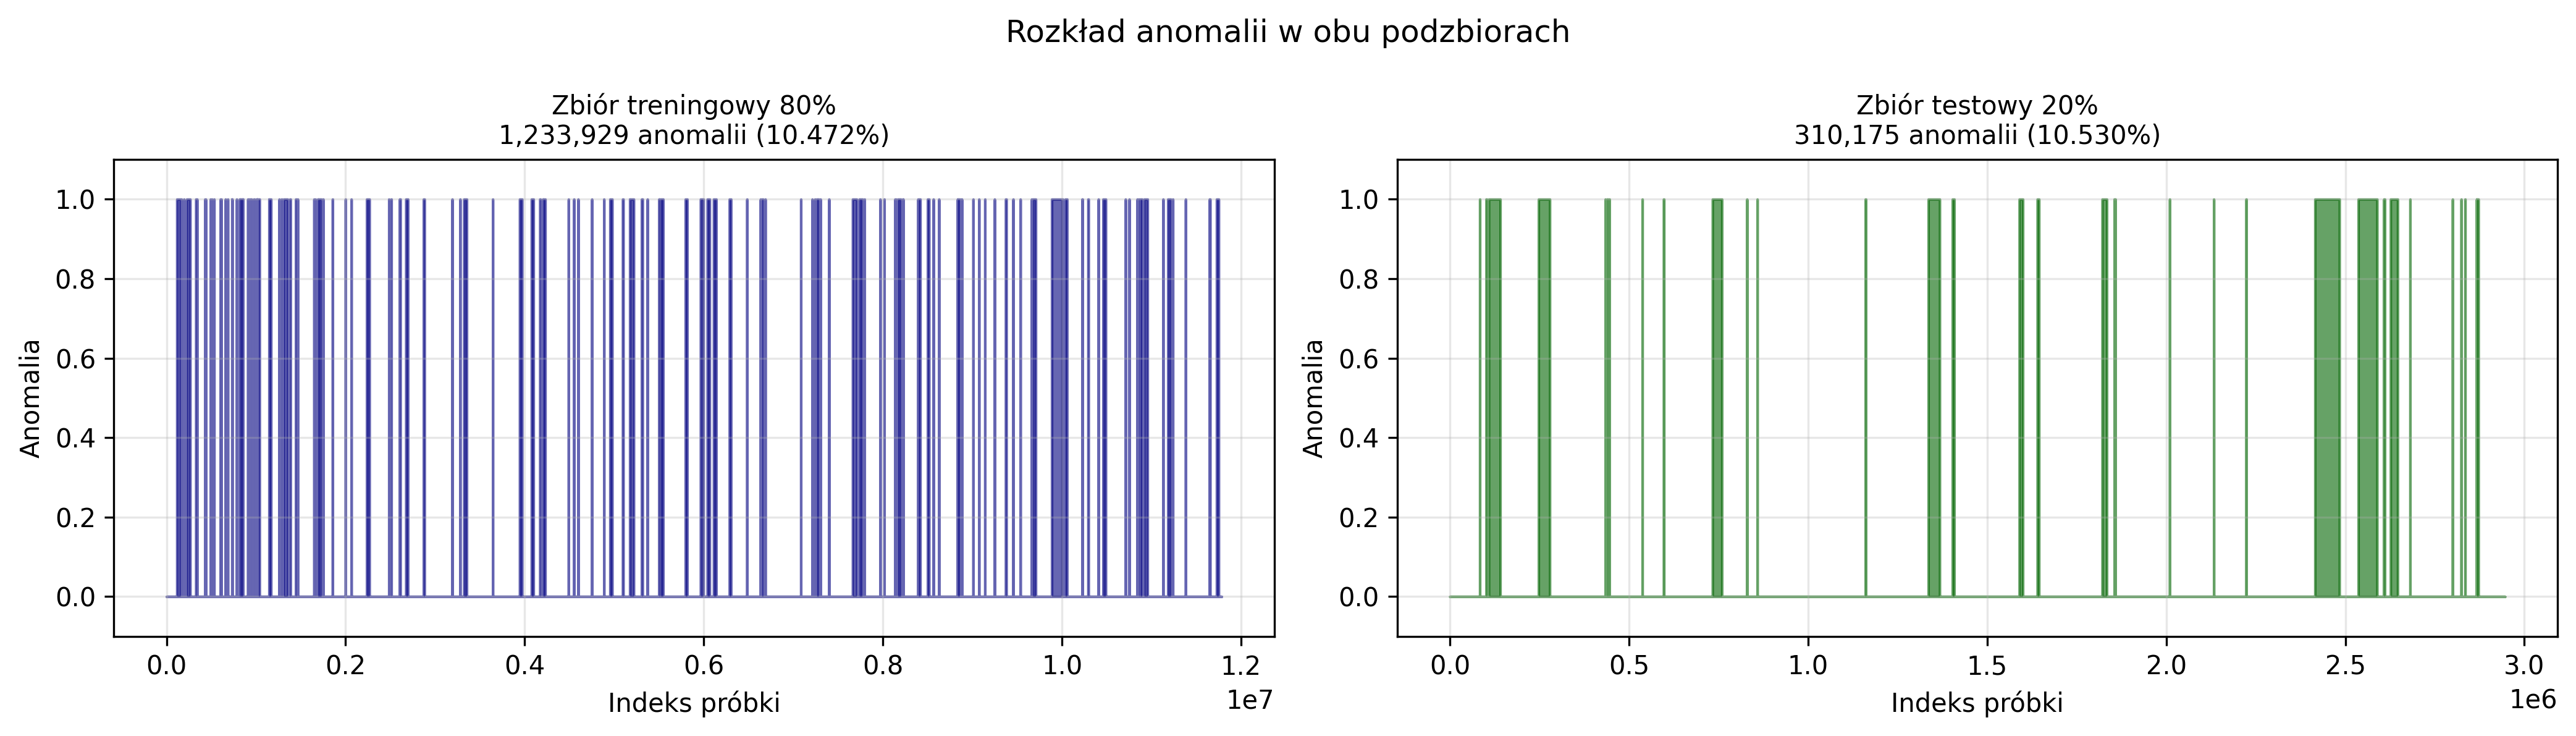
\includegraphics[width=0.9\textwidth]{fig_00_anomaly_dist.png}
		\caption{Rozkład anomalii w zbiorach treningowym i testowym}
		\label{fig:00-anomaly-dist}
	\end{figure}
	
	\begin{figure}[H]
		\centering
		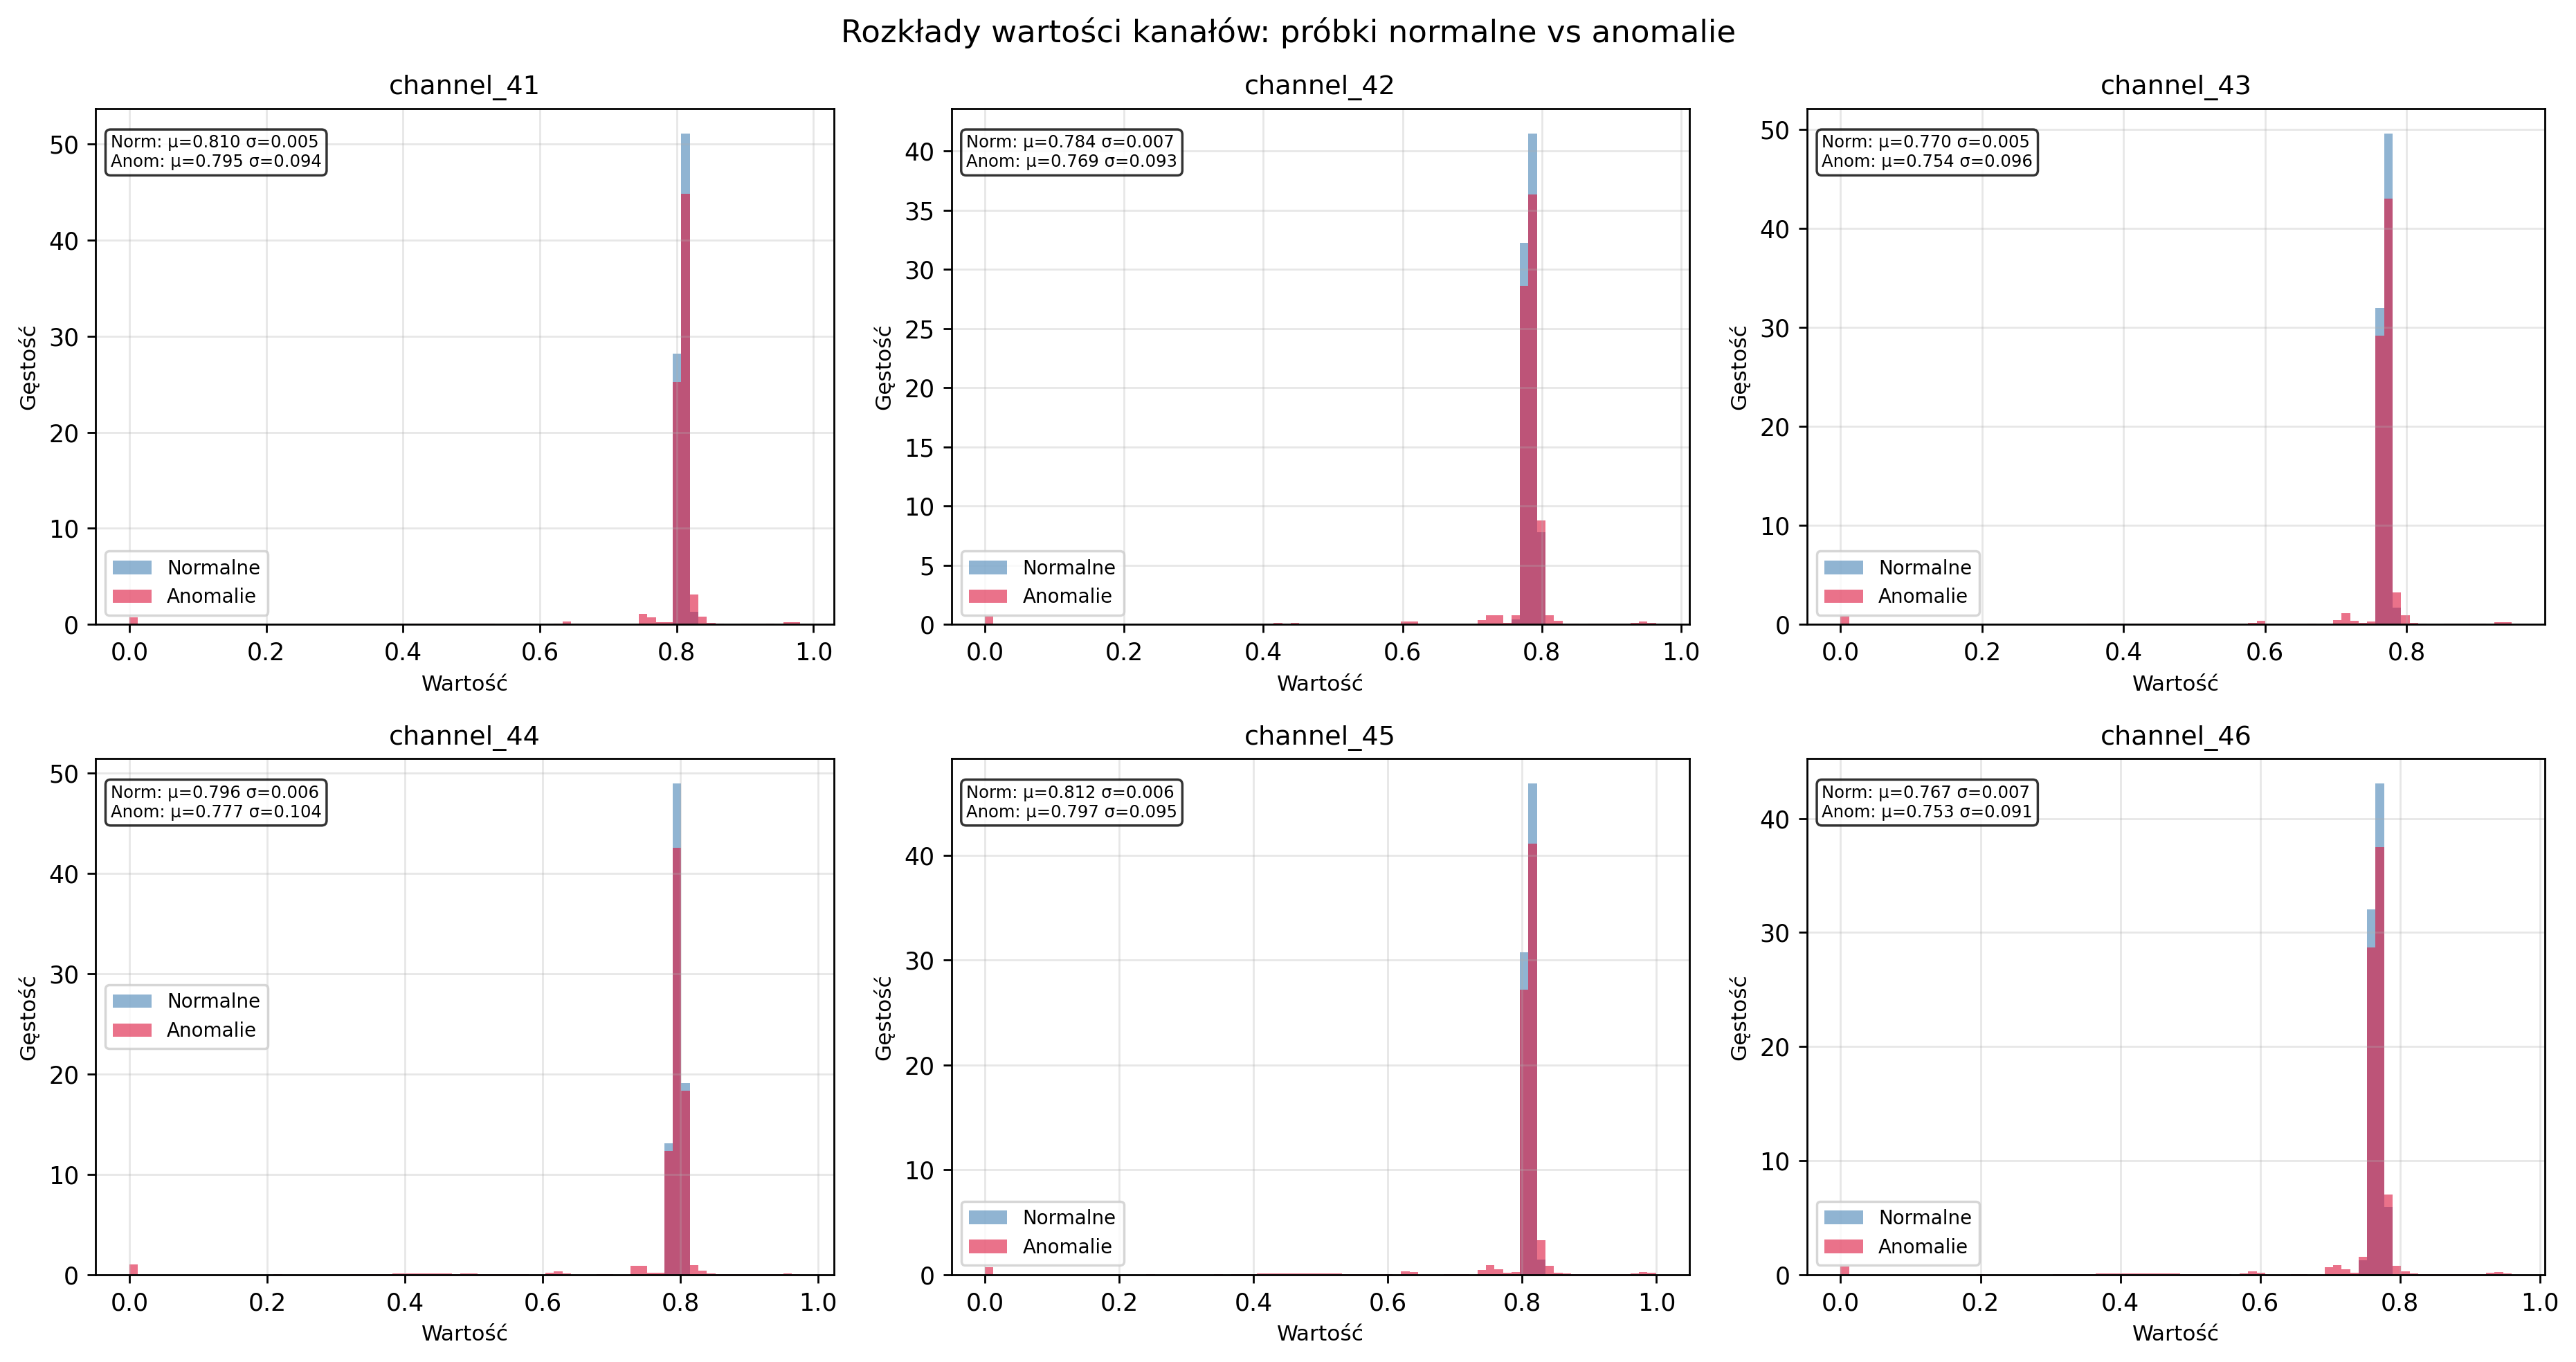
\includegraphics[width=0.9\textwidth]{fig_raw_03_distributions.png}
		\caption{Rozkład wartości kanałów}
		\label{fig:raw:03-distributions}
	\end{figure}
	
	
	
	\section{Środowisko i implementacja}
	Do przeprowadzenia badań wykorzystano laptopa posiadającego procesor AMD Ryzen 5 5600H, posiadający 6 rdzeni i 12 wątków, 16 GB pamięci RAM i zintegrowaną kartę graficzną AMD Radeon™ Graphics z systemem operacyjnym Windows 11. Wszystkie programy zostały wykonane w języku Python w wersji 3.12.2 z wykorzystaniem  poniższych wersji bibliotek:
	\begin{table}[H]
		\centering
		\caption{Wersje najważniejszych bibliotek wykorzystanych w eksperymentach}
		\label{tab:biblioteki}
		\begin{tabular}{ll}
			\hline
			\textbf{Biblioteka} & \textbf{Wersja} \\
			\hline
			Keras & 3.13.0 \\
			Matplotlib & 3.10.8 \\
			NumPy & 1.26.4 \\
			Pandas & 2.3.3 \\
			Scikit-learn & 1.8.0 \\
			TensorFlow & 2.20.0 \\
			TensorFlow Intel & 2.17.0 \\
			TensorFlow IO GCS Filesystem & 0.31.0 \\
			\hline
		\end{tabular}
	\end{table}
	
	Programy zostały wykonane w środowisku Visual Studio Code. W domyślnym folderze ze strukturą projektu znajdują się wszystkie kody spełniające poszczególne funkcje, takie jak przygotowanie danych, inżynieria cech, testowanie wszystkich trzech klas metod i porównanie wszystkich metod pod względem czasu potrzebnego do wykonania poszczególnej iteracji algorytmu z jednym zestawem parametrów, a także zużycia pamięci dla każdej z nich. Każdy program swoje wyniki w osobnym podfolderze folderu „results”. 
	
	
	\section{Preprocessing i inżynieria cech}
	Przed rozpoczęciem właściwych prac dokonano przygotowania danych do właściwego testowania. Dane w momencie publikacji przez Europejską Agencję Kosmiczną już były ustandaryzowane do zbliżonego poziomu do  0-1. Z racji działania na danych chronologicznych, w ramach wzięcia pod uwagę lokalnego kontekstu czasowego, zastosowano technikę okna kroczącego. Polega ona na tym, że dla każdej próbki analizie poddano zarówno bieżącą wartość, jak i ustaloną wartość poprzednich danych. Okno długości w, w chwili t obejmuje próbki od t – w +1 do t.  Używając wartości w tym oknie obliczono trzy cechy opisujące lokalne zachowanie sygnału:
	
	\begin{equation}
		\text{diff}_t = x_t - \mu_t^{(w)}.
	\end{equation}
	
	Pierwszą z nich było odchylenie od lokalnego poziomu bazowego, określa ono jak bardzo wartość bieżąca różniła się od średniego poziomu obserwowanego w szerokości okna kroczącego. Pozwala ono na znalezienie momentu, w którym namierzono sytuację odchylenia sygnału od typowego przebiegu, co może sugerować występowanie anomalii. 
	
	\begin{equation}
		\mu_t^{(w)} = \frac{1}{w} \sum_{i=t-w+1}^{t} x_i,
	\end{equation}
	
	Drugą z nich jest odchylenie standardowe wartości znajdujących się w oknie kroczącym. Im większe okno, tym szerszy zakres. Opisuje lokalną zmianę sygnału. Cecha ta pozwala na znalezienie fragmentu, w którym sygnał stał się nagle niestabilny, lub segmentu z większym rozrzutem danych.
	
	\begin{equation}
		\text{std}_t^{(w)} =
		\sqrt{
			\frac{1}{w}
			\sum_{i=t-w+1}^{t}
			\left(x_i - \mu_t^{(w)}\right)^2
		}.
	\end{equation}
	
	Ostatnią z wartości, którą wyznaczono z pomocą okna kroczącego jest tempo zmiany sygnału pomiędzy próbkami. Pomaga ona namierzyć moment, w którym sygnał gwałtownie zmienia swój charakter. Zależnie od wyniku, może być to skok w górę lub gwałtowny spadek. W ramach badania za tempo zmiany uznano różnicę w charakterze wartości względem pięciu ostatnich próbek.
	
	\begin{equation}
		\text{roc}_t^c = x_t^c - x_{t-5}^c
	\end{equation}
	
	
	
	Wszystkie te cechy mogą tworzyć prostą reprezentację przebiegu sygnału. Po przetworzeniu danych przez okno kroczące każdy z kanałów został opisany dodatkowymi, lokalnymi cechami, a dane wejściowe dla modeli dostały rozszerzoną reprezentację i charakterystykę sygnału. Natomiast to rozwiązanie posiada jeden problem. Dla pierwszych próbek nie można po liczyć cech z pomocą okna kroczącego, bo brakuje wcześniejszych danych tworzących kontekst, który stanowi punkt odniesienia do wyliczania metryk. Proporcjonalnie, im większe okno, tym więcej danych utracono, gdyż wcześniejsze wiersze usunięto. Dzięki temu, każda próbka posiadała pełny zestaw cech. Pomimo tego, że autorzy zbioru dokonali wstępnej normalizacji \cite{kotowski2024esaadb}, obliczone cechy lokalne za pomocą techniki okna kroczącego zostały poddane dodatkowej standaryzacji z-score za pomocą funkcji \textt{StandardScaler}. Parametry zostały wyliczone w ten sposób, czyli odchylenie standardowe i średnia tylko dla danych normalnych zbioru treningowego, co zapobiega przedostaniu się anomalii do modelu.
	
	\section{Dobór okna kroczącego}
	W ramach doboru rozmiaru okna kroczącego przeprowadzono eksperyment testujący wyniki głównych miar w zależności od rozmiaru okna kroczącego, a co za tym idzie cech z nim związanych. Do badań użyto 38 rozmiarów, od pojedynczych jedności, a konkretnie 5, przez dziesiątki, setki, a kończąc na 150 tysiącach jednostek. Natomiast w ramach pierwszej próby użyto tylko okna rozmiarów do ewaluacji od 5 do 5000, aby dać umiarkowane pojęcie o charakterze, wraz z wynikami, w celu znalezienia maksimum, odpowiednio zwiększano granice, aż zwiększanie rozmiarów okien nie dawało poprawy wyników. Do testów użyto algorytmu IQR wraz z wartością mnożnika równą 0.5. Wyniki tego badania pokazuje rysunek ~\ref{fig:01b-large-windows} zamieszczony poniżej.
	\begin{figure}[H]
		\centering
		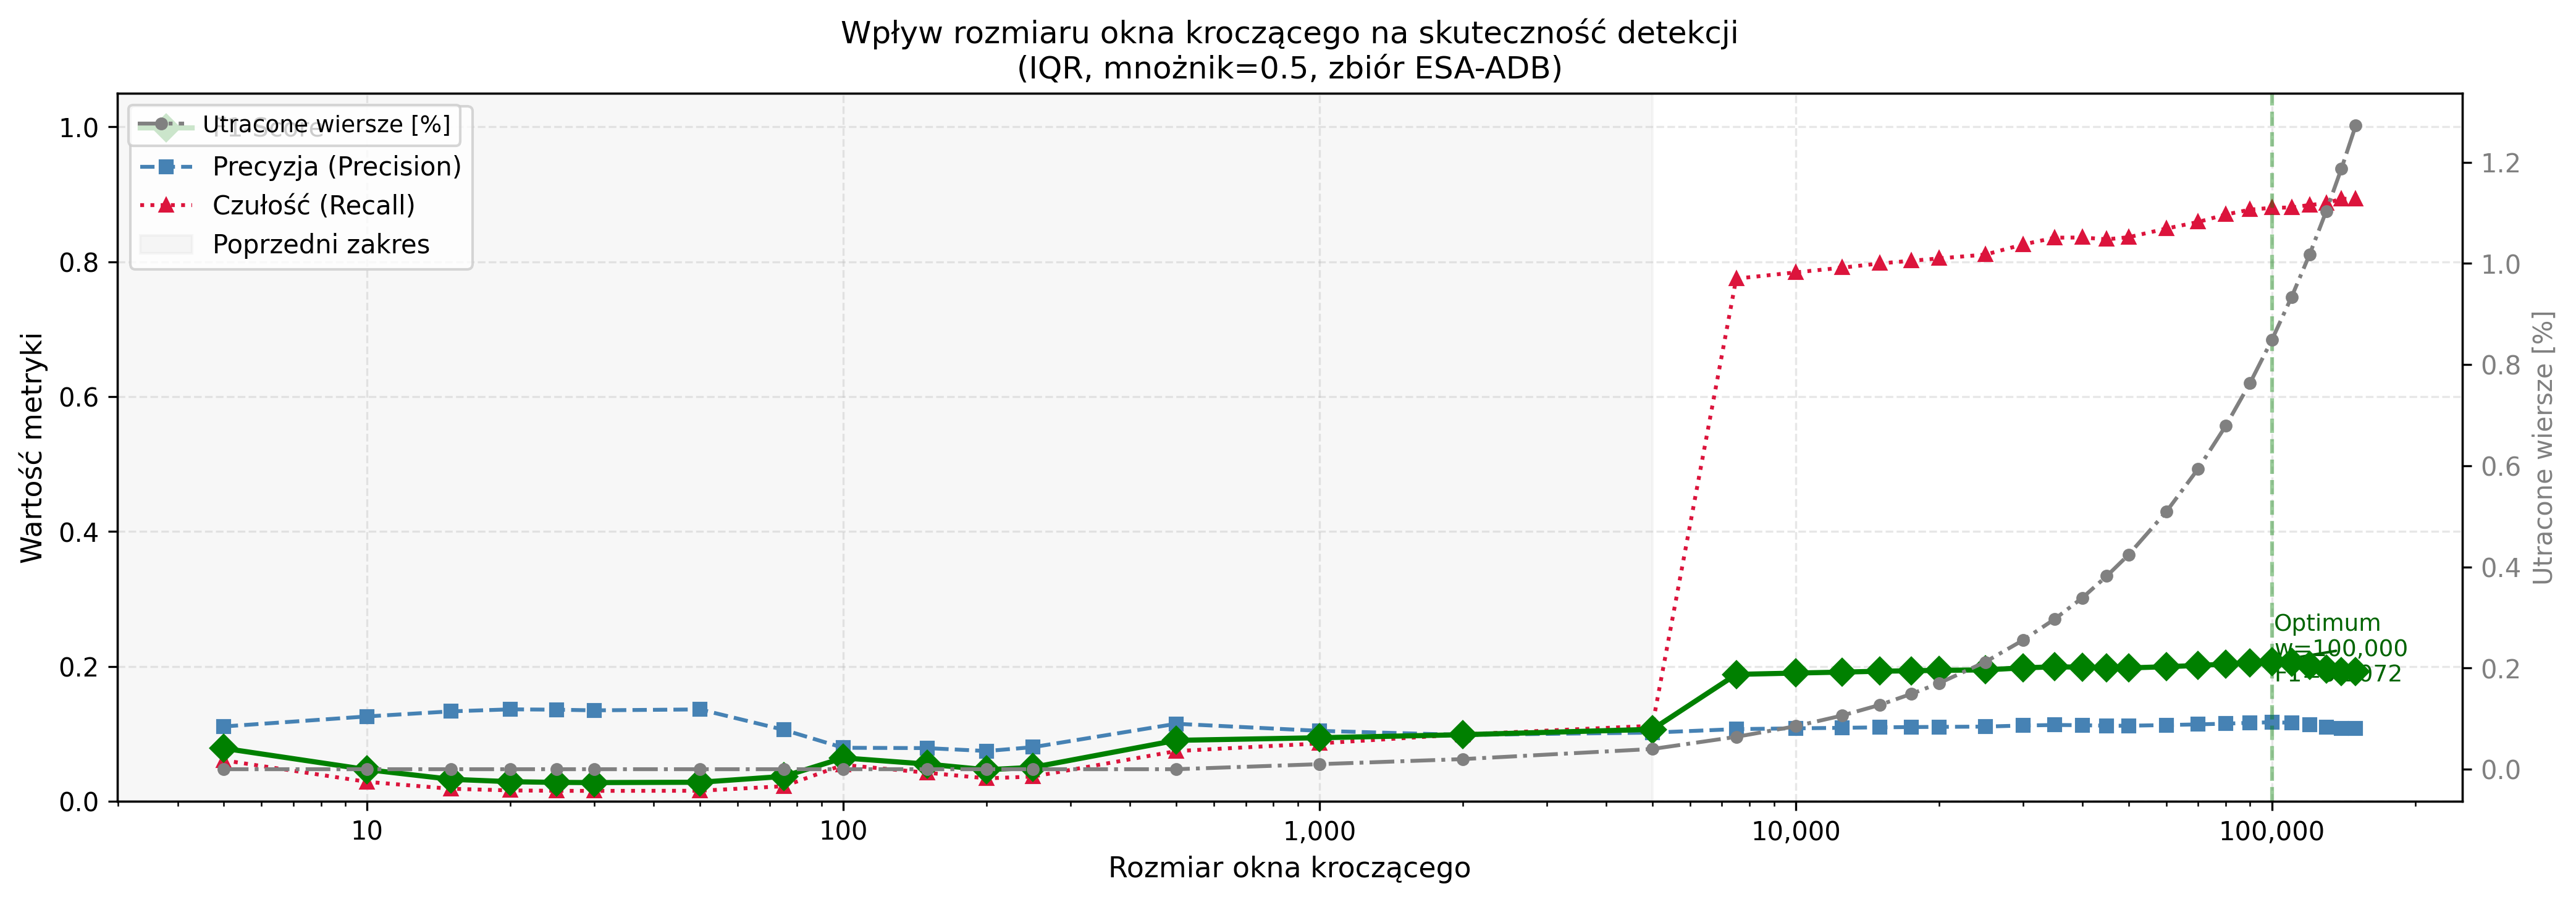
\includegraphics[width=0.9\textwidth]{fig_01b_large_windows.png}
		\caption{Analiza wpływu rozmiaru okna kroczącego na jakość detekcji anomalii.}
		\label{fig:01b-large-windows}
	\end{figure}
	
	
	
	\begin{figure}[H]
		\centering
		
\includegraphics[width=0.9\textwidth]{fig_02b_heatmap.png}
		\caption{Macierz korelacji i wpływu dobieranych parametrów na skuteczność modelu.}
		\label{fig:02-heatmap}
	\end{figure}
	
	Dla początkowych wartości okna wyniki prezentują się mało interesująco, stopniowy wzrost parametru precyzji, do wartości 50, gdzie wartość wyniosła 0.1364, lecz po tym jesteśmy świadkami meandrowania wartości, w jednym momencie rośnie, by wraz z kolejnym, większym rozmiarem powoli spadać. Ogromny skok parametru czułości nastąpił po przejściu z wartości pięciu tysięcy danych na siedem i pół tysiąca. W tym momencie wartość ta z poziomu 0.11 wzrosła aż na 0.775. Czułość, opisana w poprzednim rozdziale, jest to parametr charakteryzujący odsetek poprawnych klasyfikacji spośród wszystkich poprawnie sklasyfikowanych wartości według macierzy pomyłek. Brak skoku w precyzji oznacza natomiast dużą liczbę wartości uznanych za fałszywe pozytywne, dlatego wzrost F1-Score nie okazał się tak okazały, jak w przypadku czułości. Wraz z przekroczeniem progu 1000 danych, zaczęto obserwować także pojawianie się ułamka utraconych danych, z powodu okna kroczącego i jego wymagań. Po zakończeniu eksperymentów uznano, że najlepszą wartością okna okazała się liczba 100000, dla której wartość parametrów F1-Score wyniosła 0.2072, precyzja wyniosła 0.1174, a czułość 0.8801, przy około 0.849 procenta danych utraconych. Pełen rozkład wartości głównych miar prezentuje rysunek ~\ref{fig:02-heatmap} umieszczony powyżej. W dalszych badaniach ewaluujących metody statystyczne, uczenia maszynowego i głębokiego uczenia użyto tego rozmiaru do wyliczenia lokalnych cech pomagających algorytmom w trakcie wykonywanego zadania.
	
	\section{Punkt odniesienia}
	
	Rygorystyczna idea badawcza we współczesnych czasach, w epoce dostępności algorytmów uczenia maszynowego i głębokiego, jednym ze sposobów przygotowania do zaawansowanej analizy algorytmów jest wprowadzenia wyniku pewnej wartości algorytmu jako punkt odniesienia, zwanego z ang. \english{baseline}. Punktem tym jest punkt przyjmowany jako minimalny próg skuteczności ewaluacji. Z powodu znacznego złożenia algorytmów uczenia maszynowego i głębokiego (znanych pod skrótami ML i DL) i kosztów obliczeniowych jakie generują w trakcie wykonywania algorytmu, lub uczenia sieci, czasowych i infrastruktury, ich zastosowanie musi być uwarunkowane istotną poprawą wyników w porównaniu do prostych, mało złożonych, można powiedzieć trywialnych, metod statystycznych. 
	W niniejszej pracy postanowiono przyjąć zoptymalizowaną metodę IQR, po serii badań doboru mnożnika różnicy i wpływu na wyniki. Punkt odniesienia osiągnięty przez ten algorytm na zbiorze testowym posiada następujące miary: F1=0.2211, precyzja wynosi 0.1304, a czułość była równa 0.7279.
	Charakterystyka wyników ukazana w tym eksperymencie przed właściwą częścią badań, głównie niska precyzja, przy względnie dużej czułości, jest dość powszechna dla prostych metod polegających na analizowaniu pojedynczego punktu. Metoda IQR sprawdziła się poprawnie wychwytując większość odchyleń w sygnale, co ukazuje miara czułości. Lecz nawet po implementacji okna kroczącego, dającego lokalny kontekst, metoda jest ograniczona pod względem analizy wielowymiarowej danych. W złożonych systemach mierzących anomalie nie są tylko ekstremum na pojedynczym kanele, a raczej nietypową korelacją między kilkoma czujnikami ( np. spadek ciśnienia z nagłym wzrostem temperatury w hipotetycznym scenariuszu). Metoda IQR ma problem z odróżnieniem prawdziwej awarii od względnie nieszkodliwego szumu na kilku kanałach, co może powodować ogromną liczbę fałszywych alarmów obniżających precyzję. Dlatego owa metoda jest dobrą propozycją punktu wyjścia do dalszej weryfikacji, jak bardzo inne metody statystyczne, nieliniowe modele uczenia maszynowego i głębokiego, mogą poprawić wyniki tego punktu odniesienia 
	
	
	\section{Metodologia badań}
	W celu zapewnienia rzetelności, powtarzalności i jakości przeprowadzonych badań, wszystkie testowane algorytmy zostały poddane eksperymentom. Z powodu pracy nad ciągłymi szeregami czasowymi z dużą ilością próbek badawczych, biorąc pod uwagę fakt, że badany zbiór jest małym odłamkiem pełni zbioru udostępnionego przez Europejską Agencję Kosmiczną, trzeba było wprowadzić pewne kompromisy. 
	
	Przetwarzanie pełnego zbioru danych ESA-ADB, który posiada blisko 15 milionów próbek, stanowi ogromne, w pewnych przypadkach niewykonalne, wyzwanie dla używanej platformy sprzętowej. O ile metody statystyczne (np. Z-Score, czy EWMA) są proste pod kątem złożoności liniowej i nie posiadały większych problemów w testowaniu całości zbioru w miarę rozsądnym czasie, o tyle klasyczne algorytmy uczenia maszynowego, jak np. Local Outlier Factor, czy One-Class SVM charakteryzują się zdecydowanie większym poziomem złożoności. Wytrenowanie algorytmów na pełnym zbiorze prowadziła do błędów związanych z przepełnieniem pamięci operacyjnej. Dlatego, z tego powodu, dla metod uczenia maszynowego i sieci rekurencyjnych, jak autoenkoder oparty o LSTM, których algorytm wykorzystuje ogromne ilości zasobów, konieczne było ograniczenie próbki badawczej, na których metody mają wykrywać anomalie. Zmniejszenie próbki badawczej pozwoliło na bezpieczne dla platformy przeprowadzenie badań w miarę rozsądnym oknie czasowym, przy jednoczesnym zachowaniu charakterystyki rozkładu cech fizycznych sygnału. Natomiast koniecznym do wyróżnienia faktem jest zachowanie nienaruszonego zbioru testowego. 
	
	Optymalizowanie parametrów poszczególnych metod przeprowadzono z użyciem metody przeszukiwania siatki (ang. \english{Grid Search}). Świadomie zrezygnowano z walidacji krzyżowej. Podjęto tą decyzję, pod wpływem ogromnej objętości danych i złożoności obliczeniowej, pojedynczy cykl uczenia modeli uczenia maszynowego, a zwłaszcza sieci neuronowych do metod DL trwało godzinami, co czyniło wielokrotne trenowanie trudnymi do wykonania w rozsądnym czasie. Warto zaznaczyć, że w  przypadku szeregów czasowych o rozmiarach rzędu milionów próbek, podział chronologiczny, zapewnia wystarczającą stabilność wyników i zmniejsza ryzyko przypadkowości do minimum, co czynu walidację krzyżową zbędną.
	
	W metodach bazujących na kompresji i rekompresji sygnału (autoenkoderach) z użyciem sieci gęstych, głębokich i rekurencyjnych, jednym z głównych wyzwań jest przekształcanie błędu rekonstrukcji w zero-jedynkową decyzję o tym czy jest to anomalia, czy nie. W celu jednolicenia metodologii badań przyjęto metodykę opartą na rozkładzie błędów zbioru treningowego. Model wnioskował na bazie danych uczących, które były podstawą do obliczenia błędów rekonstrukcji sygnału. Następnie za statyczny próg odcięcia (ang. \english{threshold}) wyznaczono 90 percentyl tego rozkładu błędów. Uznano, że 10 procent marginesu tolerancji to naturalny szum maszyny. W związku z tym, każdy błąd rekonstrukcji, który przewyższy ten próg, został uznany za anomalię.
	
	Po uzyskaniu wyników uznano, że wszystkim miarom uzyskanym w trakcie badania potrzeba nadać rygor i wyeliminować wpływ losowości i przypadku. W ramach tego procedurę badawczą rozszerzono o testy statyczne. Zastosowano kombinację podejść:
	\begin{itemize}
		\item \textbf{Przedziały ufności (Bootstrap Confidence Intervals):}. Skuteczność miary F1-Score na zbiorze testowym została zweryfikowana z pomocą losowania ze zwracaniem, co pozwoliło na oszacowanie wariancji danego modelu i wyznaczenia przedziałów ufności dla uzyskanych miar, co wzmacnia stabilność poszczególnych algorytmów.
		\item \textbf{Test McNemara:}Test McNemara Aby porównać modele między sobą w parach wykorzystano test McNemara, czyli test nieparametryczny analizujący macierz błędów krzyżowych, co jest adekwatnym rozwiązaniem do weryfikacji wyników na sparowanym zbiorze testowym. Pozwala to na dowód matematyczny istotności statystycznej przewagi metod uczenia głębokiego, wykluczając przypadek na poziomie $\alpha = 0.05$.
	\end{itemize}
	
	%\begin{figure}
	%\centering
	%\begin{tikzpicture}
	%\begin{axis}[
	%    y tick label style={
		%        /pgf/number format/.cd,
		%            fixed,   % po zakomentowaniu os rzednych jest indeksowana wykladniczo
		%            fixed zerofill, % 1.0 zamiast 1
		%           precision=1,
		%        /tikz/.cd
		%    },
	%    x tick label style={
		%       /pgf/number format/.cd,
		%%         fixed zerofill,
		%        precision=2,
		%    /tikz/.cd
		%}
	%]
	%\addplot [domain=0.0:0.1] {rnd};
	%\end{axis} 
	%\end{tikzpicture}
	%\caption{Wykres przebiegu funkcji.} % Podpis jest zawsze POD rysunkiem.
	%\label{fig:2}
	%\end{figure}
	
	
	%%%%%%%%%%%%%%%%%%%%%
	%% RYSUNEK Z PLIKU
	%
	%\begin{figure}
	%\centering
	%
\includegraphics[width=0.5\textwidth]{./politechnika_sl_logo_bw_pion_pl.pdf}
	%\caption{Podpis rysunku zawsze pod rysunkiem.}
	%\label{fig:etykieta-rysunku}
	%\end{figure}
	%Rys. \ref{fig:etykieta-rysunku} przestawia …
	%%%%%%%%%%%%%%%%%%%%%
	%
	%%%%%%%%%%%%%%%%%%%%%
	%% WIELE RYSUNKÓW 
	%
	%\begin{figure}
	%\centering
	%\begin{subfigure}{0.4\textwidth}
	%    
\includegraphics[width=\textwidth]{./politechnika_sl_logo_bw_pion_pl.pdf}
	%    \caption{Lewy górny rysunek.}
	%    \label{fig:lewy-gorny}
	%\end{subfigure}
	%\hfill
	%\begin{subfigure}{0.4\textwidth}
	%    
\includegraphics[width=\textwidth]{./politechnika_sl_logo_bw_pion_pl.pdf}
	%    \caption{Prawy górny rysunek.}
	%    \label{fig:prawy-gorny}
	%\end{subfigure}
	%
	%\begin{subfigure}{0.4\textwidth}
	%    
\includegraphics[width=\textwidth]{./politechnika_sl_logo_bw_pion_pl.pdf}
	%    \caption{Lewy dolny rysunek.}
	%    \label{fig:lewy-dolny}
	%\end{subfigure}
	%\hfill
	%\begin{subfigure}{0.4\textwidth}
	%    
\includegraphics[width=\textwidth]{./politechnika_sl_logo_bw_pion_pl.pdf}
	%    \caption{Prawy dolny rysunek.}
	%    \label{fig:prawy-dolny}
	%\end{subfigure}
	%        
	%\caption{Wspólny podpis kilku rysunków.}
	%\label{fig:wiele-rysunkow}
	%\end{figure}
	%Rys. \ref{fig:wiele-rysunkow} przestawia wiele ważnych informacji, np. rys. \ref{fig:prawy-gorny} jest na prawo u góry.
	%%%%%%%%%%%%%%%%%%%%%
	
	
	%\chapter{[Przedmiot pracy]}
	%
	%\begin{itemize}
	%\item  Jak ja rozwiązuję problem?
	%\begin{itemize}
	%\item rozwiązanie zaproponowane przez dyplomanta
	%\item analiza teoretyczna rozwiązania
	%\item uzasadnienie wyboru zastosowanych metod, algorytmów, narzędzi
	%\end{itemize}
	%\end{itemize}
	
	
	% TODO
	\chapter{Eksperymenty i wyniki}
	
	\section{Metoda IQR - pierwszy próg}
	
	
	
	
	\section{Wyniki metod statystycznych}
	
	\begin{figure}[H]
		\centering
		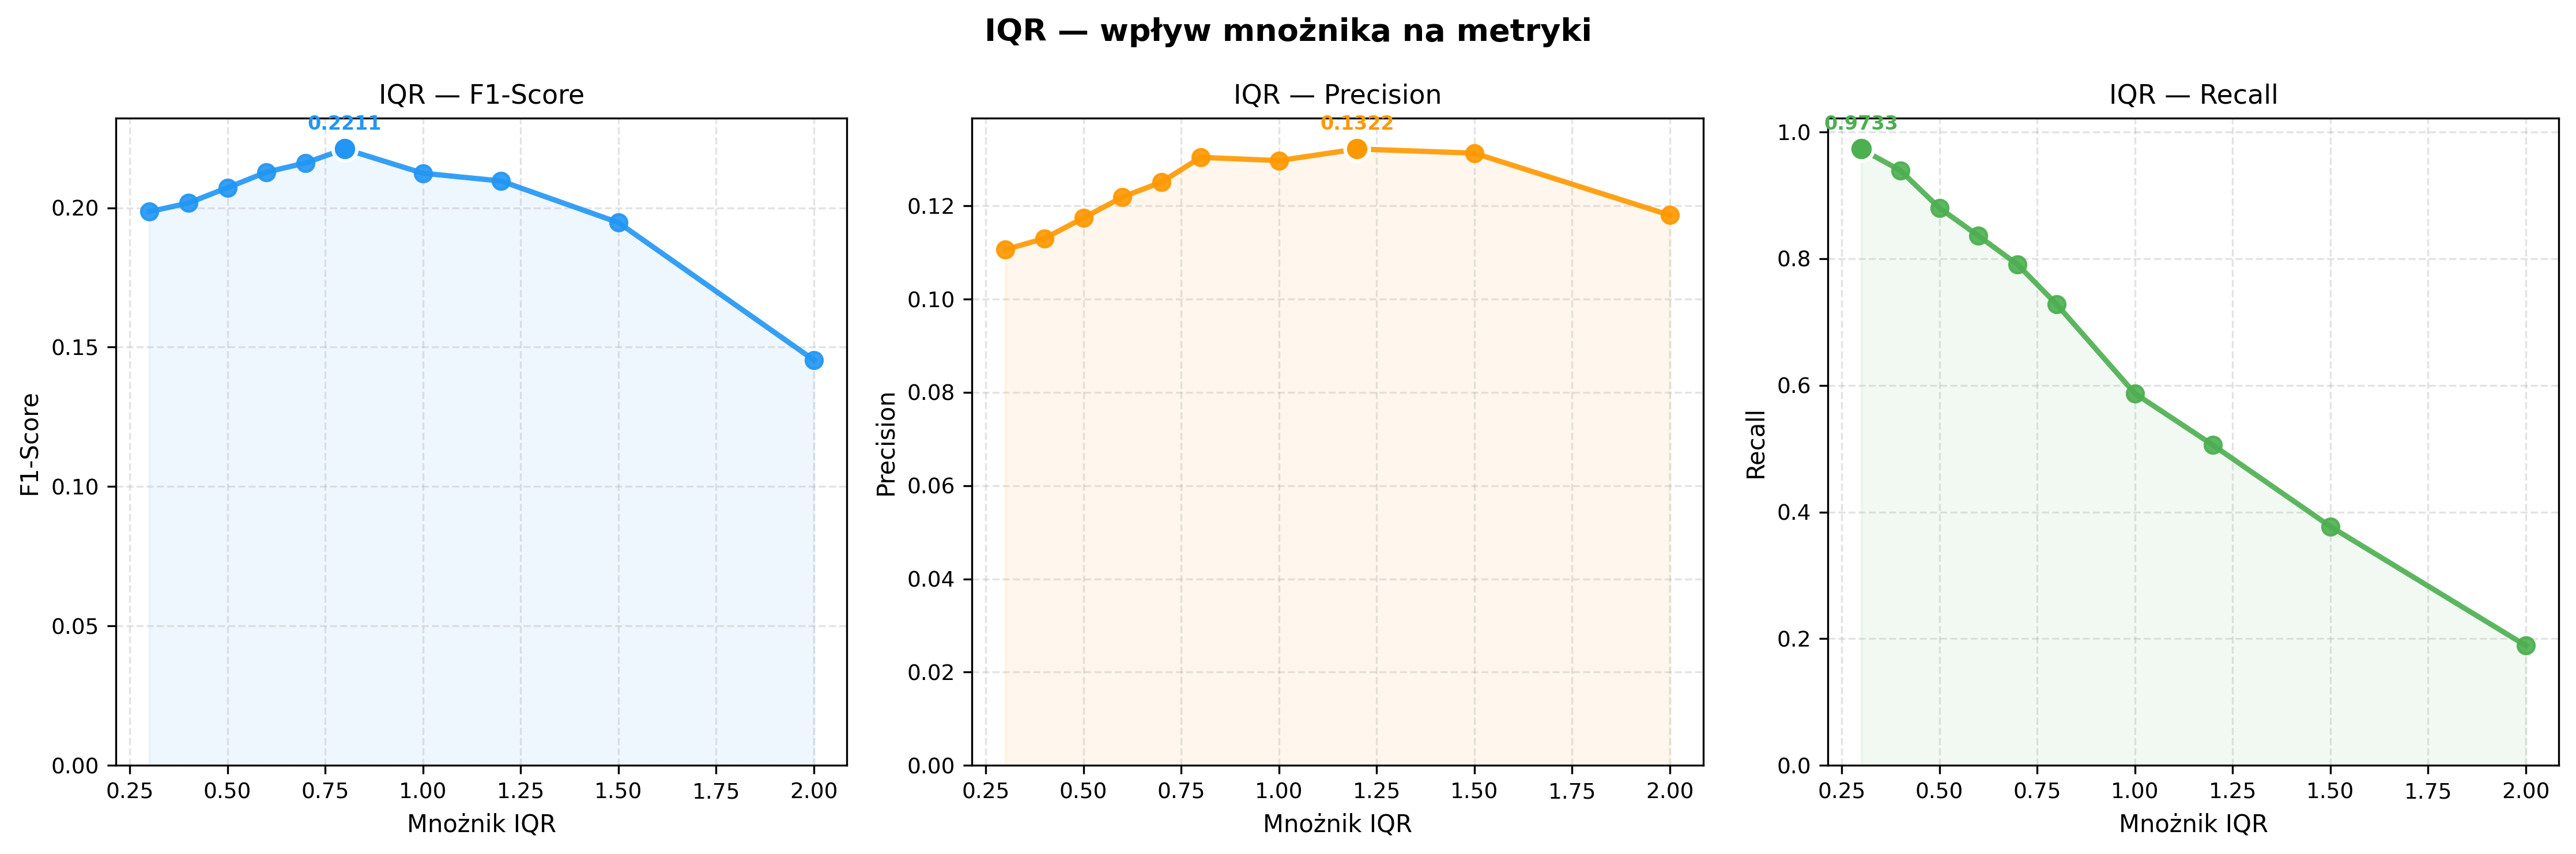
\includegraphics[width=0.9\textwidth]{fig_02b_iqr_params.png}
		\caption{Wpływ mnożnika na metryki detekcji w metodzie IQR}
		\label{fig:02b-iqr-params}
	\end{figure}
	
	\begin{figure}[H]
		\centering
		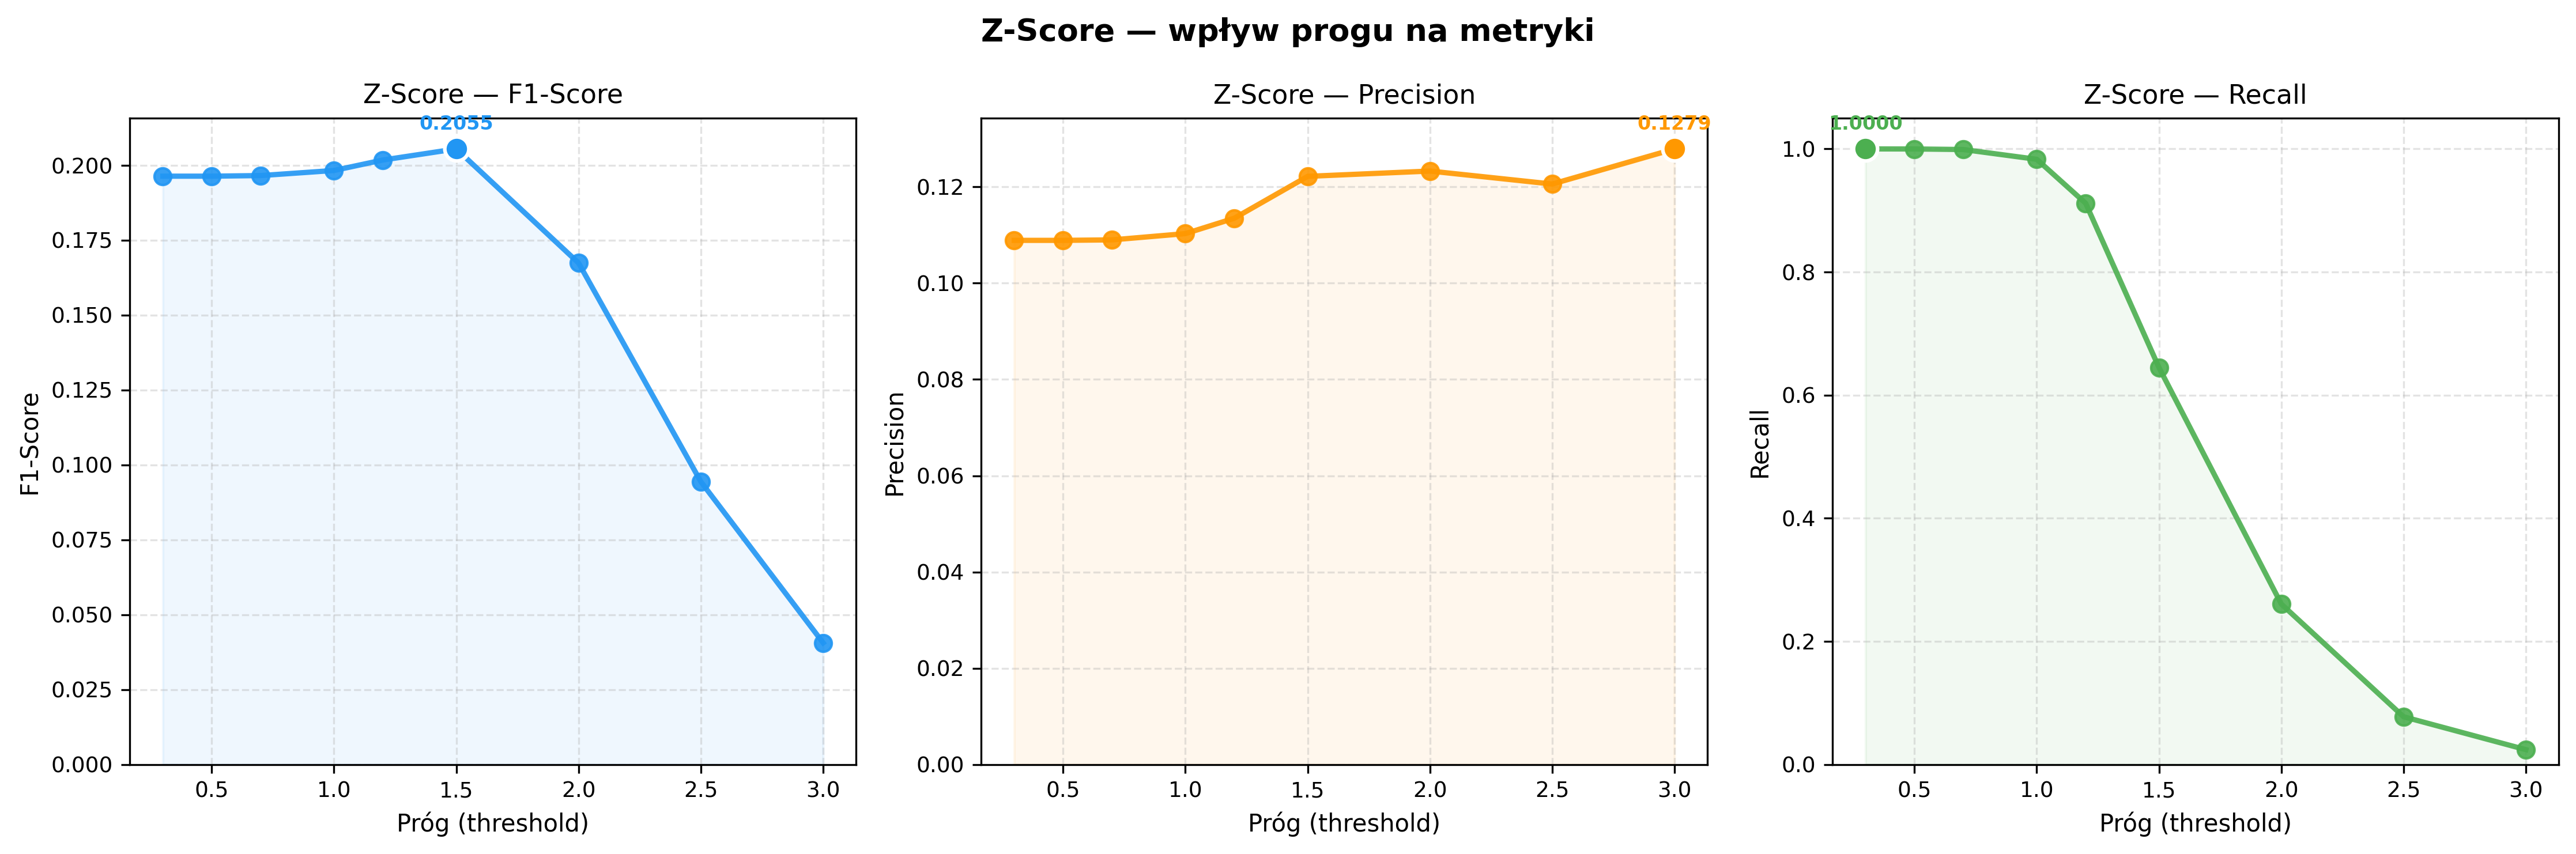
\includegraphics[width=0.9\textwidth]{fig_02b_zscore_params.png}
		\caption{Wpływ progu odcięcia na metryki detekcji w metodzie Z-Score}
		\label{fig:02b-zscore-params}
	\end{figure}
	
	
	\begin{figure}[H]
		\centering
		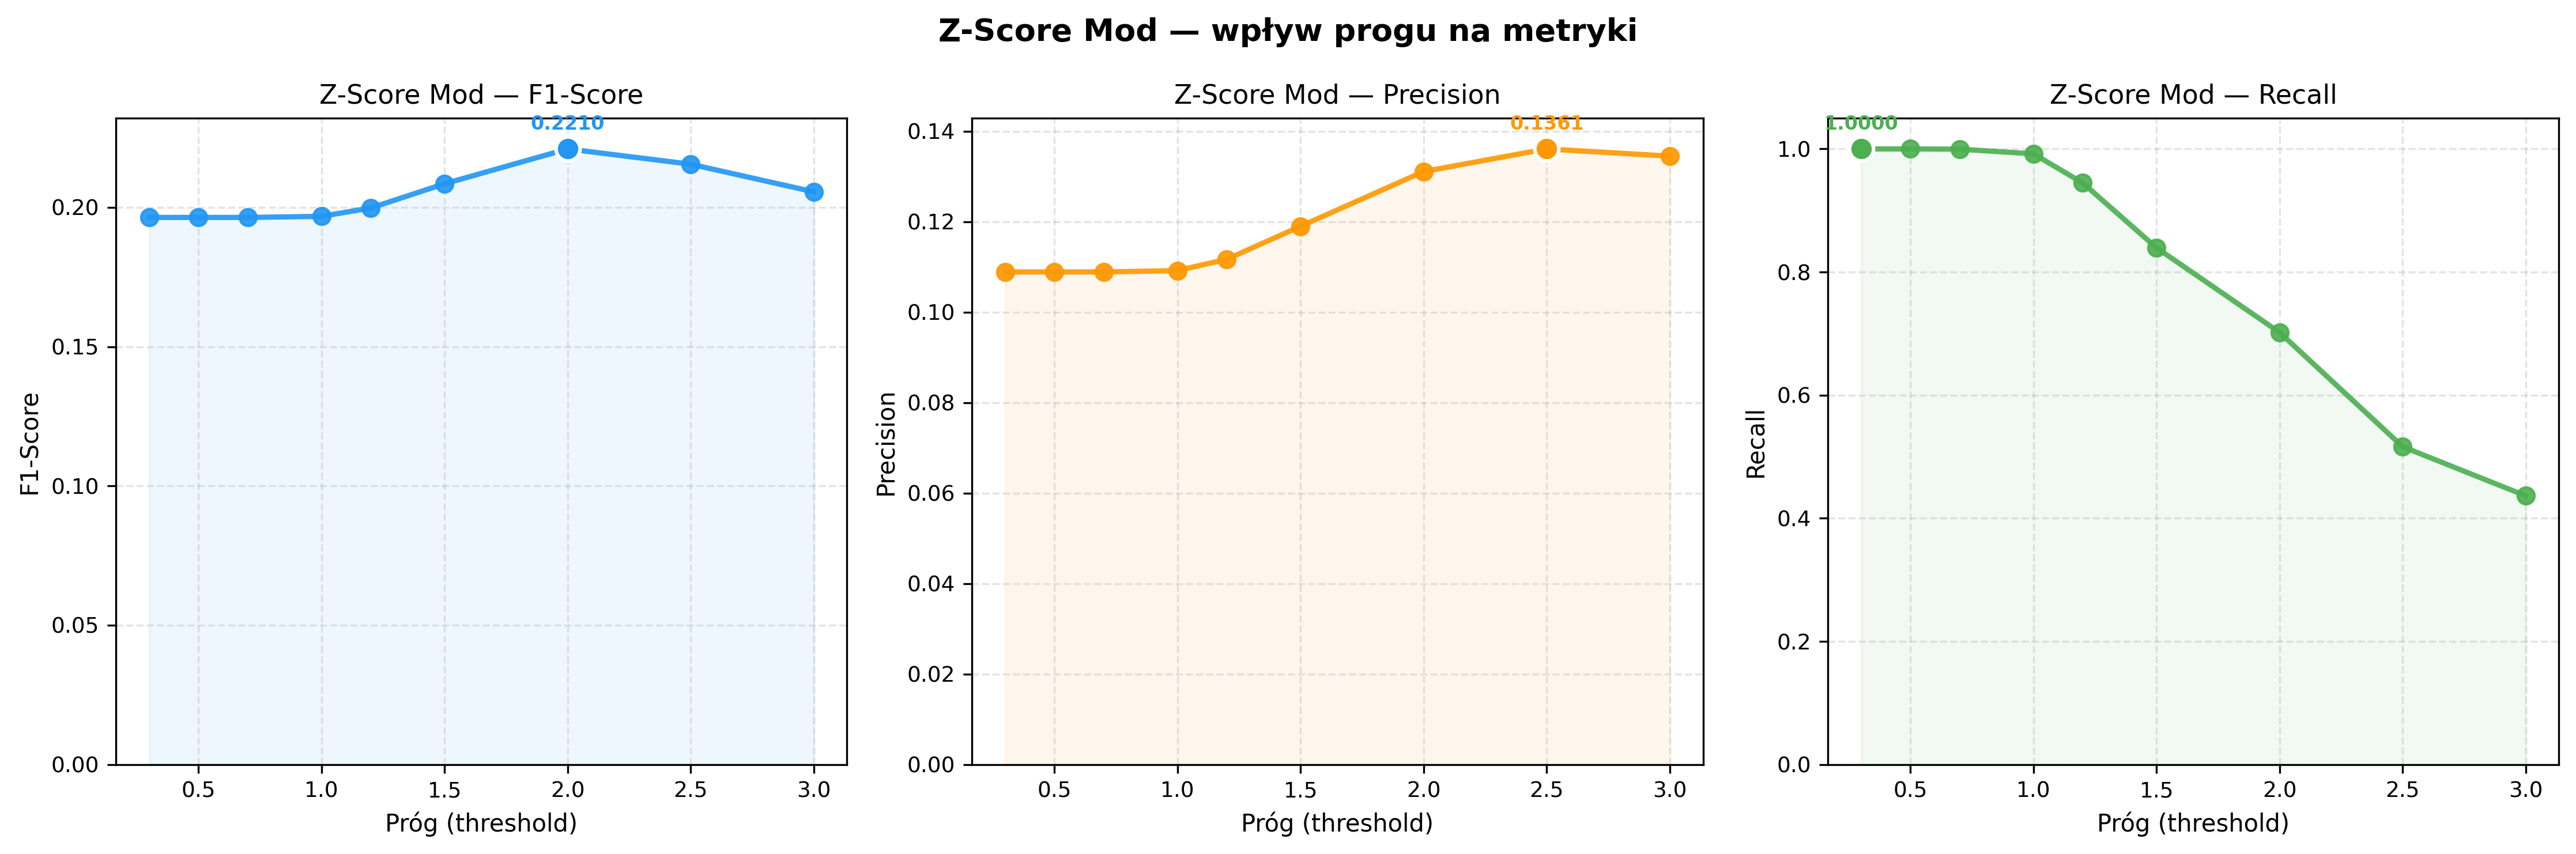
\includegraphics[width=0.9\textwidth]{fig_02b_zscore_mod_params.png}
		\caption{Wpływ progu odcięcia na metryki detekcji w zmodyfikowanej metodzie Z-Score}
		\label{fig:02b-zscore-mod-params}
	\end{figure}
	
	\begin{figure}[H]
		\centering
		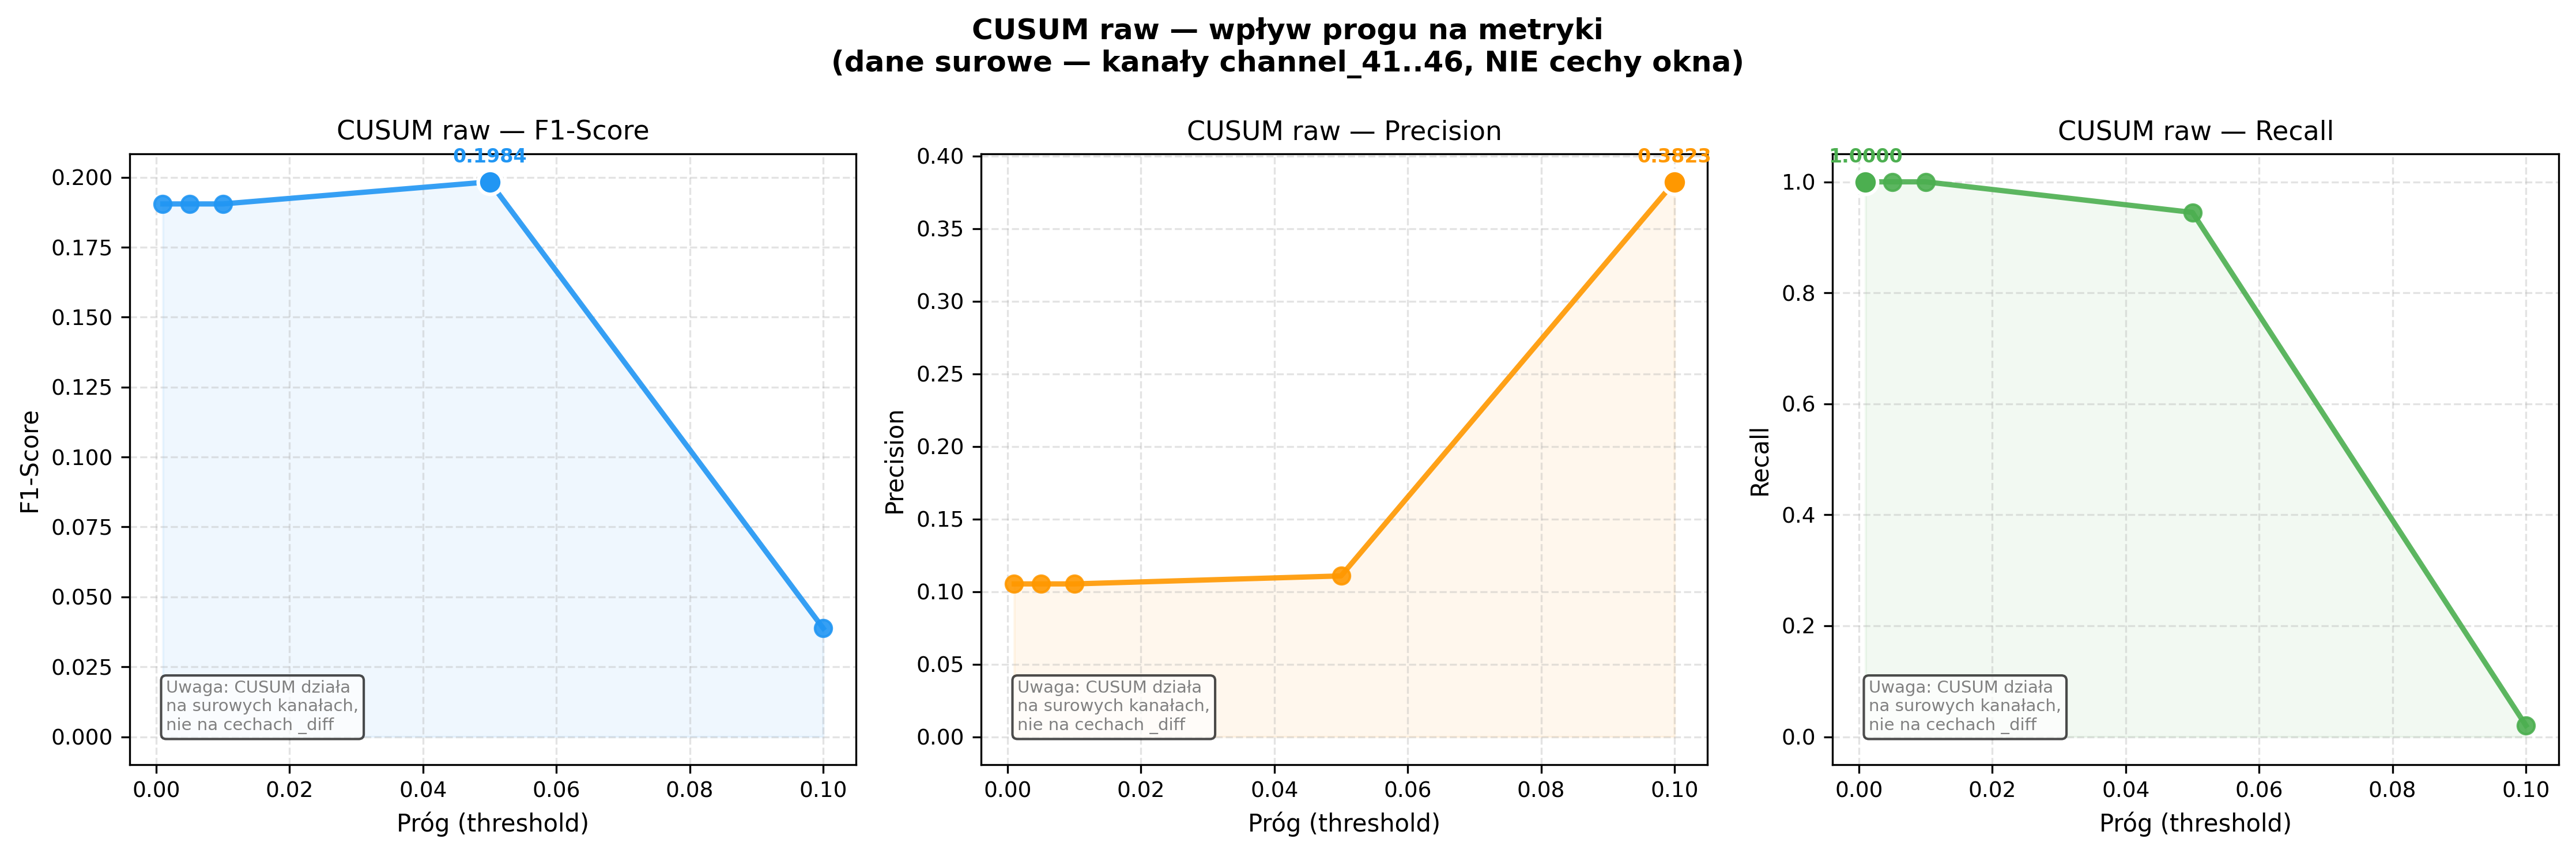
\includegraphics[width=0.9\textwidth]{fig_02b_cusum_raw_params.png}
		\caption{Wpływ progu detekcji na metryki w metodzie CUSUM na surowych danych.}
		\label{fig:02b-cusum_raw-params}
	\end{figure}
	
	\begin{figure}[H]
		\centering
		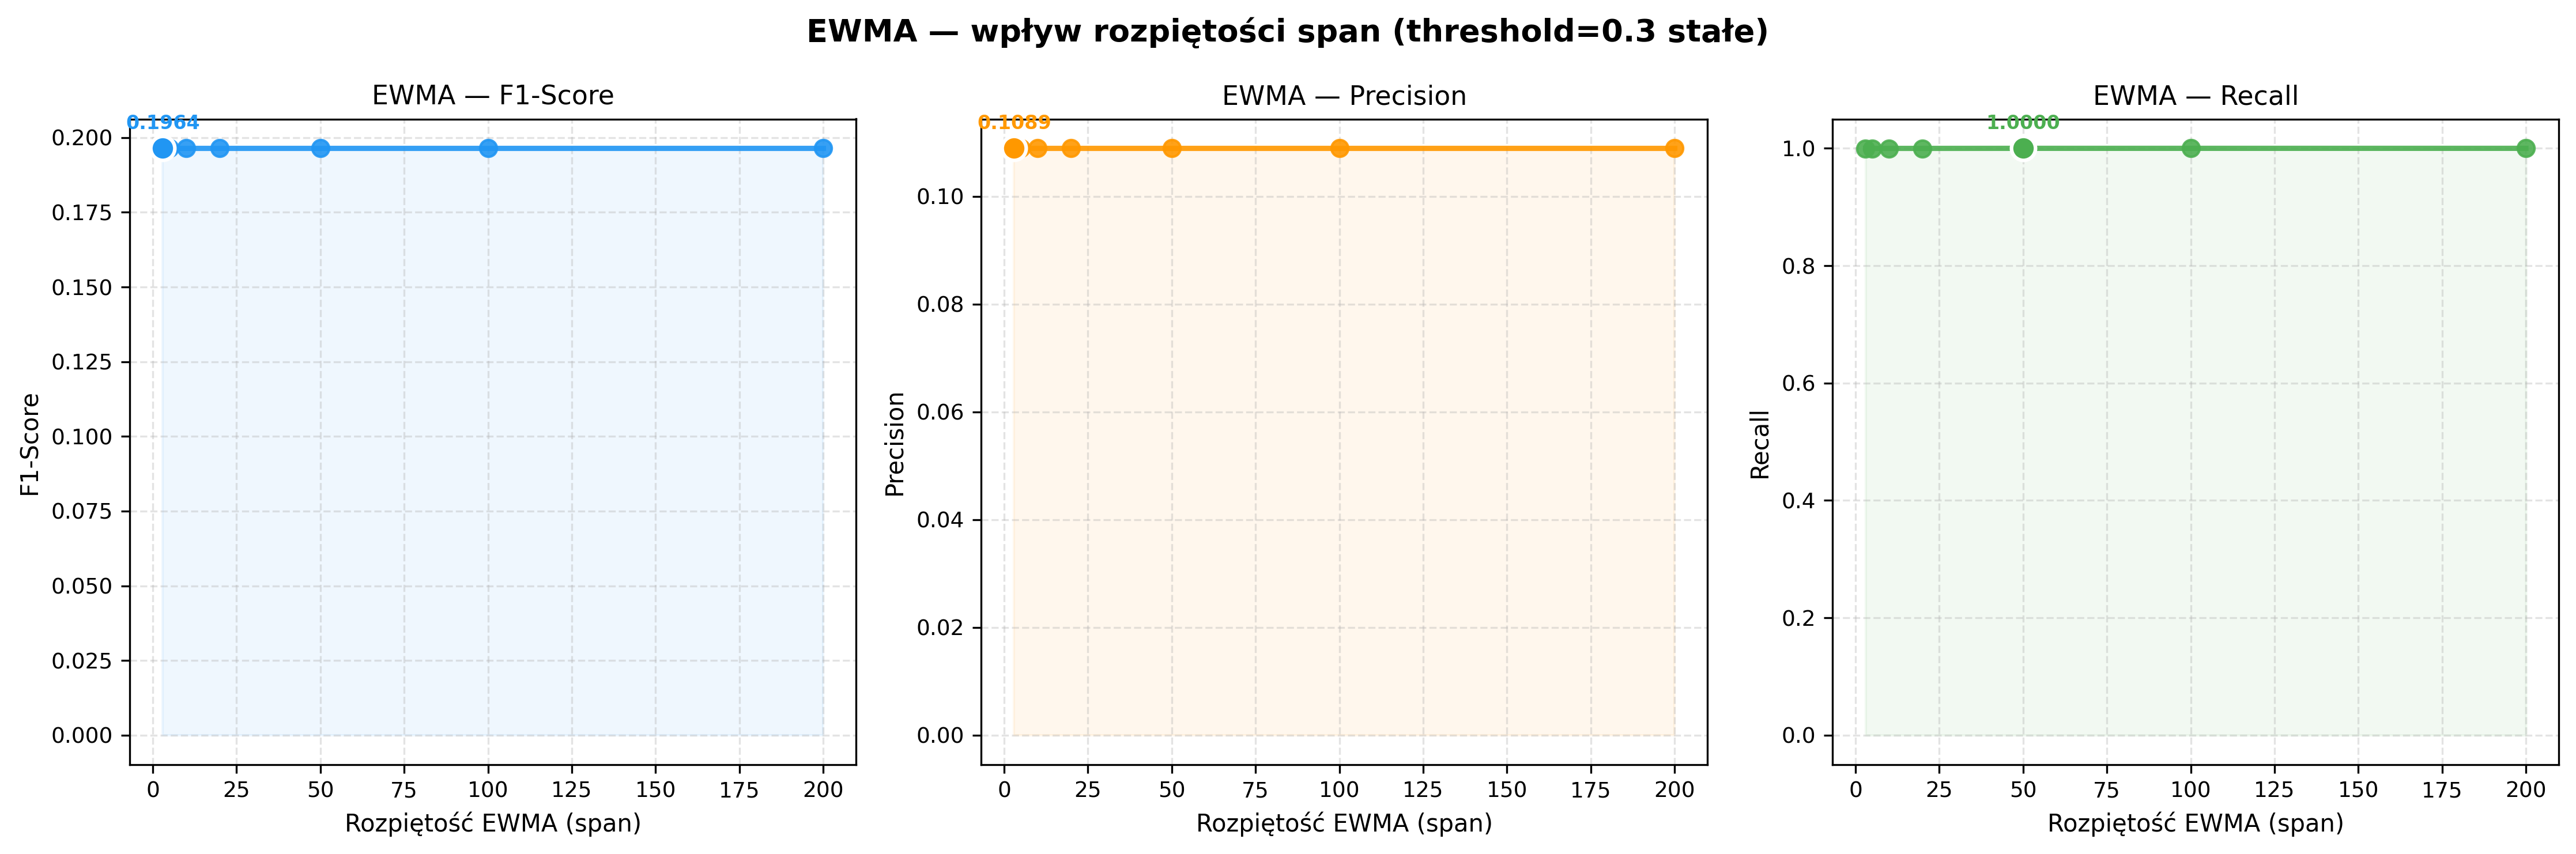
\includegraphics[width=0.9\textwidth]{fig_02b_ewma_span.png}
		\caption{Wpływ parametru rozpiętości na metryki w metodzie EWMA.}
		\label{fig:02b-ewma-span}
	\end{figure}
	
	\begin{figure}[H]
		\centering
		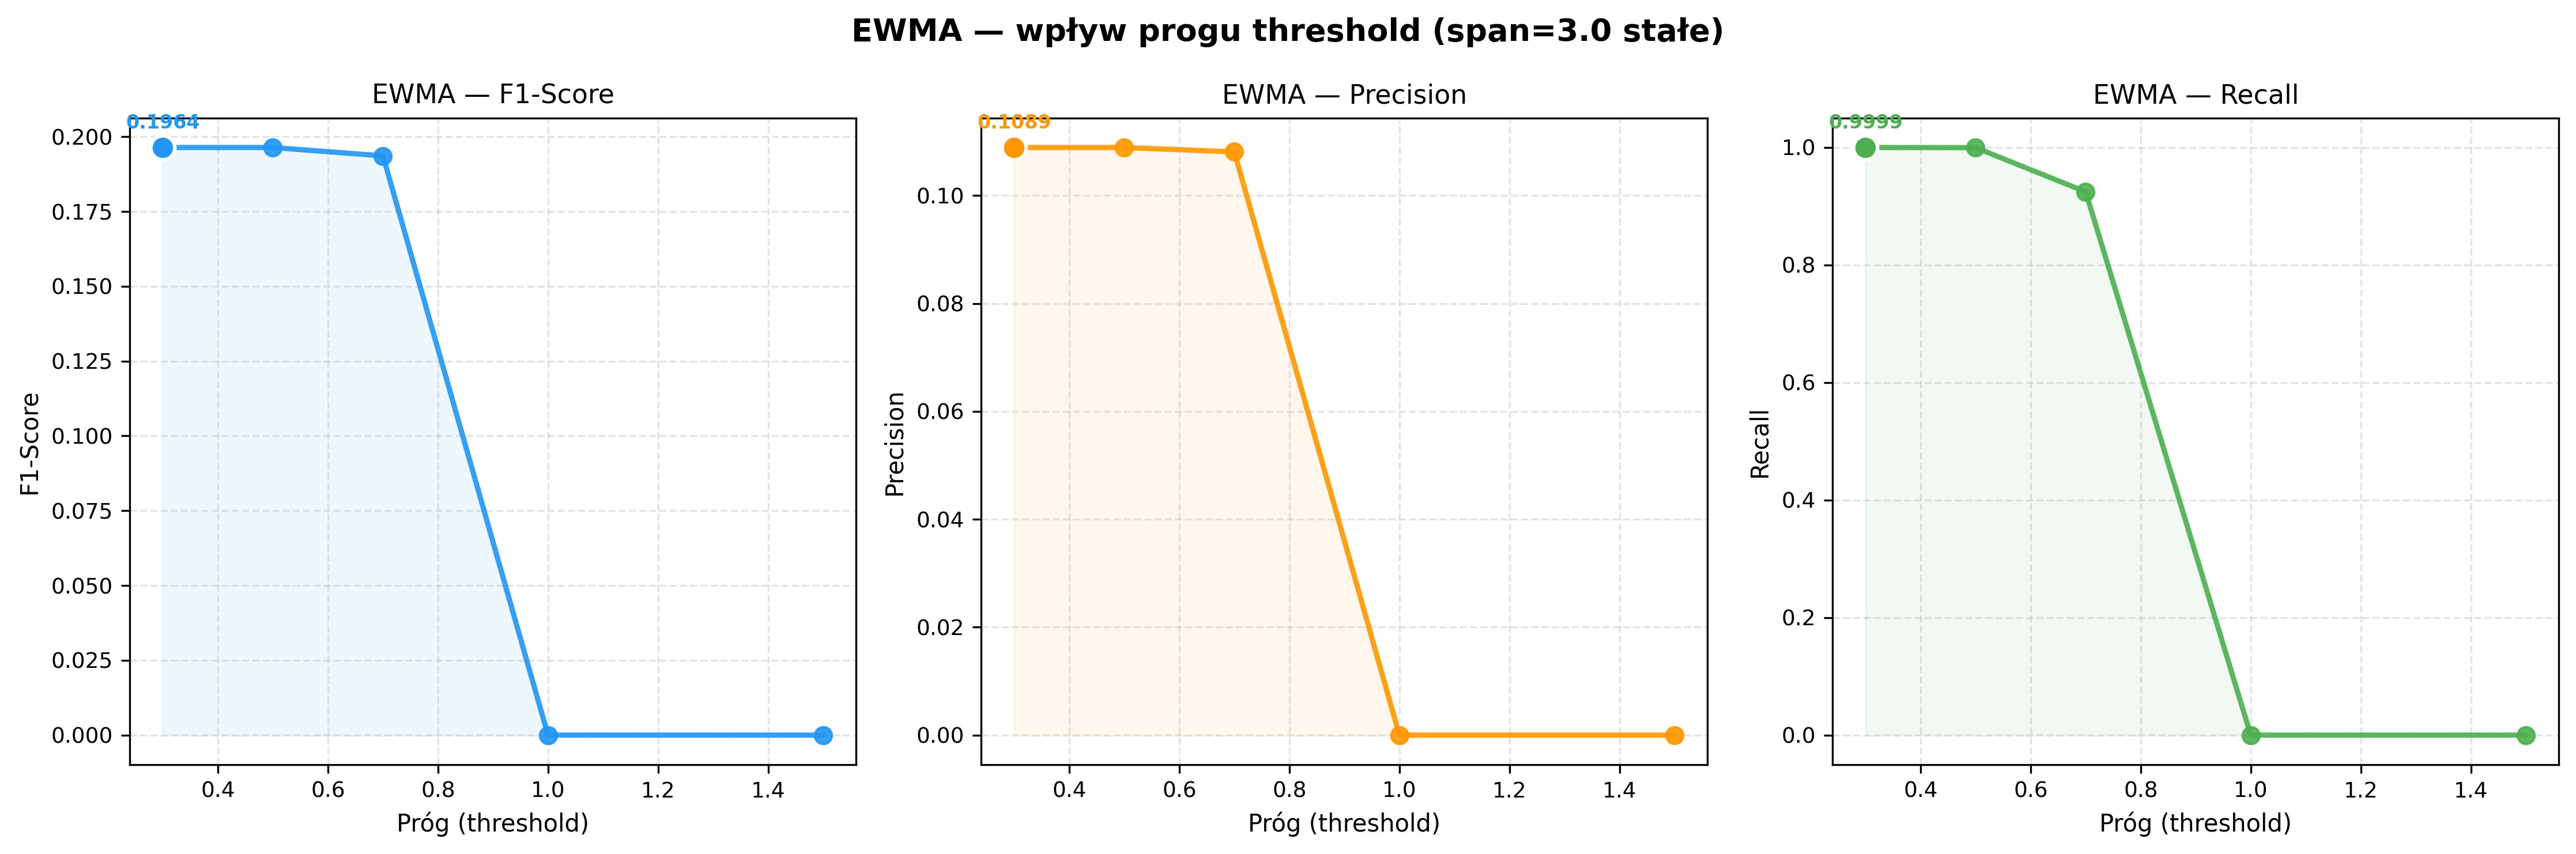
\includegraphics[width=0.9\textwidth]{fig_02b_ewma_threshold.png}
		\caption{Wpływ progu odcięcia na metryki w metodzie EWMA.}
		\label{fig:02b-ewma-threshold}
	\end{figure}
	
	\begin{figure}[H]
		\centering
		
\includegraphics[width=0.9\textwidth]{fig_02b_summary_comparison.png}
		\caption{Porównanie metryk uzyskanych przez metody statystyczne z pierwszym progiem}
		\label{fig:02b-summary-comparison}
	\end{figure}
	
	\section{Wyniki metod uczenia maszynowego}
	
	\begin{figure}[H]
		\centering
		
\includegraphics[width=0.9\textwidth]{fig_03b_if_params_v4.png}
		\caption{Wpływ parametru contamination(WIP) na metryki detekcji w algorytmie Isolation Forest}
		\label{fig:03b-if-params}
	\end{figure}
	
	\begin{figure}[H]
		\centering
		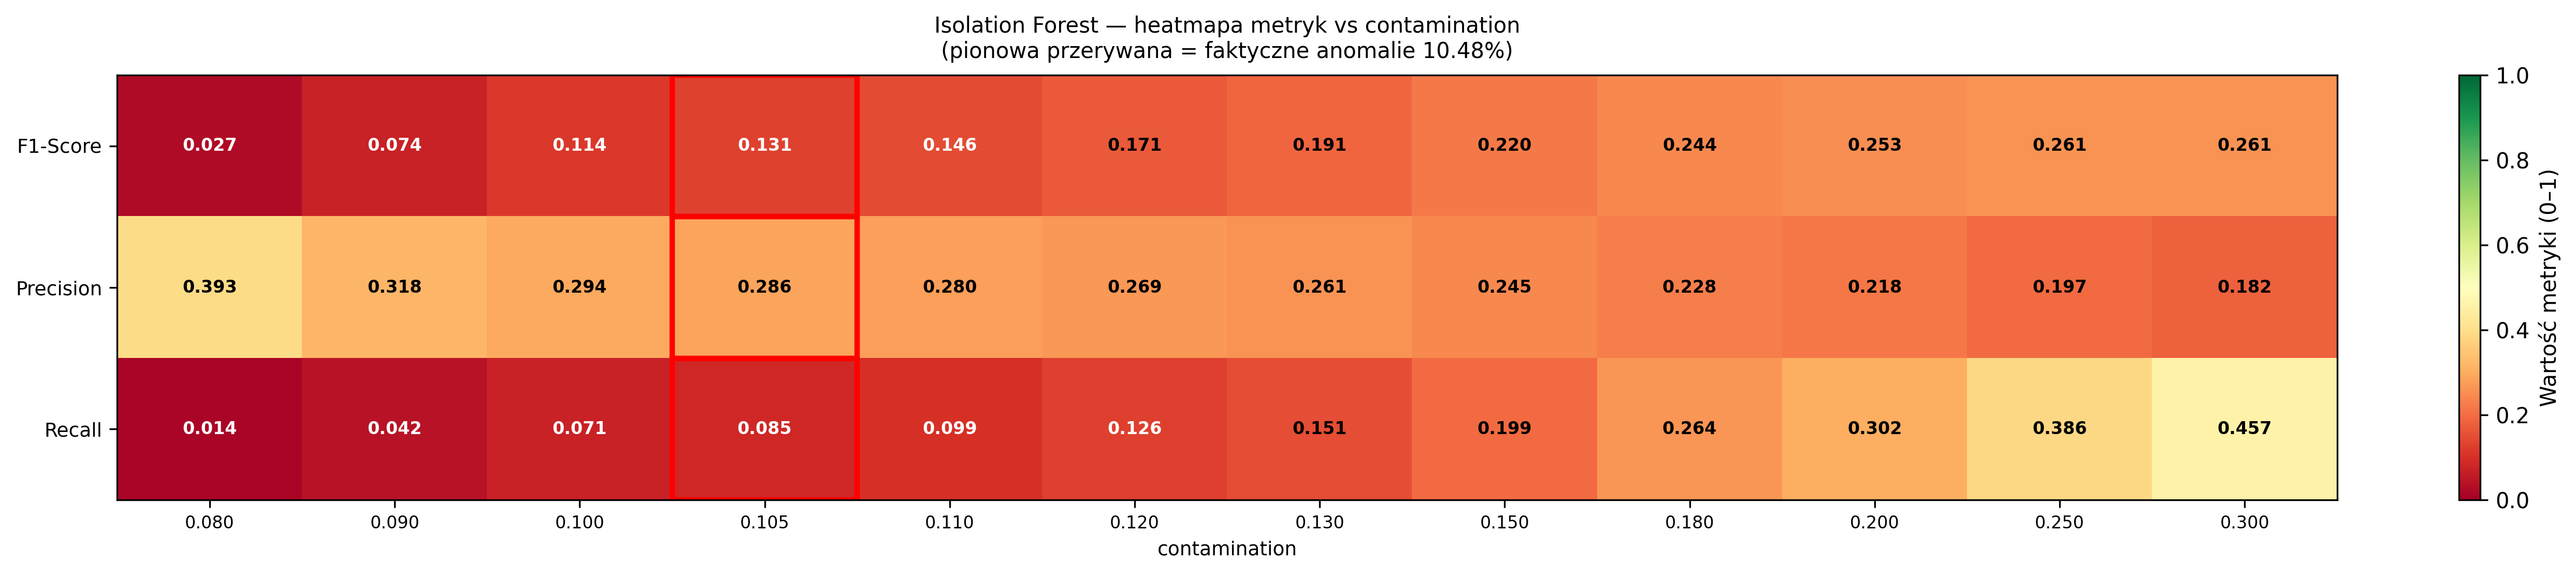
\includegraphics[width=0.9\textwidth]{fig_03b_isolation_forest_heatmap_v3.png}
		\caption{Macierz korelacji metryk z parametrem contamination(WIP) w algorytmie Isolation Forest}
		\label{fig:03b-isolation-forest-heatmap}
	\end{figure}
	
	\begin{figure}[H]
		\centering
		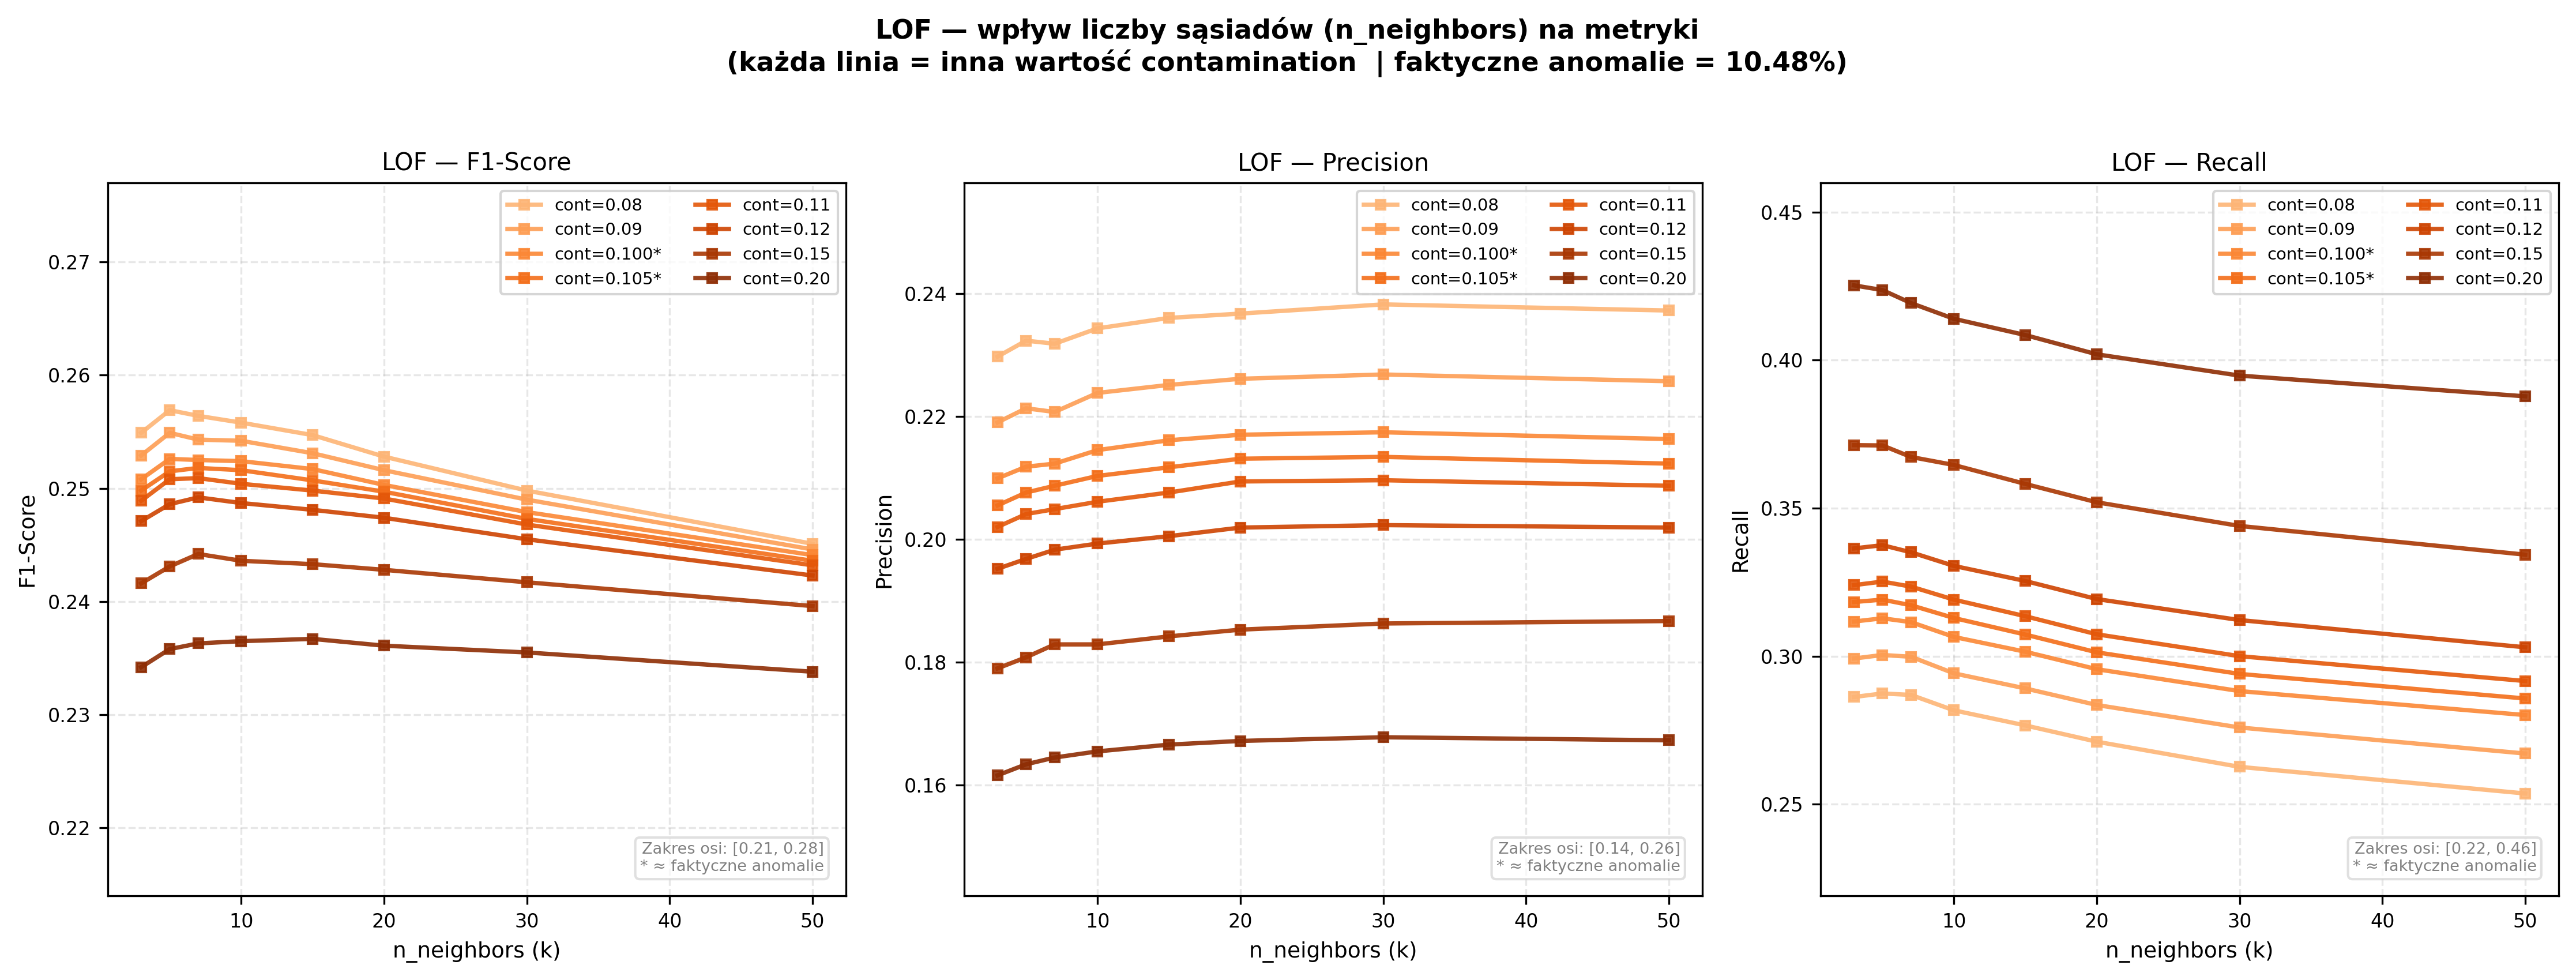
\includegraphics[width=0.9\textwidth]{fig_03b_lof_params_v4.png}
		\caption{Wpływ liczby sąsiadów na metryki detekcji w algorytmie Local Outlier Factor}
		\label{fig:03b-lof-params}
	\end{figure}
	
	\begin{figure}[H]
		\centering
		
\includegraphics[width=0.9\textwidth]{fig_03b_lof_heatmap_v3.png}
		\caption{Macierz korelacji metryk z parametrem contamination(WIP) w algorytmie Local Outlier Factor}
		\label{fig:03b-lof-heatmap}
	\end{figure}
	
	
	\begin{figure}[H]
		\centering
		
\includegraphics[width=0.9\textwidth]{fig_03b_svm_params_v4.png}
		\caption{Wpływ górnej granicy błędu na metryki decyzji w algorytmie One-Class SVM}
		\label{fig:03b-svm-mod-params}
	\end{figure}
	
	\begin{figure}[H]
		\centering
		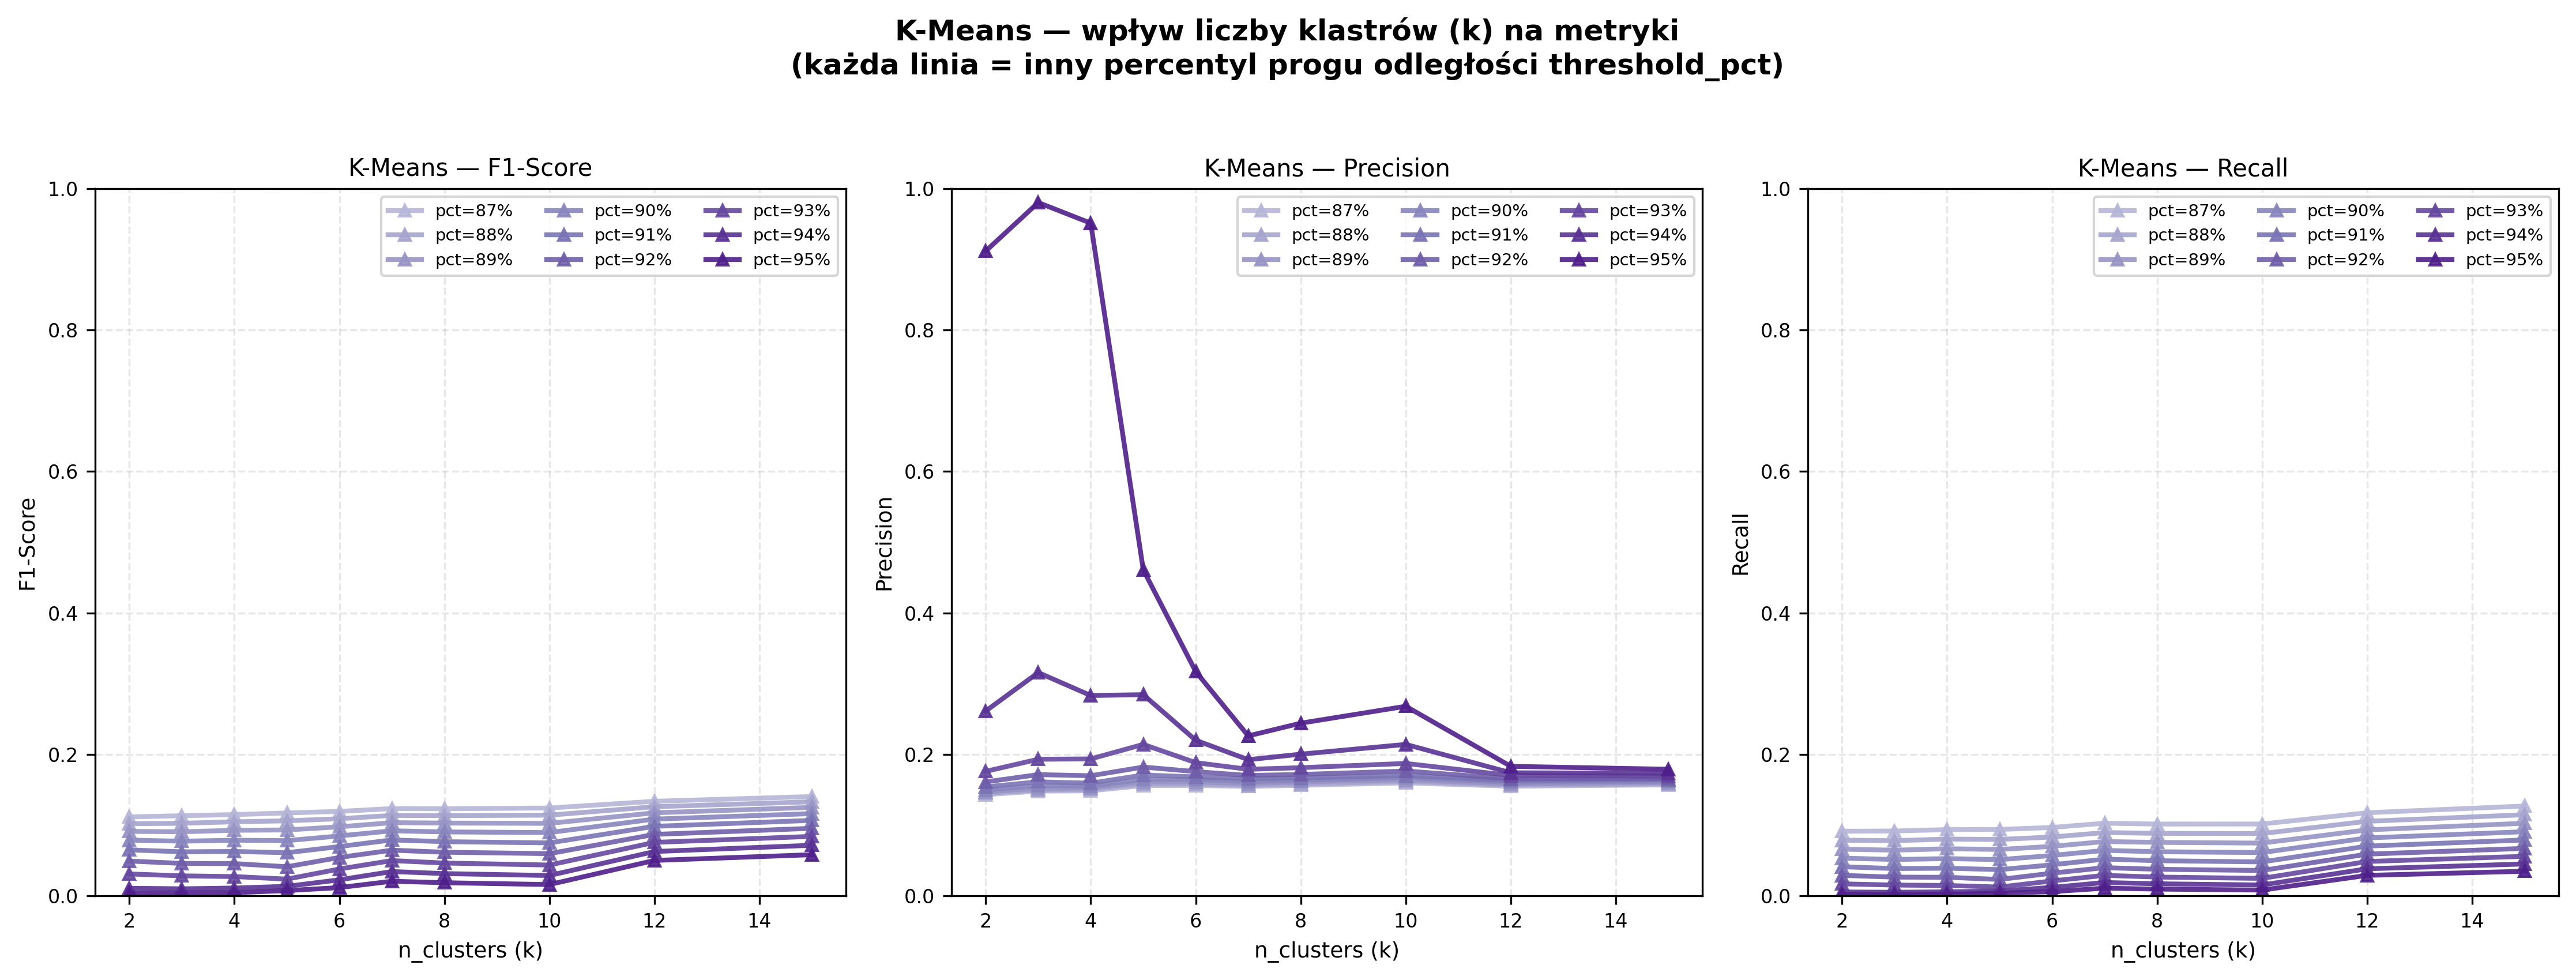
\includegraphics[width=0.9\textwidth]{fig_03b_kmeans_params_v3.png}
		\caption{Wpływ liczby klastrów na metryki detekcji w algorytmie K-Means}
		\label{fig:03b-kmeans-params}
	\end{figure}
	
	\begin{figure}[H]
		\centering
		
\includegraphics[width=0.9\textwidth]{fig_03b_kmeans_heatmap_v4.png}
		\caption{Macierz korelacji metryk z liczbą klastrów w algorytmie K-Means}
		\label{fig:03b-kmeans-heatmap}
	\end{figure}
	
	
	\begin{figure}[H]
		\centering
		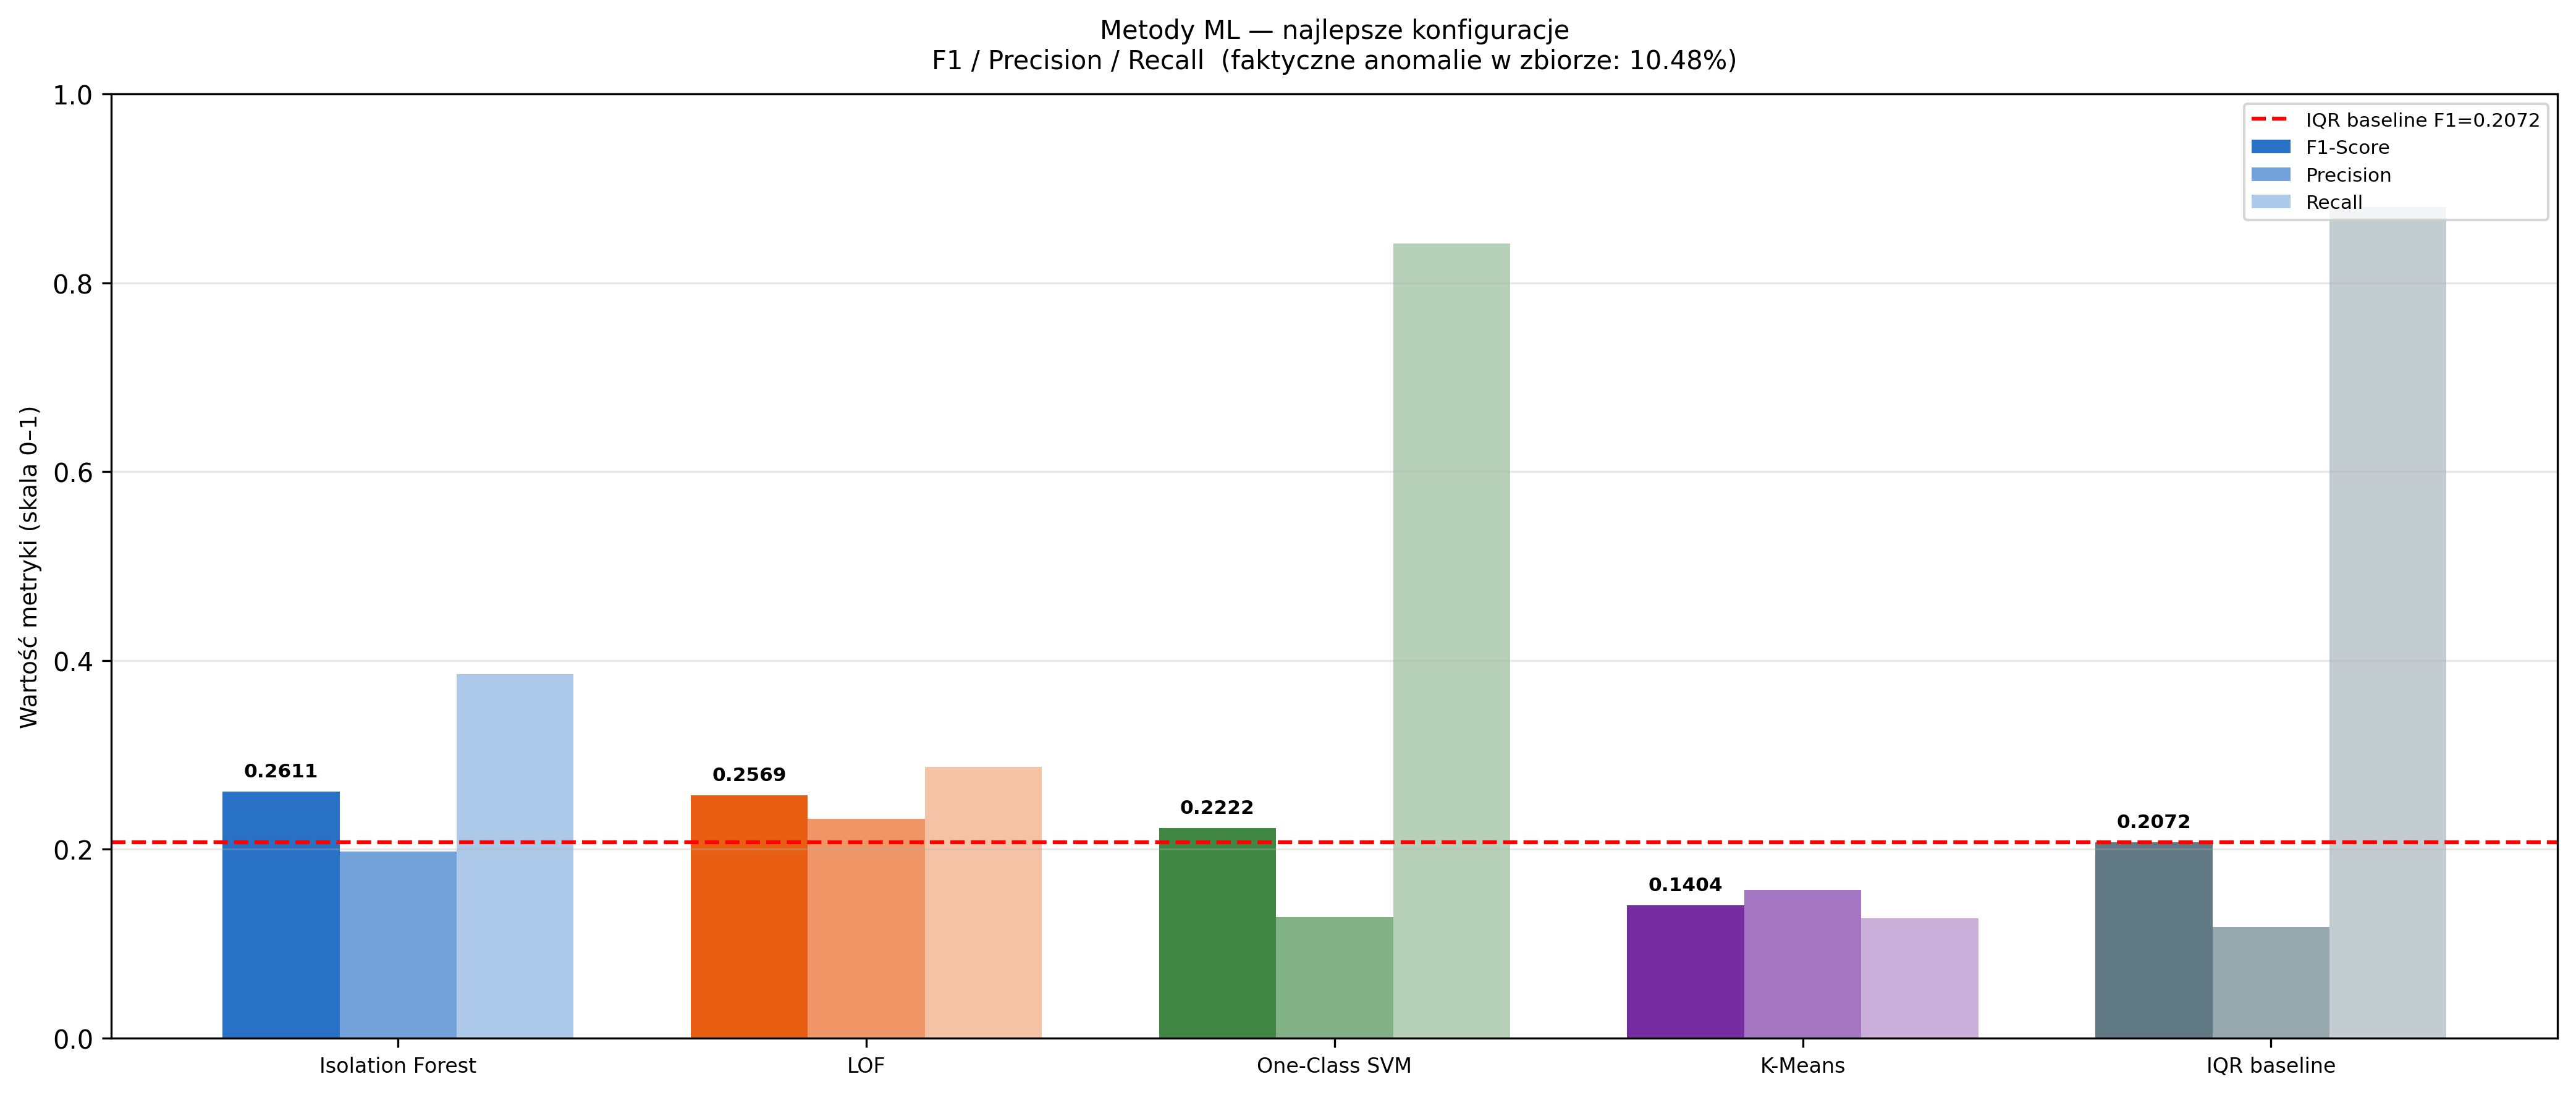
\includegraphics[width=0.9\textwidth]{fig_03b_summary_v4.png}
		\caption{Porównanie metryk uzyskanych przez metody uczenia maszynowego z pierwszym progiem}
		\label{fig:03b-summary}
	\end{figure}
	
	
	\section{Wyniki metod głębokiego uczenia i krzywe uczenia}
	
	\begin{figure}[H]
		\centering
		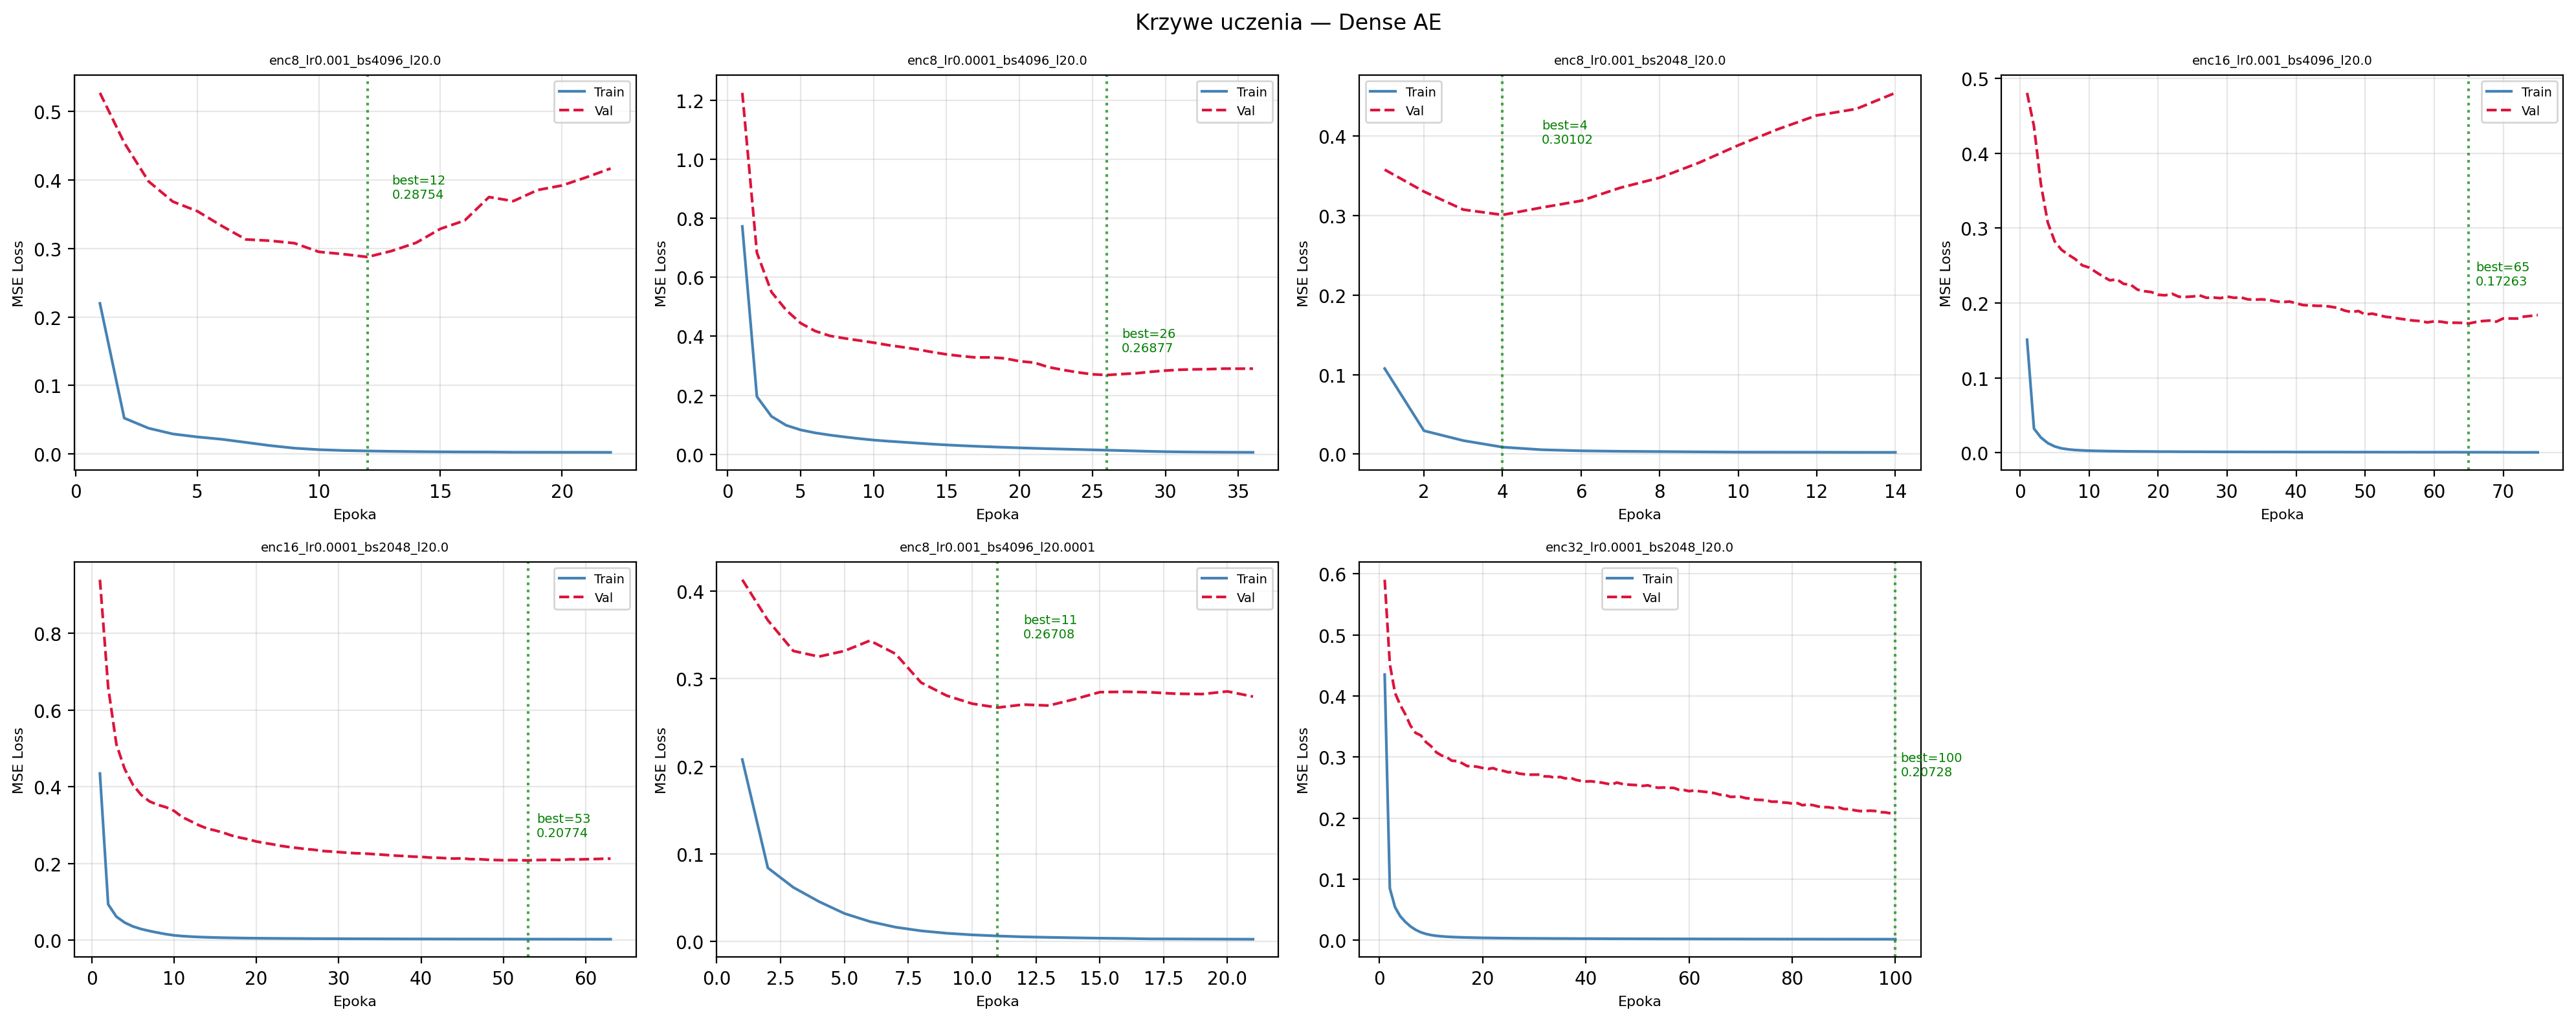
\includegraphics[width=0.9\textwidth]{fig_04b_curves_Dense_AE.png}
		\caption{Krzywe uczenia modelu sieci neuronowej w metodzie gęstej sieci neuronowej}
		\label{fig:04b-curves-dense}
	\end{figure}
	
	\begin{figure}[H]
		\centering
		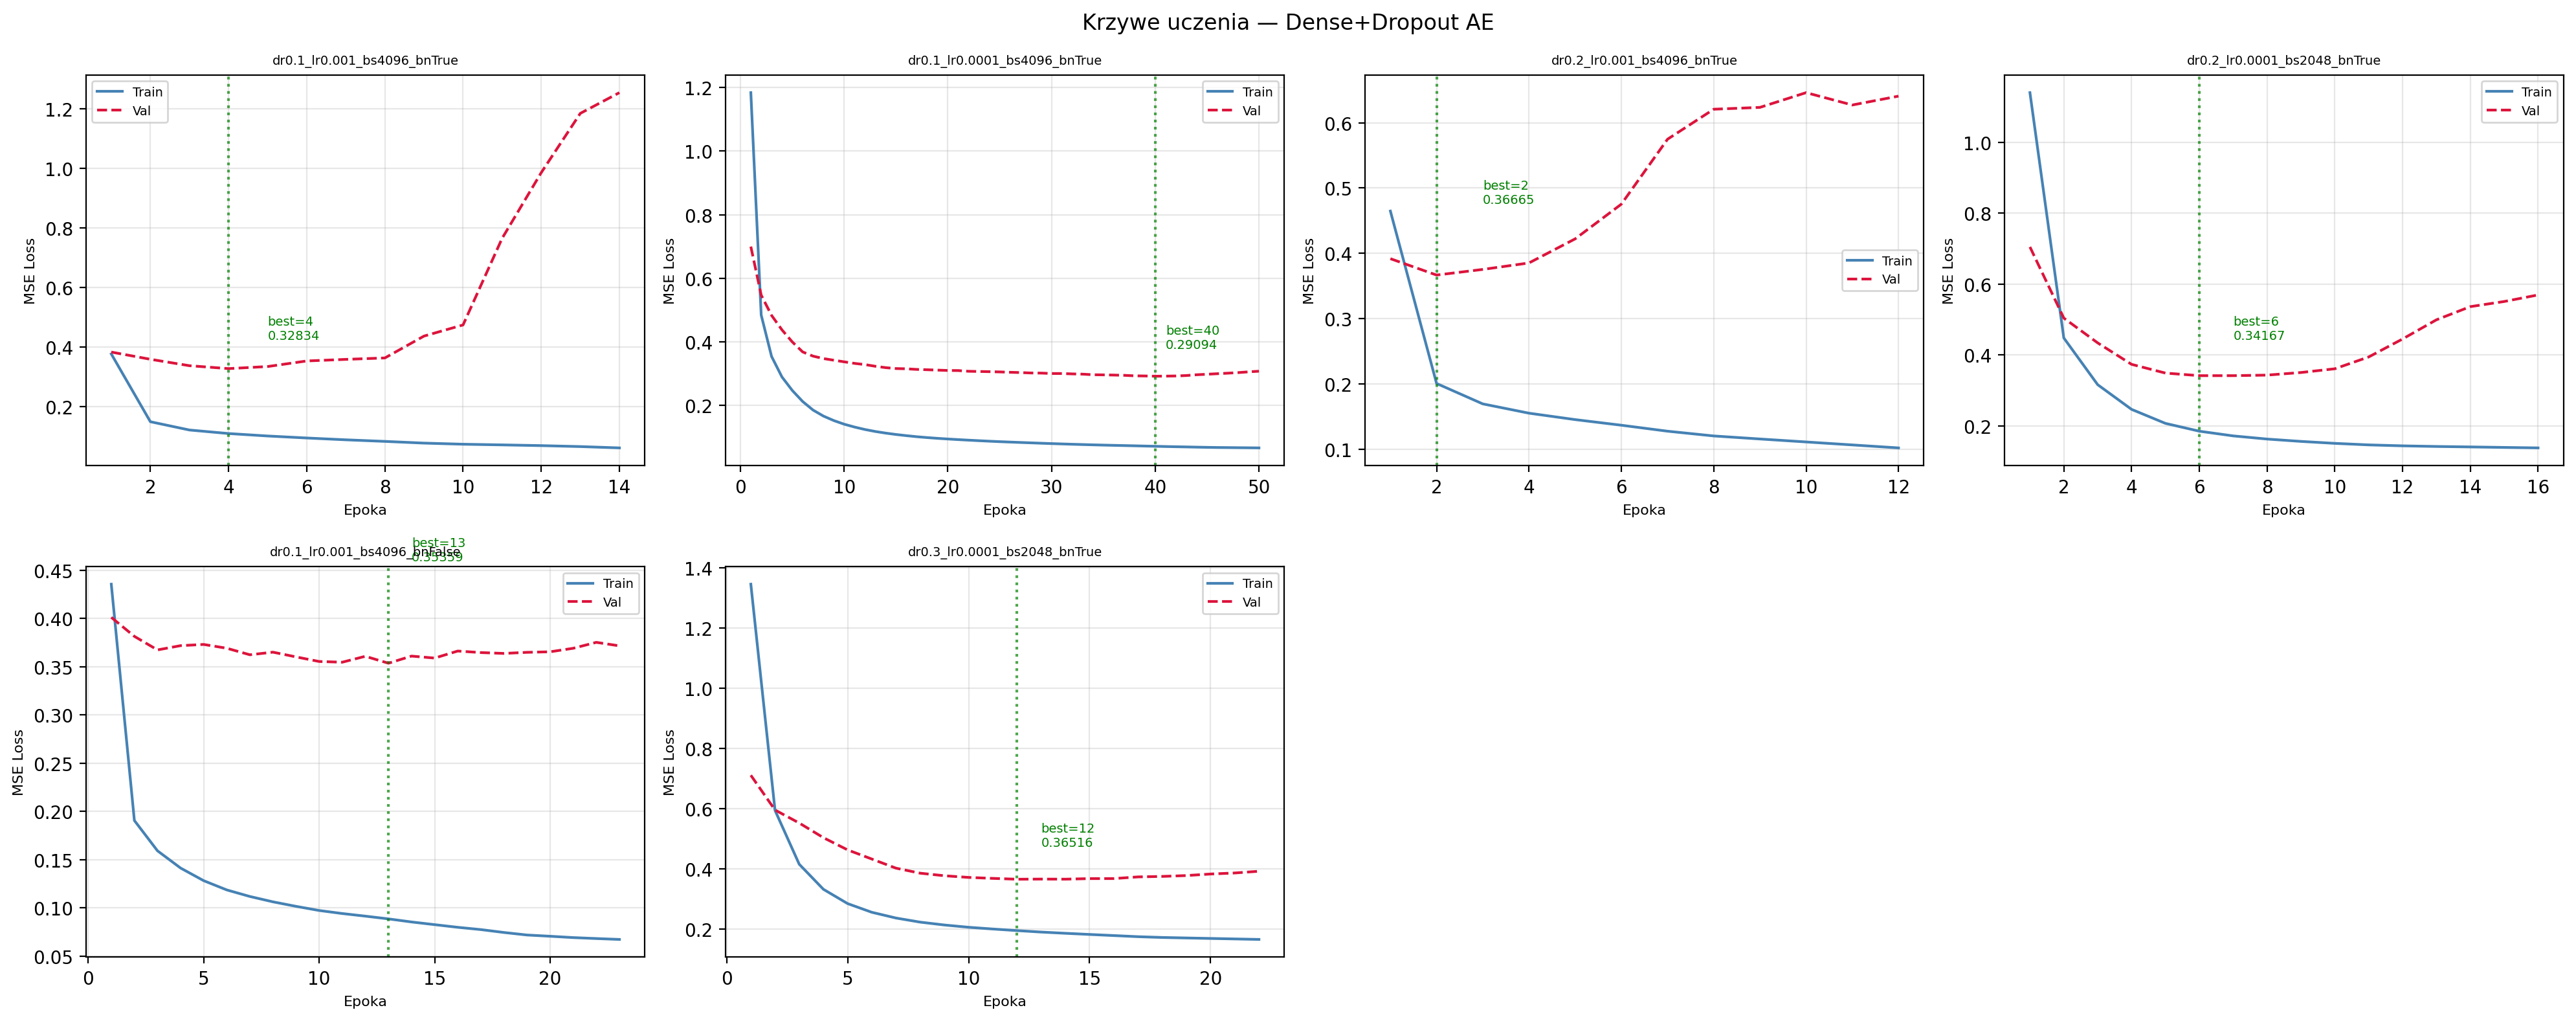
\includegraphics[width=0.9\textwidth]{fig_04b_curves_Dense+Dropout_AE.png}
		\caption{Krzywe uczenia modelu sieci neuronowej w metodzie gęstej sieci neuronowej z droputem}
		\label{fig:04b-curves-dense-dropout}
	\end{figure}
	
	\begin{figure}[H]
		\centering
		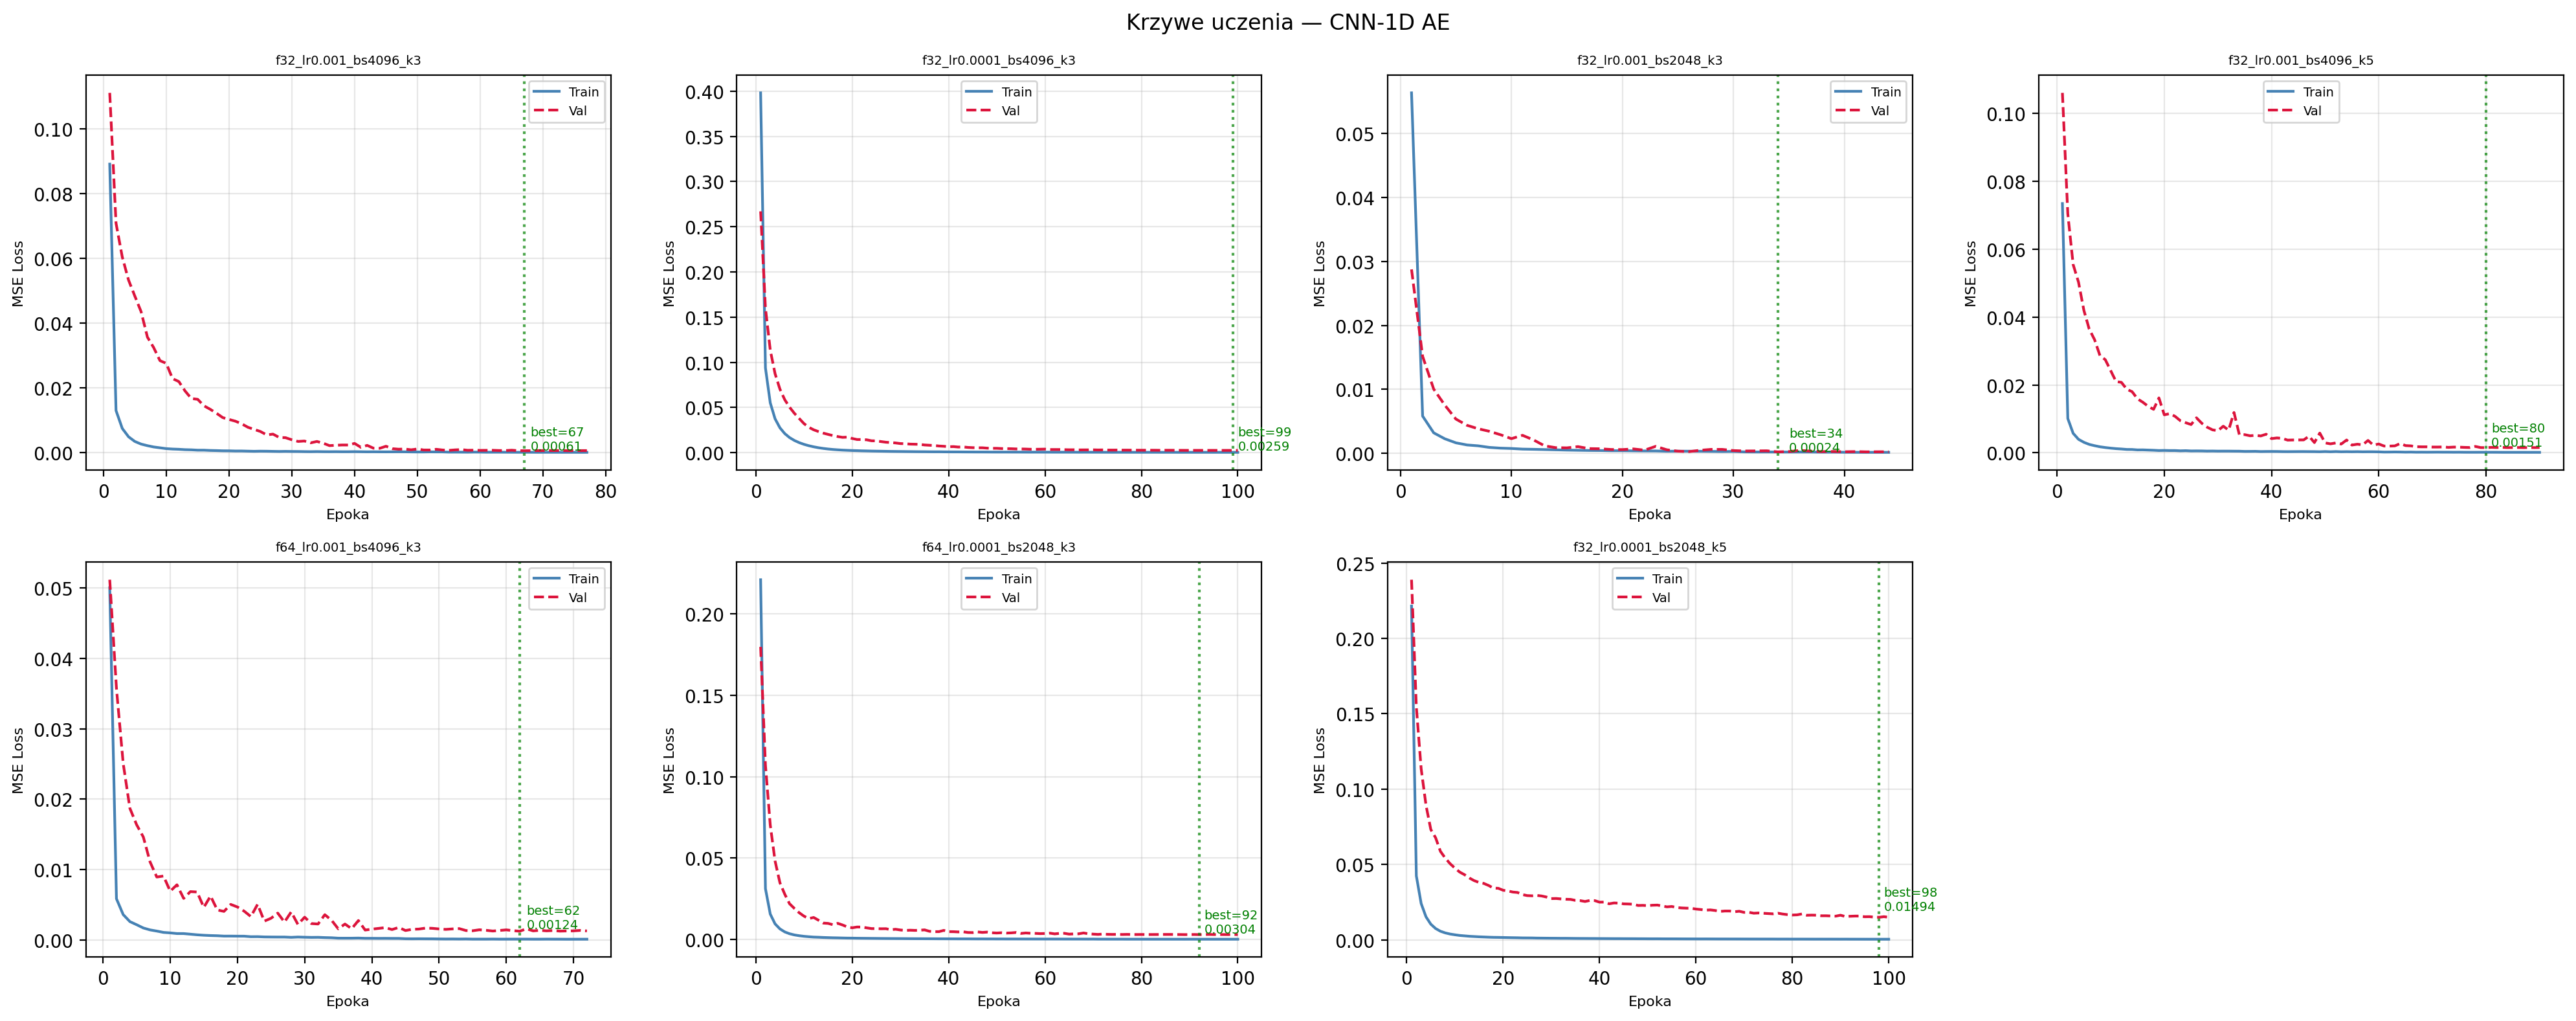
\includegraphics[width=0.9\textwidth]{fig_04b_curves_CNN-1D_AE.png}
		\caption{Krzywe uczenia modelu sieci neuronowej w metodzie konwolucyjnej sieci neuronowej}
		\label{fig:04b-curves-cnn1d}
	\end{figure}
	
	\begin{figure}[H]
		\centering
		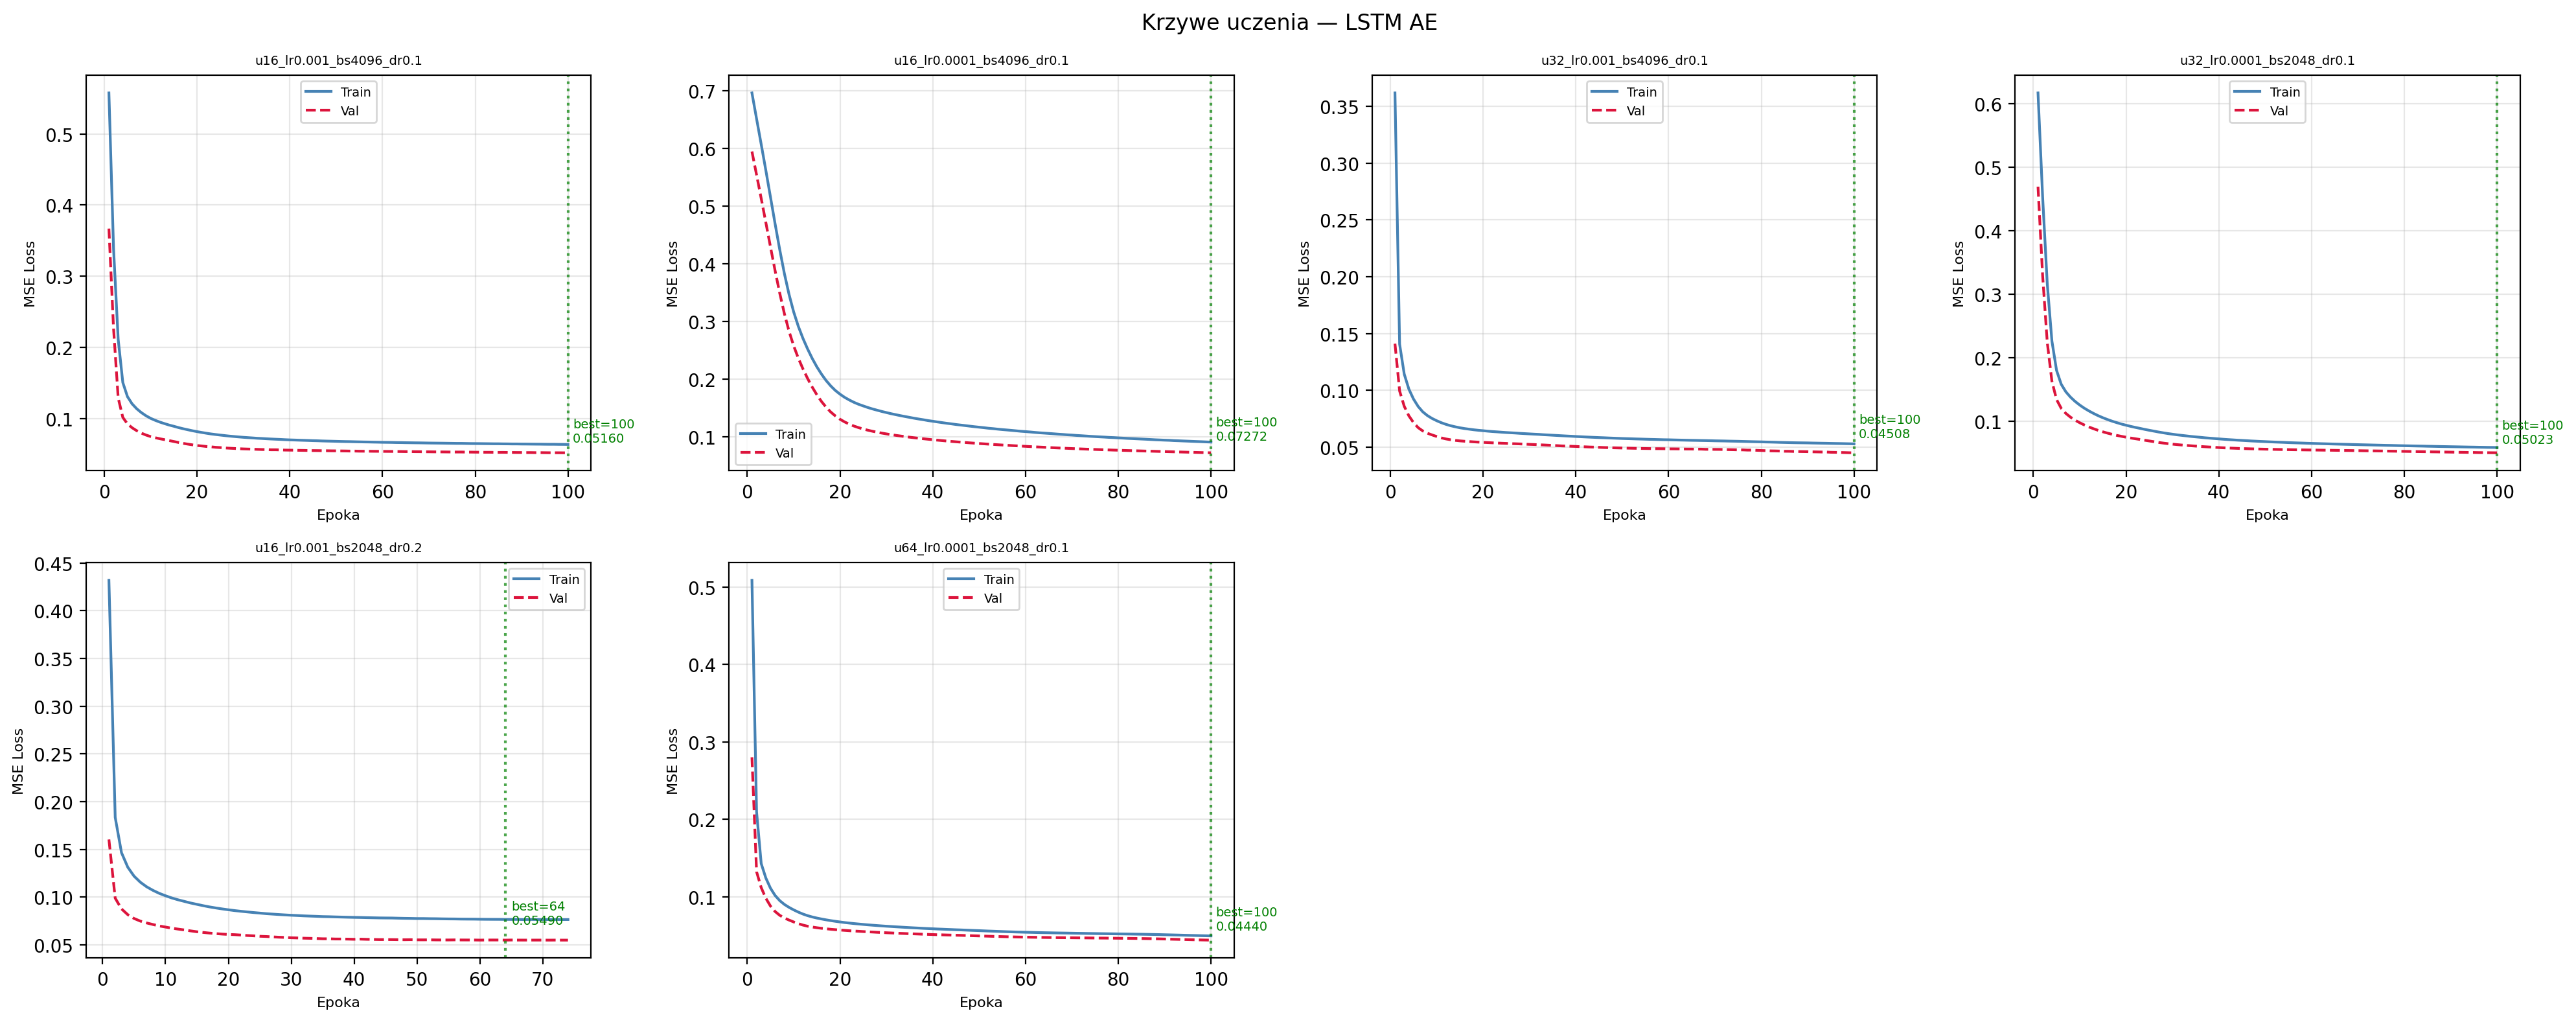
\includegraphics[width=0.9\textwidth]{fig_04b_curves_LSTM_AE.png}
		\caption{Krzywe uczenia modelu sieci neuronowej w metodzie rekurencyjnej sieci neuronowej}
		\label{fig:04b-curves-lstm}
	\end{figure}
	
	\begin{figure}[H]
		\centering
		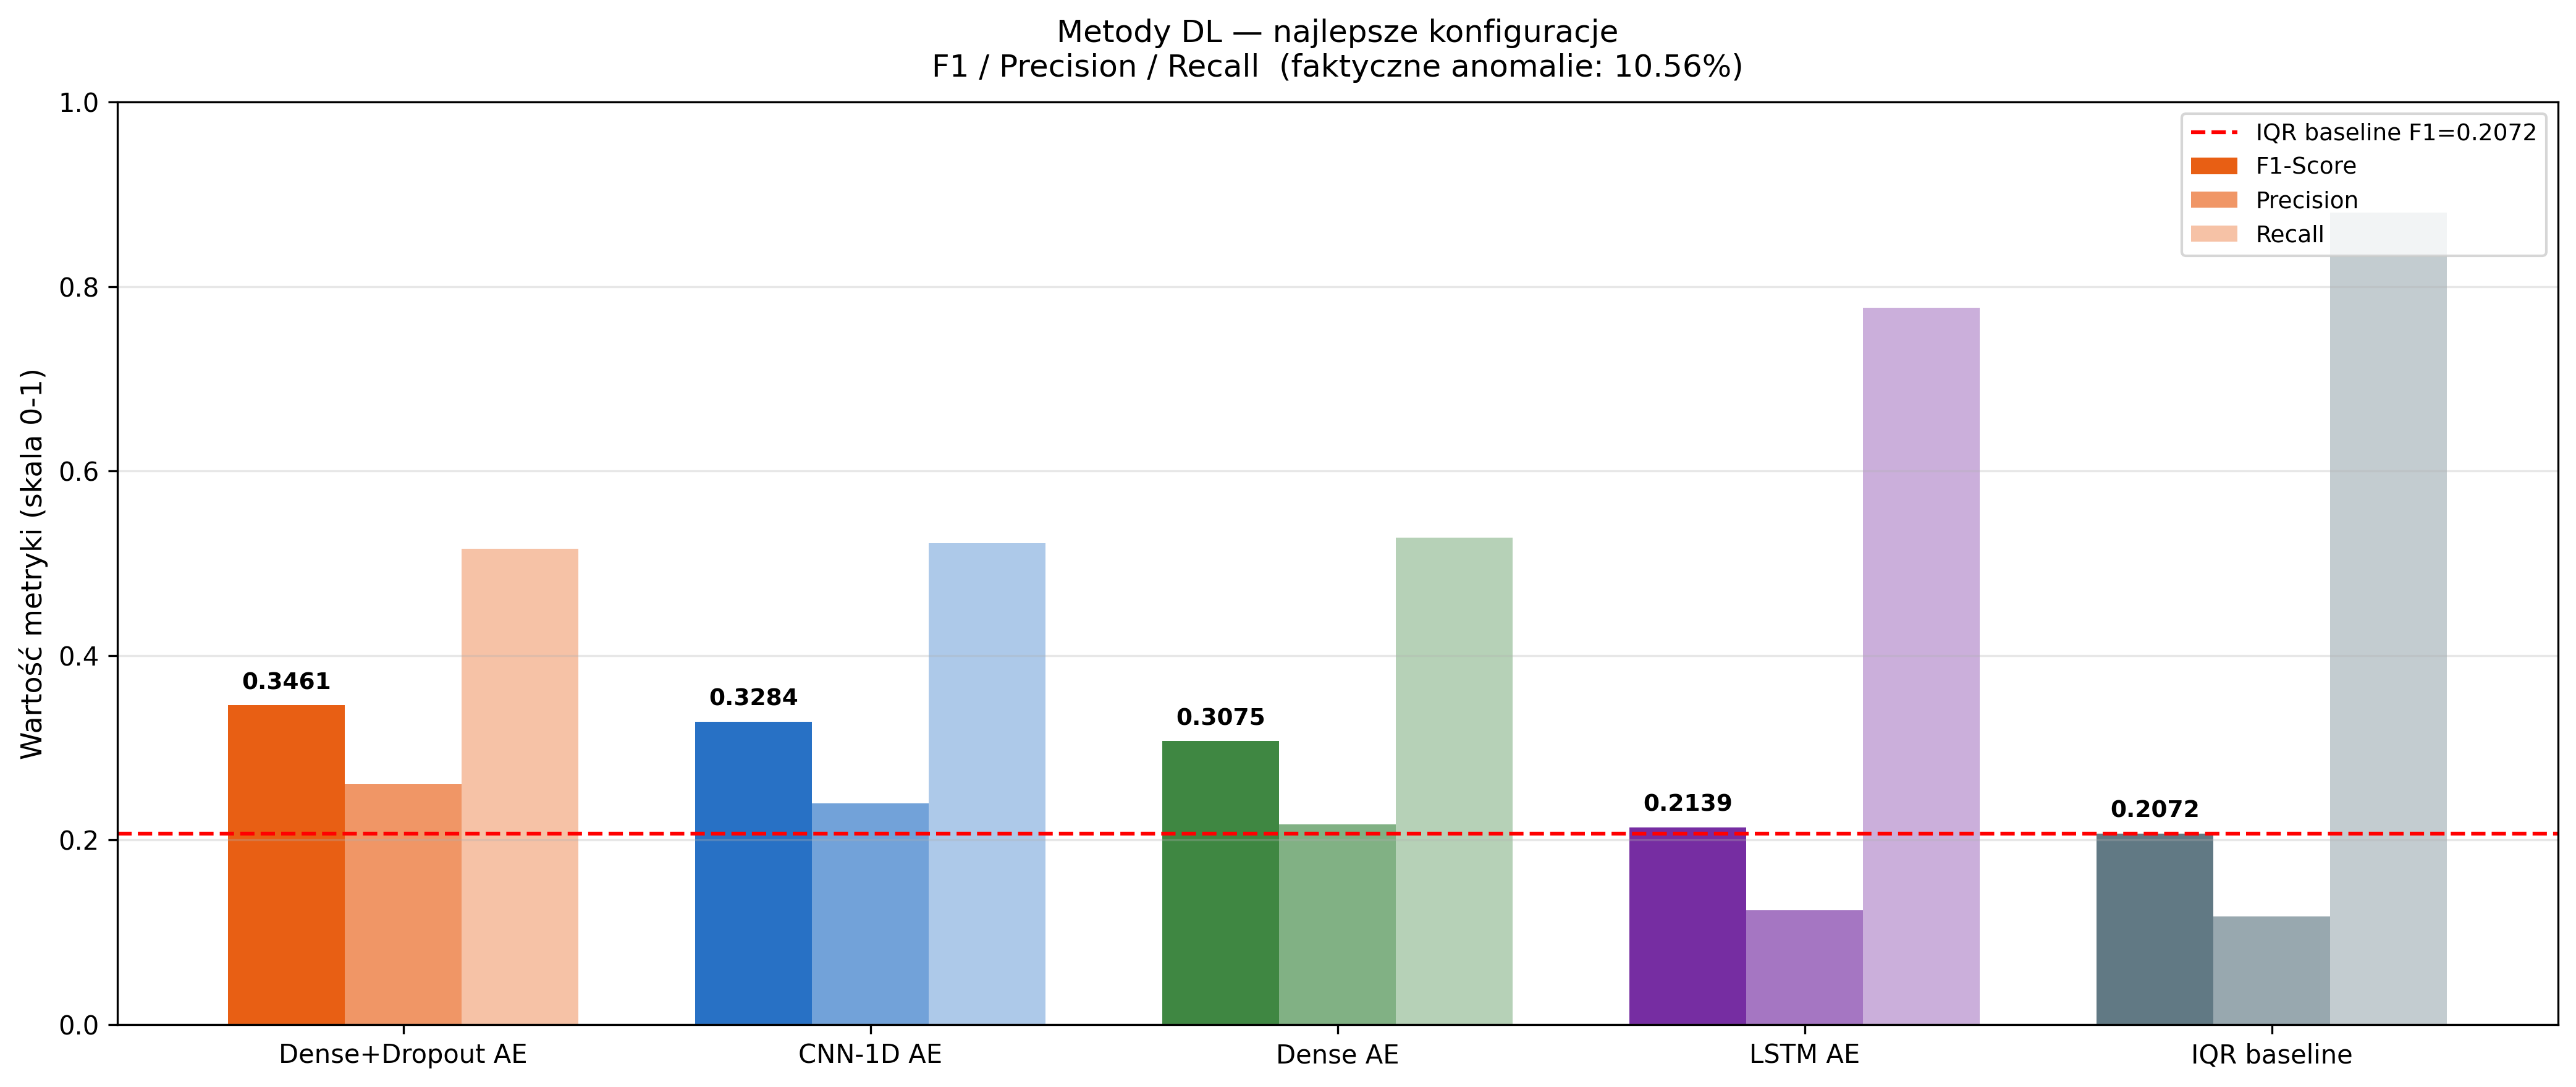
\includegraphics[width=0.9\textwidth]{fig_04b_comparison.png}
		\caption{Zestawienie skuteczności architektur opartych na głębokich sieciach neuronowych.}
		\label{fig:04b-comparison}
	\end{figure}
	
	\begin{figure}[H]
		\centering
		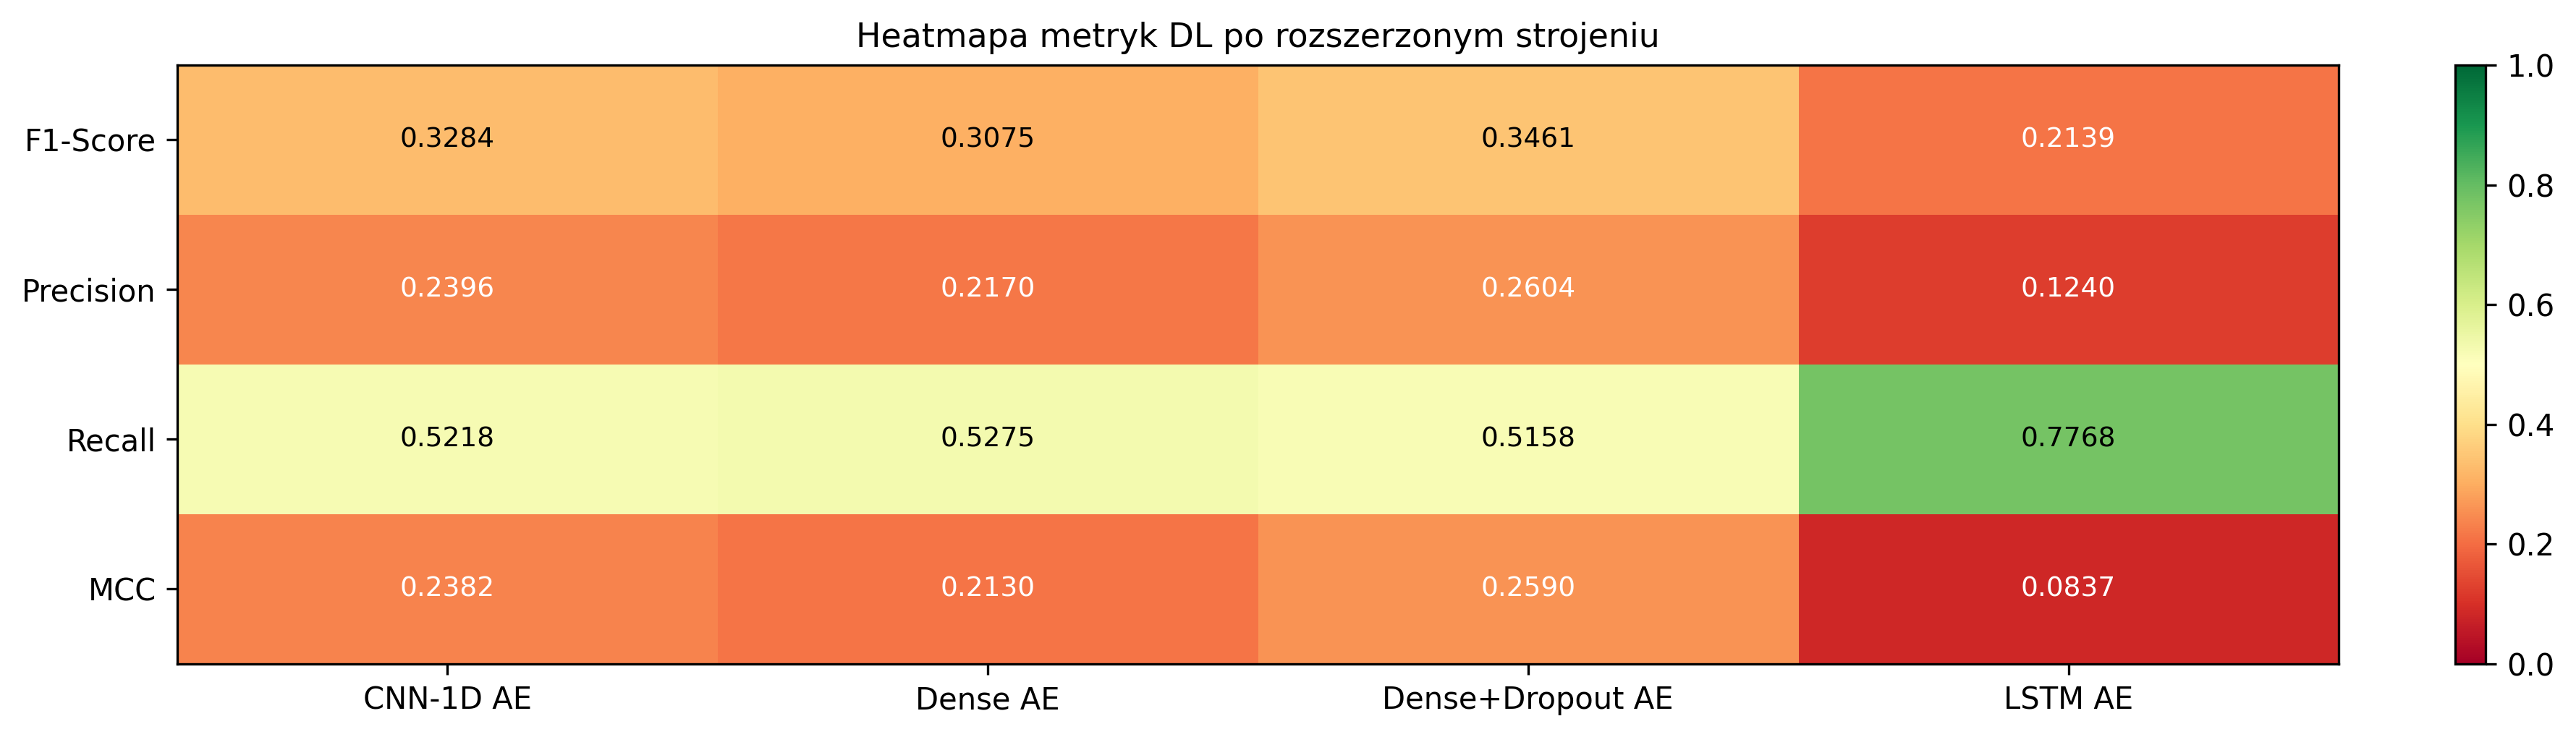
\includegraphics[width=0.9\textwidth]{fig_04b_heatmap.png}
		\caption{ Porównanie parametrów ewaluacyjnych architektur DL.}
		\label{fig:04b-heatmap}
	\end{figure}
	
	
	\section{Porównanie metod}
	\begin{table}[H]
		\centering
		\caption{Tabela porównująca wyniki wszystkich metod.}
		\label{tab:zbiorcza-wyniki}
		\begin{tabular}{lcccc}
			\toprule
			\textbf{Model} & \textbf{Typ} & \textbf{Precision} & \textbf{Recall} & \textbf{F1-Score} \\
			\midrule
			IQR & Stat. & 0.1304 & 0.7279 & 0.2211 \\
			Z-Score & Stat. & 0.1222 & 0.6446 & 0.2055 \\
			Z-Score zmodyfikowany & Stat. & 0.1311 & 0.7018 & 0.2210 \\
			CUSUM & Stat. & 0.1108 & 0.9449 & 0.1984 \\
			EWMA & Stat. & 0.1089 & 0.9999 & 0.1964 \\
			Isolation Forest & ML & 0.1823 & 0.4494 & 0.2594 \\
			Local Outlier Factor& ML & 0.2343 & 0.2874 & 0.2569 \\
			One-Class SVM & ML & 0.1280 & 0.8420 & 0.2222 \\
			K-Means & ML & ... & ... & 0.1061 \\
			Dense AE & DL & 0.2170 & 0.5275 & 0.3075 \\
			Dense+Dropout AE & DL & 0.2604 & 0.5158 & 0.3461 \\
			CNN-1D Autoenkoder & DL & 0.2396 & 0.5218 & 0.3284 \\
			LSTM AE & DL & 0.1240 & 0.7768 & 0.2139 \\
			\bottomrule
		\end{tabular}
	\end{table}
	
	\section{Koszt obliczeniowy metod}
	
	\begin{figure}
		\centering
		
\includegraphics[width=\textwidth]{fig_05_f1_vs_time.png}
		\caption{Zależność F1 od czasu wykonywania eksperymentu}
		\label{fig:05-time-memory-bubble}
	\end{figure}
	
	
	%
	% 
	%
	%Rozdział przedstawia przeprowadzone badania. Jest to zasadnicza część i~musi wyraźnie dominować w~pracy.
	%Badania i analizę wyników należy przeprowadzić, tak jak jest przyjęte w środowisku naukowym (na przykład korzystanie z danych benchmarkowych, walidacja krzyżowa, zapewnienie powtarzalności testów itd). 
	%
	%\section{Metodyka badań}
	%
	%\begin{itemize}
	%\item opis metodyki badań
	%\item opis stanowiska badawczego (opis interfejsu aplikacji badawczych -- w~załączniku)
	%\end{itemize}
	%
	%
	%\section{Zbiory danych}
	%
	%\begin{itemize}
	%\item opis danych
	%\end{itemize}
	%
	%
	%\section{Wyniki}
	%
	%\begin{itemize}
	%\item prezentacja wyników, opracowanie i poszerzona dyskusja  wyników, wnioski
	%\end{itemize}
	%
	% 
	%\begin{table}
	%\centering
	%\caption{Opis tabeli nad nią.}
	%\label{id:tab:wyniki}
	%\begin{tabular}{rrrrrrrr}
	%\toprule
	%	         &                                     \multicolumn{7}{c}{metoda}                                      \\
	%	         \cmidrule{2-8}
	%	         &         &         &        \multicolumn{3}{c}{alg. 3}        & \multicolumn{2}{c}{alg. 4, $\gamma = 2$} \\
	%	         \cmidrule(r){4-6}\cmidrule(r){7-8}
	%	$\zeta$ &     alg. 1 &   alg. 2 & $\alpha= 1.5$ & $\alpha= 2$ & $\alpha= 3$ &   $\beta = 0.1$  &   $\beta = -0.1$ \\
	%\midrule
	%	       0 &  8.3250 & 1.45305 &       7.5791 &    14.8517 &    20.0028 & 1.16396 &                       1.1365 \\
	%	       5 &  0.6111 & 2.27126 &       6.9952 &    13.8560 &    18.6064 & 1.18659 &                       1.1630 \\
	%	      10 & 11.6126 & 2.69218 &       6.2520 &    12.5202 &    16.8278 & 1.23180 &                       1.2045 \\
	%	      15 &  0.5665 & 2.95046 &       5.7753 &    11.4588 &    15.4837 & 1.25131 &                       1.2614 \\
	%	      20 & 15.8728 & 3.07225 &       5.3071 &    10.3935 &    13.8738 & 1.25307 &                       1.2217 \\
	%	      25 &  0.9791 & 3.19034 &       5.4575 &     9.9533 &    13.0721 & 1.27104 &                       1.2640 \\
	%	      30 &  2.0228 & 3.27474 &       5.7461 &     9.7164 &    12.2637 & 1.33404 &                       1.3209 \\
	%	      35 & 13.4210 & 3.36086 &       6.6735 &    10.0442 &    12.0270 & 1.35385 &                       1.3059 \\
	%	      40 & 13.2226 & 3.36420 &       7.7248 &    10.4495 &    12.0379 & 1.34919 &                       1.2768 \\
	%	      45 & 12.8445 & 3.47436 &       8.5539 &    10.8552 &    12.2773 & 1.42303 &                       1.4362 \\
	%	      50 & 12.9245 & 3.58228 &       9.2702 &    11.2183 &    12.3990 & 1.40922 &                       1.3724 \\
	%\bottomrule
	%\end{tabular}
	%\end{table}  
	%
	%
	% 
	%\begin{figure}
	%\centering
	%\begin{tikzpicture}
	%\begin{axis}[
	%    y tick label style={
		%        /pgf/number format/.cd,
		%            fixed,   % po zakomentowaniu os rzednych jest indeksowana wykladniczo
		%            fixed zerofill, % 1.0 zamiast 1
		%            precision=1,
		%        /tikz/.cd
		%    },
	%    x tick label style={
		%        /pgf/number format/.cd,
		%            fixed,
		%            fixed zerofill,
		%            precision=2,
		%        /tikz/.cd
		%    }
	%]
	%\addplot [domain=0.0:0.1] {rnd};
	%\end{axis} 
	%\end{tikzpicture}
	%\caption{Podpis rysunku po rysunkiem.}
	%\label{fig:2}
	%\end{figure}
	%
	%
	%\begin{figure}
	%\begin{lstlisting}
	%if (_nClusters < 1)
	%	throw std::string ("unknown number of clusters");
	%if (_nIterations < 1 and _epsilon < 0)
	%	throw std::string ("You should set a maximal number of iteration or minimal difference -- epsilon.");
	%if (_nIterations > 0 and _epsilon > 0)
	%	throw std::string ("Both number of iterations and minimal epsilon set -- you should set either number of iterations or minimal epsilon.");
	%\end{lstlisting}
	%\caption{Przykład pseudokodu}
	%\end{figure}
	
	
	% TODO
	
	\chapter{Podsumowanie}
	
	%\begin{itemize}
	%\item Jaki problem rozwiązałæm?
	%\item Jak ten problem rozwiązałæm?
	%\item Jakie są dobre i słabe strony mojego rozwiązania?
	%\item Czy mogę sformułować jakieś rekomendacje?
	%\end{itemize}
	
	\begin{itemize}
		\item syntetyczny opis wykonanych prac
		\item wnioski
		\item możliwość rozwoju, kontynuacji prac, potencjalne nowe kierunki
		\item Czy cel pracy zrealizowany? 
	\end{itemize}
	
	
	
	\backmatter
	
	\cleardoublepage
	\phantomsection
	%\bibliographystyle{plplain}  % bibtex
	%\bibliography{biblio} % bibtex
	\addcontentsline{toc}{chapter}{Bibliografia}
	\printbibliography           % biblatex
	
	\begin{appendices}
		
		% TODO
		\chapter{Dokumentacja techniczna}
		
		
		% TODO
		\chapter{Spis skrótów i symboli}
		
		\begin{itemize}
			\item[DNA] kwas deoksyrybonukleinowy (ang. \english{deoxyribonucleic acid})
			\item[MVC] model -- widok -- kontroler (ang. \english{model--view--controller}) 
			\item[$N$] liczebność zbioru danych
			\item[$\mu$] stopnień przyleżności do zbioru
			\item[$\mathbb{E}$] zbiór krawędzi grafu
			\item[$\mathcal{L}$] transformata Laplace'a 
		\end{itemize}
		
		% TODO
		\chapter{Lista dodatkowych plików, uzupełniających tekst pracy (jeżeli dotyczy)} 
		
		W systemie do pracy dołączono dodatkowe pliki zawierające:
		\begin{itemize}
			\item źródła programu,
			\item zbiory danych użyte w~eksperymentach,
			\item film pokazujący działanie opracowanego oprogramowania lub zaprojektowanego i wykonanego urządzenia,
			\item itp.
		\end{itemize}
		
		
		\listoffigures
		\addcontentsline{toc}{chapter}{Spis rysunków}
		\listoftables
		\addcontentsline{toc}{chapter}{Spis tabel}
		
	\end{appendices}
	
\end{document}


%% Finis coronat opus.

